\documentclass{template}
\usepackage{array}
\usepackage{graphicx}
\usepackage{float}
\usepackage{csquotes}
\usepackage[acronym, toc]{glossaries-extra}





\SetTitle{Intersektionales Wohlbefinden im Stadtraum: \\
Konzeption und Umsetzung einer App zur räumlichen Erfassung von Wohlbefinden}
\SetAuthor{Lukas Batschelet}
\SetDate{\today}

\makeglossaries

\newacronym{esm}{ESM}{Experience Sampling Method}
\newacronym{ema}{EMA}{Ecological Momentary Assessment}
\newacronym{gema}{GEMA}{Geographically Explicit Ecological Momentary Assessment}
\newacronym{drm}{DRM}{Day Reconstruction Method}
\newacronym{panas}{PANAS}{The Positive \& Negative Affect Schedule}
\newacronym{maihda}{MAIHDA}{Multilevel Analysis of Individual Heterogeneity and Discriminatory Accuracy}
\newacronym[description={Intersectional MAIHDA -- siehe \gls[noindex]{maihda}}]{i-maihda}{I-MAIHDA}{Intersectional \gls[noindex]{maihda}}
\newacronym{cart}{CART}{Classification and Regression Trees}
\newacronym{json}{JSON}{JavaScript Object Notation}
\newacronym{dsg}{DSG}{Schweizer Datenschutzgesetz}
\newacronym{dsgvo}{DSGVO}{EuropäischeDatenschutz-Grundverordnung}
\newacronym{peqi}{PEQI}{Perceived Environmental Quality Indices}
\newacronym{news}{NEWS}{Neighborhood Environment Walkability Scale}
\newacronym{health}{HEALTH}{The Healthy Environments and Active Living for Translational Health Platform}
\newacronym{mvp}{MVP}{Minimum Viable Product}
\newacronym{cicd}{CI/CD}{Continuous Integration/Continuous Delivery}
\newacronym{esec}{ESec}{European Socio-economic Classification}
\newacronym{egp}{EGP}{Erikson–Goldthorpe–Portocarero-Klassenschema}
\newacronym{wemwbs}{WEMWBS}{Warwick-Edinburgh Mental Wellbeing Scale}
\newacronym{icc}{ICC}{Intra-Class Correlation}
\newacronym{pev}{PEV}{Proportional Explained Variance}





\newacronym{vgl}{vgl.}{vergleiche}
\newacronym{bspw}{bspw.}{beispielsweise}
\newacronym{gps}{GPS}{Global Positioning System}
\newacronym{zb}{z.\,B.}{zum Beispiel}
\newacronym{ua}{u.\,a.}{unter anderem}
\newacronym{etc}{etc.}{et cetera}


\newglossaryentry{race}{
    name={\textit{race}},
    description={Eine im englischsprachigen Raum etablierte, gesellschaftlich konstruierte Kategorie, die rassifizierende Zugehörigkeiten beschreibt. In dieser Arbeit kursiv gesetzt, um ihre soziokulturelle Bedeutung zu betonen und sie deutlich vom biologistischen Begriff „Rasse“ abzugrenzen. Der Begriff verweist auf machtvolle Prozesse sozialer Differenzierung, Zugehörigkeit und Ausschluss, die historisch gewachsen sind und bis heute wirksam bleiben. Die Übertragung des Konzepts in europäische Kontexte ist umstritten: Aus Angst vor biologisierenden Implikationen und im Schatten nationaler Gewaltgeschichte (z.\,B. Nationalsozialismus) wird \textit{race} oft durch vage Begriffe wie „Ethnizität“ ersetzt oder gänzlich vermieden, was zur epistemischen Unsichtbarmachung rassifizierter Erfahrungen führen kann \parencite{bartelsPostcolonialFeminismIntersectionality2019}.},
    sort=race
}


\newglossaryentry{gender}{
    name={\textit{gender}},
    description={Bezeichnet die soziale Konstruktion von Geschlecht. Der Begriff verweist auf gesellschaftlich geprägte Vorstellungen und Erwartungen von Geschlechtsidentität. In dieser Arbeit kursiv gesetzt.},
    sort=gender
}

\newglossaryentry{schwarz}{
    name={Schwarz},
    description={Politische Selbstbezeichnung von Menschen, die im Kontext rassistischer Machtverhältnisse positioniert werden. Grossgeschrieben zur Abgrenzung von farblichen Zuschreibungen.},
    sort=schwarz
}

\newglossaryentry{intersektionalitaet}{
    name={Intersektionalität},
    description={Analytisches Konzept zur Untersuchung sich überschneidender Machtverhältnisse wie Rassismus, Sexismus, Klassismus etc. Ursprünglich von Kimberlé Crenshaw eingeführt.}
}
\newglossaryentry{class}{
    name={\textit{class}},
    description={Sozial konstruierte Kategorie, die ökonomische und symbolische Ungleichheiten beschreibt. In dieser Arbeit kursiv gesetzt.},
    sort=class
}

\newglossaryentry{reactnative}{
  name={React Native},
  description={Ein Framework zur plattformübergreifenden Entwicklung mobiler Apps. Es erlaubt die Programmierung mit \gls[noindex]{javascript} oder \gls[noindex]{typescript}, wobei der Code nativ auf Android- und iOS-Geräten ausgeführt wird. \href{https://reactnative.dev/}{reactnative.dev}}
}

\newglossaryentry{expo}{
  name={Expo},
  description={Ein Toolchain und Dienst, der die Entwicklung mit \gls[noindex]{reactnative} vereinfacht. Expo stellt Werkzeuge zum Testen, Debuggen und Veröffentlichen von Apps bereit -- ohne dass native Programmierkenntnisse erforderlich sind. \href{https://expo.dev/}{expo.dev}}
}

\newglossaryentry{supabase}{
  name={Supabase},
  description={Ein Open-Source-Backend, das als Alternative zu Firebase dient. Es basiert auf einer \gls[noindex]{datenbank} (PostgreSQL) und bietet Funktionen wie Authentifizierung, Datei-Hosting und \gls[noindex]{rls}. \href{https://supabase.com/}{supabase.com}}
}

\newglossaryentry{javascript}{
  name={JavaScript},
  description={Eine weit verbreitete Programmiersprache für Webentwicklung, die auch in mobilen Frameworks wie \gls[noindex]{reactnative} verwendet wird. Sie ist dynamisch und flexibel, aber nicht typensicher.}
}

\newglossaryentry{typescript}{
  name={TypeScript},
  description={Eine von Microsoft entwickelte Programmiersprache, die auf \gls[noindex]{javascript} basiert, aber zusätzliche statische Typisierung bietet. Sie erhöht die Wartbarkeit und Fehlervermeidung in grösseren Softwareprojekten.}
}

\newglossaryentry{python}{
  name={Python},
  description={Eine interpretierte, einfach lesbare Programmiersprache, die häufig in Wissenschaft, Datenanalyse und Automatisierung eingesetzt wird. Sie wurde auch zur Auswertung der App-Daten verwendet.}
}

\newglossaryentry{uuid}{
  name={UUID},
  description={Abkürzung für Universally Unique Identifier. Eine \textit{UUID} ist eine zufällig generierte Zeichenkette, die zur eindeutigen Identifikation eines Geräts oder Datensatzes dient, ohne personenbezogene Daten zu erfassen.},
  first={Universally Unique Identifier (\glsentrytext{uuid})}
}

\newglossaryentry{opensource}{
  name={Open-Source},
  description={Bezeichnet Software, deren Quellcode öffentlich einsehbar, veränderbar und frei verwendbar ist. \gls[noindex]{supabase} und viele Komponenten von \gls[noindex]{reactnative} und \gls[noindex]{expo} sind Open-Source.}
}

\newglossaryentry{datenbank}{
  name={Datenbank},
  description={Ein digitales System zur strukturierten Speicherung, Abfrage und Verwaltung von Daten. In der App kommt eine relationale Datenbank zum Einsatz, die durch \gls[noindex]{supabase} bereitgestellt wird.}
}

\newglossaryentry{rls}{
  name={RLS},
  description={Ein feingranulares Zugriffsmodell in einer \gls[noindex]{datenbank}, das sicherstellt, dass Nutzer:innen nur jene Datenzeilen sehen oder ändern können, für die sie berechtigt sind. \gls[noindex]{supabase} unterstützt RLS standardmässig.},
  first={Row-Level Security (\glsentrytext{rls})}
}

\newglossaryentry{github}{
  name={GitHub},
  description={Eine webbasierte Plattform zur Versionsverwaltung und Zusammenarbeit an Softwareprojekten. Sie basiert auf \gls[noindex]{git} und wird häufig zur Entwicklung und Veröffentlichung von \gls[noindex]{opensource}-Software verwendet}
}

\newglossaryentry{git}{
  name={Git},
  description={Ein verteiltes Versionskontrollsystem zur Nachverfolgung von Änderungen im Quellcode. Git ermöglicht es, Entwicklungsschritte lokal oder kollaborativ zu verwalten und ist Grundlage vieler Plattformen wie \gls[noindex]{github}}
}

\newglossaryentry{frontend}{
  name={Frontend},
  description={Der Teil einer Software, der für Nutzer:innen sichtbar und direkt bedienbar ist -- etwa die Benutzeroberfläche einer App. Wird meist in Kombination mit dem \gls[noindex]{backend} verwendet.}
}

\newglossaryentry{backend}{
  name={Backend},
  description={Der Teil einer Software, der im Hintergrund läuft und Daten verarbeitet, speichert oder bereitstellt. In dieser Arbeit wird dafür \gls[noindex]{supabase} verwendet.}
}

\newglossaryentry{framework}{
  name={Framework},
  description={Ein vorgefertigtes Gerüst für die Softwareentwicklung, das häufig genutzte Funktionen bereitstellt. \gls[noindex]{reactnative} ist ein Beispiel für ein solches Framework.},
  plural={Frameworks}
}

\newglossaryentry{pushnotification}{
  name={Push-Benachrichtigung},
  description={Eine Mitteilung, die von einer App aktiv an das Gerät gesendet wird -- auch wenn die App im Hintergrund läuft. In dieser Studie werden so die Teilnehmenden zur Beantwortung der Fragen aufgefordert.},
  plural={Push-Benachrichtigungen}
}

\newglossaryentry{ui}{
  name={UI},
  description={Die Benutzeroberfläche einer App, die für Nutzer:innen sichtbar und direkt bedienbar ist. In dieser Arbeit wird die Benutzeroberfläche der App als \gls[noindex]{ui} bezeichnet.},
  first={User Interface (\glsentrytext{ui})}
}

\newglossaryentry{postgresql}{
  name={PostgreSQL},
  description={Eine relationale \gls[noindex]{datenbank}, die als \gls[noindex]{backend} für \gls[noindex]{supabase} verwendet wird.}
}

\newglossaryentry{urbanmind}{
  name={\textit{Urban Mind}},
  description={Eine mobile App zur Echtzeit-Erhebung subjektiven Wohlbefindens mittels \gls[noindex]{gema}. Die App erfasst affektive Zustände mehrfach täglich und verknüpft sie mit räumlichen Kontexten wie Naturerleben. \glslink[noindex]{intersektionalitaet}{Intersektionale} Perspektiven werden nicht systematisch berücksichtigt. Siehe \href{https://www.urbanmind.info/}{urbanmind.info}},
  first={Urban Mind},
  sort=urbanmind
}

\newglossaryentry{reliefmaps}{
  name={\textit{Relief Maps+}},
  description={Ein webbasiertes Tool zur retrospektiven und \glslink[noindex]{intersektionalitaet}{intersektionalen} Reflexion subjektiver Raumerfahrungen. Nutzer\genderstern innen verorten emotionale Bewertungen entlang von \glspl{identitaetsachse} auf einer Karte. Siehe \href{https://reliefmaps.upf.edu/}{reliefmaps.upf.edu}},
  first={Relief Maps+},
  sort=reliefmaps
}

\newglossaryentry{intermind}{
  name={\textit{InterMind}},
  description={Eine in dieser Arbeit entwickelte \gls[noindex]{opensource}-App zur \gls[noindex]{gema}-basierten Erhebung situativer Erfahrungen. Die Entwicklung wird in \cref{sec:entwicklung_app} beschrieben. Siehe \href{https://intermind.ch/}{intermind.ch}},
  sort=intermind
}

\newglossaryentry{identitaetsachse}{
  name={Identitätsachse},
  plural={Identitätsachsen},
  description={Begriff aus der \glslink[noindex]{intersektionalitaet}{intersektionalen} Theorie, der eine einzelne soziale Kategorie wie \gls[noindex]{gender}, \gls[noindex]{race}, \gls[noindex]{class}, sexuelle Orientierung, (Dis-)Ability oder Alter bezeichnet. Solche Achsen strukturieren gesellschaftliche Positionierungen und prägen Erfahrungen von Privilegierung oder Diskriminierung.}
}

\newglossaryentry{ios}{
  name={iOS},
  description={Eine mobile Betriebssystem-Plattform, die von Apple entwickelt wird. Sie wird hauptsächlich auf Geräten des iPhone- und iPad-Produktlinien verwendet.}
}

\newglossaryentry{android}{
  name={Android},
  description={Eine mobile Betriebssystem-Plattform, die von Google entwickelt wird. Sie wird hauptsächlich auf Geräten des Android-Produktlinien verwendet.}
}

\newglossaryentry{authentifizierung}{
  name={Authentifizierung},
  description={Vorgang zur Überprüfung der Identität eines Nutzers oder Geräts, typischerweise durch die Eingabe eines Passworts, Tokens oder durch kryptografische Verfahren. In der App erfolgt die Authentifizierung gerätebasiert mittels UUID, ohne Eingabe persönlicher Informationen}
}

\newglossaryentry{autorisierung}{
  name={Autorisierung},
  description={Festlegung von Zugriffsrechten auf bestimmte Ressourcen oder Daten nach erfolgreicher Authentifizierung. In diesem Projekt bedeutet dies, dass nur das eigene Gerät auf die jeweils verknüpften Datensätze zugreifen kann (Row-Level Security)}
}

\newglossaryentry{solid}{
  name={SOLID},
  description={Akronym für fünf grundlegende Prinzipien guter objektorientierter Softwarearchitektur: \textit{Single Responsibility, Open/Closed, Liskov Substitution, Interface Segregation, Dependency Inversion}. Die Prinzipien sollen verständliche, wartbare und erweiterbare Softwaresysteme ermöglichen \parencite{martinCleanArchitectureCraftsmans2018}}
}

\newglossaryentry{emulator}{
  name={Emulator},
  plural={Emulatoren},
  description={Softwareumgebung, die ein bestimmtes Betriebssystem oder Gerät auf einem anderen System simuliert, um Programme wie auf einem echten Gerät auszuführen. In der App-Entwicklung dienen Emulatoren insbesondere dem Testen von Anwendungen auf unterschiedlichen Bildschirmgrössen, Betriebssystemversionen und Gerätearchitekturen, ohne dass reale Geräte erforderlich sind}
}

\newglossaryentry{googleplayconsole}{
  name={Google Play Console},
  description={Plattform von \gls[noindex]{google} zur Verwaltung und Verteilung von \gls[noindex]{android}-Anwendungen. Sie ermöglicht die Veröffentlichung, das Testing und das Monitoring von Apps auf Geräten mit dem Betriebssystem \gls[noindex]{android}}
}

\newglossaryentry{testflight}{
  name={TestFlight},
  description={Offizielle Plattform von Apple zur Bereitstellung von \gls[noindex]{ios}-Apps für Betatests. Entwickler\genderstern innen können damit Vorabversionen ihrer Anwendungen an registrierte Testpersonen verteilen}
}

\newglossaryentry{java}{
  name={Java},
  description={Eine streng \glslink[noindex]{objektorientierung}{objektorientierte} Programmiersprache, die in vielen Bereichen der Softwareentwicklung eingesetzt wird.}
}

\newglossaryentry{objektorientierung}{
  name={Objektorientierung},
  description={Ein Programmierparadigma, das die Entwicklung von Software durch die Modellierung von Objekten und deren Interaktionen vereinfacht. In dieser Arbeit wird die \gls[noindex]{objektorientierung} verwendet, um die App strukturiert und wartbar zu halten.}
}

\newglossaryentry{githubissue}{
    name={GitHub-Issue},
    description={Ein integriertes Werkzeug zur Aufgaben- und Projektverwaltung auf der Plattform \gls[noindex]{github}. 
    GitHub-Issues dienen der strukturierten Erfassung, Diskussion und Nachverfolgung von Aufgaben, 
    Fehlern, neuen Funktionen oder allgemeinen Projektthemen. Sie können mit Labels, Meilensteinen 
    und Verantwortlichkeiten versehen werden, um Entwicklungsprozesse transparent und nachvollziehbar zu gestalten.},
    plural={GitHub-Issues}
}

\newglossaryentry{devops}{
  name={DevOps},
  description={Ein Konzept, das die Integration von Entwicklung und Operations zusammenführt, um schnellere und stabilere Softwareentwicklung zu ermöglichen. DevOps umfasst Tools und Prozesse, die die Automatisierung von Build, Test und Bereitstellung von Software unterstützen.}
}

\newglossaryentry{meta}{
    name={Meta},
    description={US-Technologiekonzern, \gls[noindex]{ua} Entwickler von Facebook, Instagram, WhatsApp und \gls[noindex]{reactnative}.}
}

\newglossaryentry{google}{
    name={Google},
    description={US-Technologiekonzern, \gls[noindex]{ua} Betreiber von Suchmaschine, Google Play Store, YouTube und Entwickler von \gls[noindex]{firebase}.}
}

\newglossaryentry{apple}{
    name={Apple},
    description={US-Technologiekonzern, Hersteller von iPhone und Betreiber des App Store.}
}

\newglossaryentry{firebase}{
    name={Firebase},
    description={Ein \gls[noindex]{backend}-as-a-Service von \gls[noindex]{google}, das Authentifizierung, Datenspeicherung und Schnittstellenbereitstellung integriert bereitstellt.}
}

\newglossaryentry{refactoring}{
  name={Refactoring},
  description={Der Prozess der Verbesserung der Struktur und Lesbarkeit von Code, ohne dass sich die Funktionalität ändert. Refactoring ist ein wichtiger Bestandteil der Softwareentwicklung, um Code-Qualität zu erhöhen und Wartbarkeit zu verbessern.}
}

\newglossaryentry{stratum}{
    name={Stratum},
    plural={Strata},
    description={Bezeichnung für eine Teilmenge einer Grundgesamtheit in der Statistik, gebildet nach gemeinsamen Merkmalen der darin enthaltenen Beobachtungen.}
}







\AddBibFile{BA_Lukas_Batschelet.bib}


\begin{document}
\pagenumbering{gobble}

\begin{titlepage}
\sffamily
\raggedright

\vspace*{1cm}
\huge
\textbf{Intersektionales Wohlbefinden im Stadtraum}

\vspace{0.5cm}
\large
Konzeption und Umsetzung einer App zur räumlichen Erfassung von Wohlbefinden

\vspace{1.5cm}
\textbf{Lukas Batschelet}

\vspace{0.5cm}
Matrikel-Nr. 16-499-733

\vfill
\normalsize
Bachelorarbeit der Philosophisch-naturwissenschaftlichen Fakultät der Universität Bern

\vspace{0.8cm}
Betreut durch Prof. Dr. Carolin Schurr und Dr. Moritz Gubler


Geographisches Institut \\
Unit für Sozial- und Kulturgeographie\\
Bern, \today

\end{titlepage}



\newpage

\begin{abstract}
\lipsum[1]
\end{abstract}



\newpage

\pagenumbering{roman}

\tableofcontents


\newpage

% common abkürzungen beim ersten mal nicht ausführen
\glsunset{vgl}
\glsunset{bspw}
\glsunset{gps}
\glsunset{zb}

\printglossary[type=\acronymtype, title=Abkürzungsverzeichnis, toctitle=Abkürzungsverzeichnis]

\listoffigures
\listoftables


\clearpage
\pagenumbering{arabic}
% LTeX: language=de-CH
\chapter{Einleitung} \label{sec:einleitung}

Eine Parkbank am Rand eines kleinen Platzes. Beton unter den Füssen, ein Baum wirft etwas Schatten, Kinderstimmen im Hintergrund. Der Ort löst nicht bei allen dasselbe aus: Für manche bedeutet er Ruhe, für andere Anspannung oder Distanz. Solche situativen Emotionen entstehen im Zusammenspiel materieller Eigenschaften (Licht, Geräusche, Gerüche, Temperatur), sozialer Dynamiken und individueller Erfahrungen -- und sie sind durch soziale Positionierungen mitgeprägt. In dieser Arbeit rücke ich dieses situative, kontextgebundene Erleben -- \emph{affektives Wohlbefinden} -- in den Mittelpunkt.

Ich verorte die Arbeit in einer intersektionalen Perspektive, weil sie Unterschiede im Erleben nicht als Summe einzelner Merkmale versteht, sondern als Ergebnis verschränkter, machtvoll strukturierter Positionierungen. Damit rücke ich Konstellationen in den Blick, in denen Kategorien wie Geschlecht, Klasse oder Herkunft im räumlichen Kontext zusammenwirken und Erfahrungen prägen \parencite{crenshawMappingMarginsIntersectionality1991, valentineTheorizingResearchingIntersectionality2007}. In der Geographie zeigen feministische und kritisch-soziale Ansätze, wie sich solche Überschneidungen in alltäglichen Situationen materiell niederschlagen und soziale Ungleichheiten (re)produzieren \parencite{rodo-de-zarateDevelopingGeographiesIntersectionality2014, rodo-de-zarateIntersectionalityFeministGeographies2018, rodo-de-zarateIntersectionalitySpatialityEmotions2023}. Für diese Arbeit heisst das: Ich betrachte affektives Wohlbefinden als situatives, kontextgebundenes Erleben, das in der Wechselwirkung von räumlicher Materialität, sozialen Dynamiken und sozialer Positionierung entsteht -- und genau in dieser Verschränkung analysiert werden muss.

Zweitens orientiere ich mich an den \emph{affective geographies}. Sie begreifen Emotionen als verkörperte, relationale und räumlich situierte Phänomene, die zirkulieren und Zugehörigkeiten wie Distanzen herstellen \parencite{ahmedAffectiveEconomies2004}. Konzepte affektiver Atmosphären heben dabei die Spannungen von Materialität und Ideation, Bestimmtheit und Unbestimmtheit hervor und machen erfahrbar, wie Orte im Zusammenspiel von Körpern, Dingen und Sinneseindrücken wirken \parencite{andersonAffectiveAtmospheres2009}. Dieser Zugang ist für mein Vorhaben zentral, weil er den Gegenstand -- situativ-affektives Wohlbefinden -- präzise fasst, ohne ihn auf individuelle Präferenzen oder rein kognitive Bewertungen zu verkürzen, und zugleich eine explizit räumliche Analyse nahelegt \parencite{rodo-de-zarateIntersectionalitySpatialityEmotions2023}.

Drittens nehme ich eine kritisch-digitale Perspektive ein. Aus \emph{Data Feminism} folgt, dass nicht nur \emph{was} erhoben wird, sondern auch \emph{wie} und \emph{womit} eine forschungswesentliche, politische und ethische Entscheidung ist; Transparenz, Partizipation, Kontextsensibilität und Machtkritik werden damit zu Qualitätskriterien \parencite{dignazioDataFeminism2020}. Feministische Digitalgeographien zeigen zugleich, wie digitale Praktiken und Infrastrukturen ungleichheitsrelevante Einschreibungen tragen -- und warum reflektierte, situierte Datenerhebung erforderlich ist \parencite{elwoodFeministDigitalGeographies2018}. Debatten um digitale Souveränität verdeutlichen schliesslich, dass Kontrolle, Nachvollziehbarkeit und Gestaltbarkeit von Dateninfrastrukturen umkämpft sind und nicht allein technischen, sondern auch räumlich-politischen Logiken folgen \parencite{glaszeContestedSpatialitiesDigital2023}. Vor diesem Hintergrund setze ich auf eine offene, überprüfbare Infrastruktur, die Datensparsamkeit, klare Datenflüsse und Anpassbarkeit priorisiert.

Zusammengenommen bilden diese drei Perspektiven den Rahmen für mein Vorgehen. Intersektionalität lenkt den Blick auf Differenzen und Überschneidungen sozialer Positionierungen, die \emph{affective geographies} begründen, warum ich situative, räumlich gebundene Emotionen ins Zentrum rücke, und die kritisch-digitale Sicht definiert die Anforderungen an Erhebung und Verarbeitung -- Offenheit, Nachvollziehbarkeit und Datensparsamkeit. Daraus ergibt sich ein Forschungsdesign, das wiederholte, kontextnahe Erhebungen mit einer intersektionalen Auswertung auf einer offenen digitalen Grundlage verbindet. Entlang dieses Rahmens formuliere ich im Folgenden die Leitfrage sowie die drei dazugehörigen Teilfragen.



Vor diesem Hintergrund leite ich die Forschungsfragen ab. Sie rahmen die Arbeit inhaltlich, methodisch und infrastrukturell und bilden den roten Faden der folgenden Kapitel.

\begin{quote}
\emph{Wie lässt sich der Einfluss räumlicher Umgebungen auf das affektive Wohlbefinden intersektional positionierter Personen erfassen und analysieren?}
\end{quote}

\begin{enumerate}
    \item Welche Merkmale muss ein Erhebungsansatz aufweisen, um affektives Wohlbefinden intersektional positionierter Personen gemeinsam mit relevanten Kontextmerkmalen wiederholt in situ zu erfassen?
    \item Welche Anforderungen ergeben sich aus einer kritisch-digitalen Perspektive an ein Werkzeug, das solche Erhebungen ermöglicht, und wie realisiere ich diese Anforderungen in einer konkreten Umsetzung?
    \item Wie geeignet sind die in einer Pilotstudie erhobenen Daten für eine intersektionale Mehrebenenmodellierung?
\end{enumerate}

Methodisch verorte ich die Arbeit im Feld wiederholter, kontextgebundener Befragungen: Ich diskutiere, wie \gls[noindex]{ema}/\gls[noindex]{gema} die unmittelbare Erfassung situativer Emotionen ermöglichen und wie sich diese Logik mit intersektionalen Auswertungsansätzen verbinden lässt. Analytisch prüfe ich, ob die in der Pilotierung gewonnenen Daten die Grundvoraussetzungen einer intersektionalen Mehrebenenanalyse erfüllen.

Infrastrukturell entwickle ich mit \gls[noindex]{intermind}\footnote{\href{https://intermind.ch/app}{intermind.ch/app}} eine offene \gls[noindex]{gema}-Infrastruktur. Die App befragt Teilnehmende über einen festgelegten Zeitraum hinweg wiederholt und erfasst Antworten zusammen mit standortbezogenen Kontextinformationen in Echtzeit; alle Daten werden anonymisiert gespeichert. Die quelloffene Auslegung ermöglicht Anpassungen an andere Forschungskontexte und schafft eine Grundlage für eine transparente, langfristig nutzbare Infrastruktur zur Erhebung kontextualisierter Alltagsdaten.

Aus den Forschungsfragen leite ich die Anforderungen an den Fragebogen ab und entwickle darauf aufbauend eine kompakte Erhebung. Der Fragebogen bildet das thematische Feld präzise ab, hält die Teilnahmebelastung gering und schafft die Voraussetzung für eine intersektionale Auswertung.

In einer explorativen Pilotstudie erprobe ich das Zusammenspiel aus Infrastruktur, Erhebungsdesign und Auswertungspfad. Dabei prüfe ich, ob die erhobenen Daten die erforderliche Differenzierung und Qualität für eine intersektionale Mehrebenenanalyse aufweisen und wo die Grenzen des Ansatzes liegen. Die Pilotierung dient dem methodischen Machbarkeitsnachweis; inhaltliche Effektschätzungen und Generalisierungen sind nicht Ziel dieser Arbeit.

Um die Forschungsfragen zu beantworten, führe ich die Lesenden zunächst in \Cref{sec:theoretischer_rahmen} in zentrale Begriffe und Konzepte ein -- darunter (i) Intersektionalität als Analyseinstrument, (ii) affektives Wohlbefinden als räumlich situierte Erfahrung und (iii) kritisch-digitale Perspektiven auf Forschungsinfrastrukturen. Darauf aufbauend erläutere ich in \Cref{sec:methodik} das methodische Vorgehen: von den theoretischen Grundlagen wiederholter Befragung über konzeptionelle Entscheidungen bis hin zur Einordnung des gewählten Zugangs im Vergleich zu bestehenden Instrumenten. Die Entwicklung der App \gls[noindex]{intermind} und die zugrunde liegenden Anforderungen thematisiere ich in \Cref{sec:entwicklung_app}, bevor ich in \Cref{sec:fragebogenentwicklung} die Konstruktion des Fragebogens darstelle. Anschliessend widme ich mich in \Cref{sec:pilotstudie} der Durchführung und Analyse der explorativen Pilotstudie. Den Abschluss bildet \Cref{sec:diskussion}, in dem ich zentrale Befunde reflektiere, methodische Implikationen diskutiere und Perspektiven für künftige Forschung skizziere.

Mit dieser Arbeit leiste ich einen explorativen Beitrag, der methodische Innovationen mit gesellschaftlich relevanten Fragestellungen verbindet. Ich erhebe keinen Anspruch auf allgemeine Repräsentativität; im Zentrum steht, methodische Potenziale und erste Ansätze für zukünftige intersektionale Analysen des situativen Wohlbefindens in alltäglichen Umgebungen aufzuzeigen.




\newpage

% LTeX: language=de-CH

\section{Theoretischer Rahmen} \label{sec:theoretischer_rahmen}

\subsection{Intersektionalität in der quantitativen Forschung}

\subsubsection{Definition und Ursprünge der Intersektionalität}

Der Begriff der \gls{intersektionalitaet} wurde ursprünglich von Kimberlé \textcite{crenshawMappingMarginsIntersectionality1991} geprägt und verweist auf die Überlagerung und wechselseitige Verstärkung unterschiedlicher Formen von Diskriminierung, insbesondere im Kontext von \gls{race} und \gls{gender}\footnote{\gls{race} und \gls{gender} werden in dieser Arbeit kursiv gesetzt, um auf ihre Bedeutung als gesellschaftlich konstruierte, aber wirkmächtige Kategorien hinzuweisen. \textit{race} verweist auf rassifizierende Zugehörigkeitszuschreibungen, die historisch gewachsen sind und soziale Ungleichheiten produzieren. \gls{gender} beschreibt die soziale Konstruktion von Geschlecht und verweist auf normative Vorstellungen von Weiblichkeit, Männlichkeit oder anderen Geschlechtsidentitäten. Die Begriffe werden im englischen Original verwendet, da adäquate deutsche Entsprechungen fehlen oder missverständlich sind \parencite[vgl.][]{hallRaceArticulationSocieties1980, butlerGenderTroubleFeminism1990}} \parencite{hancockWhenMultiplicationDoesnt2007}.
Ausgangspunkt dieser theoretischen Perspektive ist die Black Feminist Theory, welche unter anderen in den Arbeiten von Crenshaw sowie Patricia Hill \textcite{collinsBlackFeministThought2002}, Audre Lorde und Bell Hooks ihren Ausdruck findet. Black Feminist Theory formulierte eine scharfe Kritik an traditionellen feministischen Ansätzen, denen vorgeworfen wurde, primär die Erfahrungen weisser, privilegierter Frauen ins Zentrum zu stellen und somit die Lebensrealitäten Schwarzer\footnote{„\gls{schwarz}“ wird in dieser Arbeit als politische Selbstbezeichnung Schwarzer Menschen mit grossem Anfangsbuchstaben verwendet. Der Begriff beschreibt keine biologische Eigenschaft, sondern eine soziale Positionierung im Kontext rassistischer Machtverhältnisse. Die Grossschreibung dient der Abgrenzung von farblichen oder äusserlichen Zuschreibungen \parencite[vgl.][]{oguntoyeFarbeBekennenAfrodeutsche1986}.} Frauen zu marginalisieren \parencite{collinsBlackFeministThought2002}. Crenshaw entwickelte das Konzept der Intersektionalität explizit als Reaktion auf die Unfähigkeit bestehender theoretischer Ansätze, die spezifischen Diskriminierungserfahrungen Schwarzer Frauen adäquat zu erfassen. Dabei verdeutlichte sie, dass Diskriminierung nicht als Summe einzelner, isolierter Erfahrungen verstanden werden könne, sondern als eigenständige Form sozialer Benachteiligung, die sich an der Überschneidung sozialer Kategorien wie \gls{race}, \gls{gender} und \gls{class} manifestiert \parencite{crenshawMappingMarginsIntersectionality1991}.

Intersektionalität entwickelte sich somit nicht allein im akademischen Kontext, sondern ist stark verwurzelt in den politischen Kämpfen sozialer Bewegungen, insbesondere im Kontext feministischer, antirassistischer und antikapitalistischer Aktivismen der 1970er- und 1980er-Jahre \parencite{collinsBlackFeministThought2002}. Zentral für die theoretische Grundlage des intersektionalen Ansatzes ist die Anerkennung von Machtverhältnissen und sozialen Ungleichheiten als strukturell verankert und historisch bedingt. Gesellschaftliche Positionierungen wie \textit{gender}, \textit{race} oder \textit{class} werden hierbei als sozial konstruierte Kategorien verstanden, die immer in Verbindung mit bestehenden Machtsystemen wie Sexismus, Rassismus oder Klassismus betrachtet werden müssen. Audre Lorde und Bell Hooks betonten insbesondere die Rolle struktureller Unterdrückung und verdeutlichten, wie sich dominante Gesellschaftsstrukturen auf individueller Ebene reproduzieren und sich somit wechselseitig verstärken \parencite{collinsBlackFeministThought2002, hancockWhenMultiplicationDoesnt2007}.

Von der ursprünglich starken Fokussierung auf \textit{race} und \textit{gender} wurde das Konzept der Intersektionalität in den folgenden Jahrzehnten zunehmend erweitert und schliesst heute eine Vielzahl sozialer Positionierungen und Identitäten ein, darunter etwa Sexualität, Alter, Behinderung, Nationalität oder Religion \parencite{bauerIntersectionalityQuantitativeResearch2021, bowlegInvitedReflectionQuantifying2016}. Diese Erweiterung verdeutlicht die breite theoretische und empirische Anwendbarkeit von Intersektionalität als Analyseinstrument zur kritischen Untersuchung gesellschaftlicher Ungleichheiten und Diskriminierungserfahrungen. Intersektionalität hat sich somit nicht nur als theoretisches Konzept, sondern auch als methodische Grundlage etabliert, welche insbesondere in feministischen, sozialwissenschaftlichen und zunehmend auch in quantitativ orientierten Diskursen verwendet wird, um die komplexen Wechselwirkungen gesellschaftlicher Machtverhältnisse zu analysieren.


\subsubsection{Quantitative Ansätze und ihre Herausforderungen}

Quantitative Forschungsmethoden gewinnen in der intersektionalen Forschung zunehmend an Bedeutung, wobei unterschiedliche theoretische und methodische Ansätze verfolgt werden \parencite{bauerIntersectionalityQuantitativeResearch2021}. Quantitative Verfahren bieten das Potenzial, systematische Strukturen und Muster von Interaktionen zwischen sozialen Kategorien empirisch sichtbar und statistisch überprüfbar zu machen. Gleichzeitig ist jedoch die methodische Umsetzung intersektionaler Analysen mit erheblichen Herausforderungen verbunden.

Ein grundlegendes Spannungsfeld ergibt sich aus der Integration der theoretischen Prämissen der Intersektionalität mit den technischen Anforderungen quantitativer Analysen. So kritisieren \textcite{hancockWhenMultiplicationDoesnt2007} eindimensionale und additive statistische Modelle, welche soziale Kategorien als unabhängige Variablen betrachten und lediglich deren einzelne Haupteffekte untersuchen. Solche Modelle laufen Gefahr, die Kernannahme der Intersektionalität, wonach soziale Kategorien stets miteinander verschränkt sind, unzureichend abzubilden \parencite{bowlegInvitedReflectionQuantifying2016, bauerIntersectionalityQuantitativeResearch2021}. In der Praxis wird Intersektionalität häufig auf einfache Interaktionseffekte in Regressionsmodellen reduziert, was die Gefahr einer Fehlinterpretation oder Vereinfachung komplexer sozialer Realitäten birgt \parencite{bauerIntersectionalityQuantitativeResearch2021, scottIntersectionalityQuantitativeMethods2017}.

Besonders zentral ist in diesem Zusammenhang die Frage nach der kontextsensitiven Operationalisierung intersektionaler Kategorien. Eine blosse Festlegung statischer sozialer Gruppen reicht nicht aus, da soziale Kategorien wie \textit{race} oder \textit{gender} stets kontextabhängig und multidimensional konstruiert sind. Maria \textcite{rodo-de-zarateDevelopingGeographiesIntersectionality2014} argumentiert, dass quantitative Verfahren entsprechend flexibilisiert und angepasst werden müssen, um der Dynamik und Fluidität sozialer Identitäten gerecht zu werden. Dies erfordert eine hohe theoretische Reflexivität und methodologische Sensibilität, insbesondere bezüglich der Validität verwendeter Messinstrumente sowie der Interpretation statistischer Ergebnisse \parencite{bauerIntersectionalityQuantitativeResearch2021, websterCenteringSocialtechnicalRelations2021}.

Um diesen Herausforderungen zu begegnen, wurden unterschiedliche methodische Ansätze entwickelt. Ein vielversprechender Ansatz ist die \acrfull{maihda}, welche es erlaubt, intersektionale Effekte differenziert abzubilden, indem sie systematisch Varianzen innerhalb und zwischen sozialen Positionen quantifiziert \parencite{evansTutorialConductingIntersectional2024, grossModellingIntersectionalityQuantitative2023, axelssonfiskChronicObstructivePulmonary2018}. \gls{maihda} bietet insbesondere die Möglichkeit, eine grosse Anzahl sozialer Positionierungen gleichzeitig zu betrachten, ohne diese auf blosse Interaktionsterme in klassischen Regressionsmodellen zu reduzieren \parencite{bauerIntersectionalityQuantitativeResearch2021}.

Ein Beispiel für die praktische Anwendung von \gls{maihda} liefert die Studie von \textcite{axelssonfiskChronicObstructivePulmonary2018}, in der die Verteilung von Lungenerkrankungen (COPD) unter mehr als 2{,}4 Millionen Menschen in Schweden untersucht wurde. Die Forschenden kombinierten dabei soziale Merkmale wie Alter, Geschlecht, Einkommen, Bildung, Familienstand und Migrationsstatus zu 96 verschiedenen sozialen Gruppen (sogenannten intersektionalen Strata). Durch die MAIHDA-Analyse konnte sichtbar gemacht werden, welche dieser Gruppen besonders stark oder schwach von der Erkrankung betroffen waren. Besonders auffällig war etwa, dass alleinlebende ältere Frauen mit niedrigem Einkommen und geringer Bildung ein bis zu 49-mal höheres Erkrankungsrisiko hatten als junge Männer mit hoher Bildung, gutem Einkommen und stabiler Partnerschaft. Die Studie zeigt exemplarisch, wie mit MAIHDA komplexe soziale Ungleichheiten im Gesundheitsbereich nicht nur statistisch erfasst, sondern auch differenziert beschrieben werden können. Gleichzeitig zeigte sich, dass viele dieser Unterschiede nicht durch besondere Wechselwirkungen (Interaktionen), sondern vor allem durch die Summe sozialer Nachteile erklärbar sind. 

Eine weitere Perspektive eröffnen sogenannte \emph{Decision-Tree}-Verfahren wie Klassifikations- und Regressionsbäume (\acrshort{cart}), welche explorativ heterogene Muster innerhalb intersektionaler Gruppen offenlegen können. Diese Verfahren sind insbesondere geeignet, wenn lineare Modellannahmen nicht greifen oder wenn vermutet wird, dass Schwellenwerte oder spezifische Kombinationen sozialer Merkmale entscheidend sind. CART-Verfahren sind jedoch durch ihre Datenabhängigkeit, begrenzte Generalisierbarkeit und eingeschränkte Reproduzierbarkeit limitiert \parencite{bauerIntersectionalityQuantitativeResearch2021}.

Ein zentraler methodologischer Diskussionspunkt betrifft zudem die Frage, wie intersektionale Kategorien in quantitativen Analysen konzeptualisiert werden. Leslie \textcite{mccallComplexityIntersectionality2005} entwickelte hierfür eine dreiteilige Typologie, die zwischen einer zwischenkategorialen (\textit{intercategorical}) und einer innerkategorialen (\textit{intracategorical}) Herangehensweise unterscheidet. Während zwischenkategoriale Analysen Unterschiede zwischen verschiedenen sozialen Gruppen systematisch vergleichen, richten sich innerkategoriale Ansätze auf die Untersuchung von Heterogenität und Dynamiken innerhalb einer bestimmten Gruppe oder sozialen Positionierung \parencite{bauerAdvancingQuantitativeIntersectionality2019}. Die Wahl der jeweiligen Herangehensweise beeinflusst massgeblich die Operationalisierung intersektionaler Kategorien sowie die Auswahl und Interpretation quantitativer Verfahren.

Trotz der genannten Herausforderungen bieten quantitative Verfahren jedoch bedeutende Chancen für die intersektionale Forschung. Sie ermöglichen es, sozialstrukturelle Ungleichheiten empirisch sichtbar zu machen, grössere Stichproben systematisch zu untersuchen und somit evidenzbasierte Handlungsempfehlungen abzuleiten. Um quantitative Methoden adäquat für intersektionale Analysen nutzen zu können, ist es jedoch zwingend erforderlich, methodische Innovationen aktiv weiterzuentwickeln sowie eine kritische und reflektierte Anwendung der verfügbaren statistischen Verfahren sicherzustellen \parencite{bauerIntersectionalityQuantitativeResearch2021, bauerAdvancingQuantitativeIntersectionality2019, scottIntersectionalityQuantitativeMethods2017}.


\subsection{Räumliche Umgebung und affektives Wohlbefinden}

\subsubsection{Affektives Wohlbefinden}

Mit dem sogenannten \emph{emotional turn} hat sich die Geographie seit den frühen 2000er‑Jahren intensiv der Frage gewidmet, wie Emotionen und Affekte in und durch Räume entstehen \parencite{hoSocialGeographyIII2024}. Im Zentrum steht dabei das Konzept des affektiven Wohlbefindens: Es bezeichnet kurzfristige, situativ schwankende Gefühlslagen wie Freude, Gelassenheit oder Anspannung, die besonders sensibel auf Kontexteinflüsse reagieren. 

Die zentrale Einsicht dieses Paradigmenwechsels besteht darin, dass solche Gefühle nicht ausschliesslich im Inneren von Individuen entstehen, sondern durch ihr Zirkulieren zwischen Körpern, Dingen und Orten soziale Wirklichkeit mitgestalten. Sara \textcite{ahmedAffectiveEconomies2004} beschreibt diese Dynamik als \emph{affective economies}: Gefühle „haften“ an Gegenständen, Räumen oder Personengruppen und erzeugen dadurch Grenzziehungen zwischen Eigenem und Fremdem. Anderson greift diesen Gedanken auf und spricht von atmosphärischen Stimmungsschichten, die Orte wie ein kaum sichtbarer Schleier durchziehen und das Erleben aller Anwesenden prägen \parencite{andersonAffectiveAtmospheres2009}. Elaine \textcite{hoSocialGeographyIII2024} fasst die aktuelle Forschung zu diesen affektiven Raumqualitäten zusammen und betont, dass sich Gefühle stets in bestehende Macht‑ und Ungleichheitsverhältnisse einschreiben.

Für diese Arbeit bedeutet das: Affektives Wohlbefinden entsteht nicht im luftleeren Raum, sondern im Zusammenspiel von materieller Ausstattung (etwa Vegetation oder Lärmpegel), sozialer Situation und den historisch gewachsenen Bedeutungen, die einem Ort anhaften.


\subsubsection{Methodische Zugänge und empirische Befunde}

Erste Versuche, affektives Wohlbefinden empirisch zu erfassen, stützten sich auf klassische Befragungen oder Laborexperimente – Methoden, die die situative Eingebundenheit emotionaler Zustände jedoch nur unzureichend abbilden konnten \parencite{kirchnerSpatiotemporalDeterminantsMental2016}. Einen grundlegenden methodischen Fortschritt brachte die Entwicklung der \acrfull{esm}, bei der Teilnehmende mehrmals täglich per Smartphone kurze Angaben zu ihrer momentanen Stimmung, Tätigkeit und sozialen Situation machen. Aufbauend darauf verbindet die \acrfull{gema} diese subjektiven Angaben mit GPS‑Daten sowie externen Umweltdaten – etwa Vegetationsanteil, Verkehrsaufkommen oder Wetter – und erlaubt so eine präzise räumlich‑zeitliche Analyse affektiver Erfahrungen \parencite{kirchnerSpatiotemporalDeterminantsMental2016}.

Auf Grundlage dieser Instrumente zeigen sich in der Literatur drei wiederkehrende Befundlinien:

Erstens deuten zahlreiche Studien auf eine positive Wirkung naturräumlicher Qualitäten hin. \textcite{birenboimInfluenceUrbanEnvironments2018} analysierten über 5'000 \gls{esm}-Einträge aus verschiedenen urbanen Kontexten und zeigten, dass Parkanlagen, baumgesäumte Strassen und visuell offene Plätze das Sicherheits- und Komfortempfinden erhöhen, während stark befahrene Verkehrsachsen gegenteilige Effekte zeigen. Eine \gls{gema}-Studie von \textcite{mascherekMeadowsAsphaltRoad2025} ergänzt, dass Sonnenschein, das Unterwegssein mit Freund:innen und aktive Mobilität stärkere Effekte auf affektives Wohlbefinden haben als die blosse Präsenz von Grünflächen. \textcite{hammoudSmartphonebasedEcologicalMomentary2024} heben insbesondere die Rolle ökologischer Vielfalt hervor: Je abwechslungsreicher die natürliche Ausstattung eines Orts (etwa durch Bäume, Pflanzen oder Vogelgesang), desto höher die berichteten Werte des Wohlbefindens. Auch unter pandemiebedingten Einschränkungen blieben solche Effekte bestehen: Während der COVID‑19‑Lockdowns gewannen Aufenthalte in Grün- und Blauräumen für viele Menschen therapeutische Bedeutung \parencite{doughtyTherapeuticLandscapesCOVID192023}.

Zweitens zeigen sich klare Differenzen darin, wie Menschen Räume affektiv erleben – je nach sozialer Positionierung. So beschreibt \textcite{shakerSayingNothingSaying2021}, wie alltägliche Fahrten mit dem öffentlichen Verkehr für junge Muslim\genderstern innen in Amsterdam durch subtile Blicke oder Gesten zu Räumen latenter Bedrohung werden können. \textcite{hallHatescapeRelationalGeography2019} dokumentieren ähnliche Erfahrungen bei Menschen mit Behinderung, für die bestimmte urbane Räume durch wiederholte Mikroaggressionen zu sogenannten Hatescapes werden. Diese empirischen Arbeiten unterstreichen die Notwendigkeit, Macht- und Ungleichheitsverhältnisse systematisch in die Analyse affektiver Raumwahrnehmung einzubeziehen \parencite{hoSocialGeographyIII2024}.

Drittens wird in der Literatur zunehmend zwischen kurzfristigem affektivem Erleben und langfristiger Lebenszufriedenheit unterschieden. \textcite{chenPerceivedUrbanEnvironment2025} zeigen, dass ruhige, naturnahe Orte vor allem das unmittelbare emotionale Erleben verbessern, während kulturelle Angebote, Bildungseinrichtungen oder gastronomische Infrastruktur eher mit langfristiger Zufriedenheit assoziiert sind. Lärmintensive und hochverdichtete städtische Räume stehen hingegen konsistent im negativen Zusammenhang mit affektivem Wohlbefinden.

Insgesamt belegt die empirische Forschung, dass affektives Wohlbefinden ein sensibles Produkt aus räumlichen, sozialen und situativen Faktoren ist. Dank \gls{esm} und \gls{gema} lassen sich diese komplexen Zusammenhänge inzwischen so erfassen, dass Stadtplanung und Public Health gezielt auf sie reagieren können – etwa durch die Förderung biodiversitätsreicher Grünflächen, sozial nutzbarer Rückzugsorte oder durch Massnahmen zur Lärmminderung an belasteten Verkehrsräumen \parencite{cookeMeasuringWellBeingReview2016}.

\subsection{Bedeutung intersektionaler Perspektiven auf affektives Wohlbefinden}

Die empirische Literatur zeigt überzeugend, dass räumliche Kontexte das affektive Wohlbefinden prägen. Weniger gut verstanden ist jedoch, wie sich diese situativen Gefühlslagen mit sozialen Machtachsen – etwa \textit{gender}, \textit{race} und \textit{class} – verschränken. Genau hier setzt die intersektionale Geographie an: Sie verknüpft emotionale Raumforschung mit der Analyse mehrfacher Ungleichheiten und fragt, wie Orte für verschiedene Körper zugleich befreiend oder belastend sein können \parencite{rodo-de-zarateIntersectionalityFeministGeographies2018}. 

Rodó‑de‑Zárate entwickelt dafür das Instrument der \textit{Relief Maps}, das soziale Positionierungen, geographische Orte und subjektives (Un‑)Behagen in einer Matrix zusammenführt \parencite{rodo-de-zarateDevelopingGeographiesIntersectionality2014}. Ihre Studien mit jungen lesbischen Frauen zeigen, dass Sicherheitsempfinden im öffentlichen Raum nicht im Ort selbst liegt, sondern in der relationalen Überlagerung räumlicher Strukturen mit sozialen Kategorien \textcite{rodo-de-zarateYoungLesbiansNegotiating2015}. In einer jüngeren Arbeit betont sie, dass Emotionen—verstanden als (Dis)comforts—räumliche Indikatoren für intersectionale Machtgeometrien sind: Wer welchen Platz „bewohnen“ kann, entscheidet sich an der Schnittstelle von Gefühl und Raum \parencite{rodo-de-zarateIntersectionalitySpatialityEmotions2023}. 

Diese Befunde machen deutlich, dass affektives Wohlbefinden räumlich ungleich verteilt ist. Es entsteht in situativen Atmosphären, die für marginalisierte Gruppen von Mikroaggressionen, Blicken oder architektonischen Barrieren durchzogen sein können \parencite{websterCenteringSocialtechnicalRelations2021}. Eine intersektionale Perspektive legt somit offen, warum dieselbe Grünfläche für eine Person Ruhe stiftet, für eine andere aber Stress auslöst. Sie erweitert die Forschung zu affektiven Atmosphären um eine machtanalytische Dimension und liefert praxisnahe Hinweise für eine Stadtplanung, die soziale Gerechtigkeit und emotionale Zugänglichkeit gleichermassen berücksichtigt.




\clearpage

% LTeX: language=de-CH

\section{Methodisches Vorgehen} \label{sec:methodik}

\subsection{Methodischer Ansatz der Studie}

\subsubsection{Echtzeiterhebungen mittels wiederholter Befragung (Experience Sampling)}

Die Erhebung von momentanen Wohlbefindenszuständen setzt methodisch voraus, dass subjektive Erfahrungen möglichst zeitnah und kontextsensitiv gemessen werden. Retrospektive Selbstberichte sind typischerweise anfällig für Verzerrungen, die durch selektive Erinnerung oder nachträgliche Neubewertungen entstehen (\textit{Recall Bias}), und daher nur begrenzt geeignet, um flüchtige affektive Zustände präzise abzubilden \parencite{kahnemanDevelopmentsMeasurementSubjective2006}. Als methodische Antwort auf diese Herausforderung etablierte sich das sogenannte Experience Sampling, auch als Ecological Momentary Assessment (\acrshort{ema}) bekannt. Dieser Ansatz basiert auf wiederholten, situativ eingebetteten Messungen, welche affektive, kognitive oder auch verhaltensbezogene Zustände unmittelbar während oder kurz nach dem Erleben erfassen \parencite{birenboimInfluenceUrbanEnvironments2018, kirchnerSpatiotemporalDeterminantsMental2016}.

In der vorliegenden Studie wird dieser methodische Zugang genutzt, um individuelle Wohlbefindenszustände und deren räumlichen Kontext systematisch zu erfassen. Durch den Einsatz einer eigens entwickelten Smartphone-Applikation erfolgt die Datenerhebung in Echtzeit und räumlich exakt, da neben der unmittelbaren affektiven Selbsteinschätzung auch Geolokationsdaten automatisiert gespeichert werden. Die Verwendung einer Smartphone-basierten Methodik erlaubt somit eine exakte Zuordnung von affektiven Zuständen zu spezifischen räumlichen Umgebungen. Damit folgt der methodische Ansatz aktuellen Empfehlungen der Forschung, wonach insbesondere die Kombination von Experience Sampling mit ortsbezogenen Daten (Geographically Explicit Ecological Momentary Assessment; \acrshort{gema}) eine differenzierte Analyse situativer und räumlicher Einflüsse auf das Wohlbefinden ermöglicht \parencite{mascherekMeadowsAsphaltRoad2025, kirchnerSpatiotemporalDeterminantsMental2016}.

Die Entscheidung für wiederholte Messungen innerhalb einer Person bietet gegenüber Querschnittstudien deutliche methodische Vorteile. Erstens erhöht die wiederholte intraindividuelle Datenerhebung die Präzision der Messungen und reduziert Verzerrungen, da interpersonelle Differenzen in der affektiven Bewertung von Situationen kontrolliert werden können. Zweitens erlaubt sie, kurzfristige Schwankungen und Dynamiken im Wohlbefinden abzubilden, die für langfristige Lebenszufriedenheitsskalen unerreichbar bleiben. Drittens bietet ein solches Studiendesign die Möglichkeit, situative Kontexteffekte unmittelbar zu analysieren und damit detailliert zu identifizieren, welche räumlichen Faktoren Wohlbefinden positiv oder negativ beeinflussen \parencite{birenboimInfluenceUrbanEnvironments2018, hammoudSmartphonebasedEcologicalMomentary2024}.

Zur Erfassung des momentanen Wohlbefindens wurden numerische Skalen eingesetzt, welche sowohl die Belastung der Teilnehmenden reduzieren als auch valide und vergleichbare Daten generieren \parencite{cookeMeasuringWellBeingReview2016}. Gleichzeitig erfolgte die automatische Erfassung räumlicher Kontexte mithilfe integrierter GPS-Funktionalitäten der eingesetzten mobilen Geräte. Dieses Design stellt sicher, dass subjektive Wahrnehmungen und objektive räumliche Kontextmerkmale präzise aufeinander bezogen analysiert werden können.

\subsubsection{Explorativer Charakter und Konsequenzen für die Auswertung}

Die vorliegende Studie verfolgt einen explorativen Forschungsansatz. Explorative Studien zeichnen sich dadurch aus, dass sie nicht primär auf Hypothesentests abzielen, sondern zunächst die systematische Erkundung neuer Zusammenhänge und methodischer Ansätze im Vordergrund steht. Insbesondere in Forschungsfeldern, in denen etablierte theoretische Modelle noch unzureichend vorhanden sind oder spezifische methodische Herausforderungen bestehen, ist ein exploratives Vorgehen angezeigt, um potenzielle theoretische oder empirische Lücken sichtbar zu machen und Hypothesen für zukünftige Forschung zu generieren \parencite{stebbinsExploratoryResearchSocial2001}.

Im Kontext dieser Studie begründet sich der explorative Ansatz einerseits aus der methodischen Innovation – der Verknüpfung von räumlichen und affektiven Echtzeit-Daten mittels einer neu entwickelten App – und andererseits aus der geringen Stichprobengrösse und der vergleichsweise niedrigen Rücklaufquote, welche umfangreiche inferenzstatistische Auswertungen begrenzen. Diese Limitationen erlauben keine generalisierenden Aussagen im Sinne klassischer Hypothesentestungen, sondern verlagern den Fokus auf die detaillierte Beschreibung und initiale Exploration möglicher Zusammenhänge zwischen räumlicher Umgebung, Wohlbefinden und intersektionaler Positionierung.

Konkret bedeutet dies für die Datenauswertung, dass der Schwerpunkt auf deskriptiven und explorativ-inferenzstatistischen Verfahren liegt. Analytisch kommen daher primär Verfahren wie explorative Visualisierungen, gemischte lineare Modelle (\acrshort{maihda}) und deskriptive Statistiken zum Einsatz. Gemischte lineare Modelle ermöglichen hierbei eine differenzierte Abbildung von Varianzanteilen auf individueller und gruppenspezifischer Ebene und erlauben somit, trotz geringer Stichprobengrössen, initiale Hinweise auf mögliche intersektionale Muster oder räumliche Unterschiede im Wohlbefinden aufzuzeigen \parencite{grossModellingIntersectionalityQuantitative2023, bauerIntersectionalityQuantitativeResearch2021}.

Zudem verlangt der explorative Charakter eine besonders kritische methodische Reflexion der Ergebnisse. Interpretation und Diskussion der Ergebnisse müssen explizit auf potenzielle methodische Grenzen hinweisen und die Befunde klar als vorläufig kennzeichnen. Der explorative Ansatz liefert somit vor allem wertvolle Ansatzpunkte und Hinweise für zukünftige Forschungsvorhaben, welche mithilfe grösserer Stichproben, verbesserter Rekrutierungsstrategien und methodischer Verfeinerungen auf den hier gewonnenen Erkenntnissen aufbauen könnten.


\subsection{Vergleich mit bestehenden Erhebungsinstrumenten}

\subsubsection{Tool A: Echtzeiterhebung ohne intersektionale Analyse}

Das \textit{Urban Mind}-Projekt\footnote{Siehe \url{https://www.urbanmind.info/}} stellt ein beispielhaftes Werkzeug dar, um subjektives momentanes Wohlbefinden in städtischen Kontexten mittels Echtzeiterhebungen systematisch zu erfassen und zu analysieren \parencite{bakolisUrbanMindUsing2018}. Es basiert auf einer mobilen Smartphone-App, die mithilfe von Ecological Momentary Assessment (EMA) detaillierte Einblicke in den Zusammenhang zwischen unmittelbaren Umweltfaktoren und mentalem Wohlbefinden ermöglicht.

Zentrales Anliegen des Urban Mind-Tools ist es, die Effekte spezifischer Naturelemente, wie beispielsweise Bäume, Himmel, Wasser oder Vogelgesang, auf das mentale Wohlbefinden in Echtzeit zu untersuchen. Hierfür werden Proband\:innen mehrmals täglich über einen Zeitraum von sieben Tagen aufgefordert, kurze standardisierte Fragen zu ihrer aktuellen Umgebung und ihrem momentanen Wohlbefinden zu beantworten \parencite{bakolisUrbanMindUsing2018}. Die Datenerhebung erfolgt sowohl mittels Selbsteinschätzungen der räumlichen und sozialen Umgebung als auch über Geodaten, welche automatisiert die exakte räumliche Verortung der Teilnehmer\:innen ermöglichen.

\begin{figure}[htbp]
    \centering
    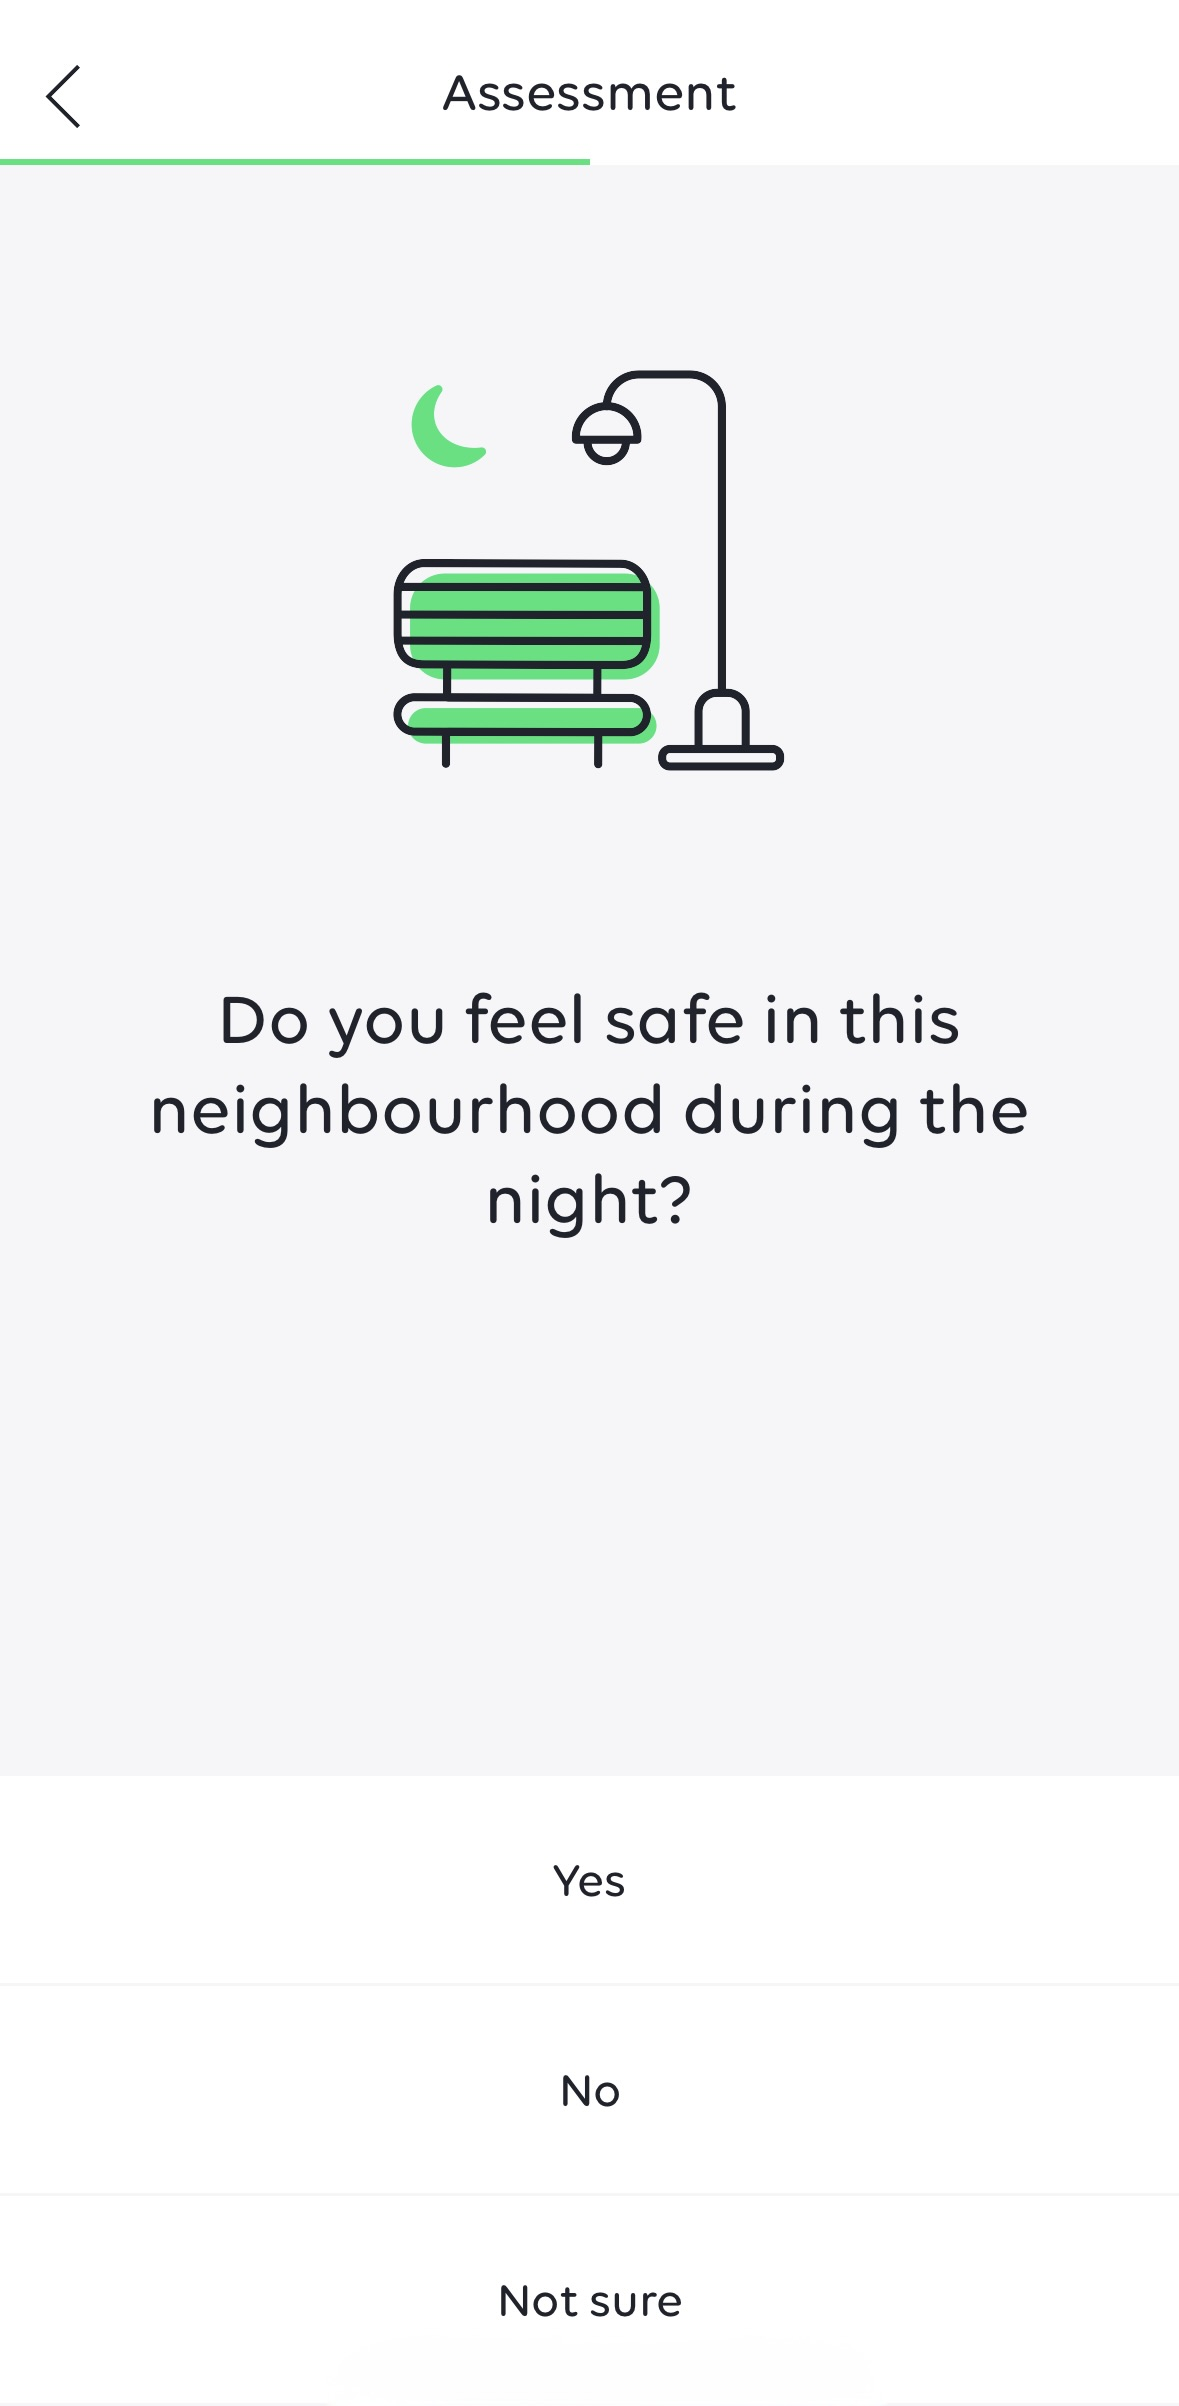
\includegraphics[width=0.5\textwidth]{Arbeit/images/urban_mind01.jpeg}
    \caption{Screenshot einer typischen Frageseite aus der Urban Mind-App}
    \label{fig:urban_mind_screenshot_1}
\end{figure}

Im Gegensatz zu traditionellen querschnittlichen Designs erlaubt das Urban Mind-Tool explizit die Analyse unmittelbarer und zeitverzögerter Effekte (Lag-Effekte). So konnten beispielsweise signifikant positive Effekte von Naturelementen wie Vogelgesang oder dem Sehen von Bäumen auf das momentane Wohlbefinden nachgewiesen werden, welche auch mehrere Stunden nach dem eigentlichen Naturkontakt noch messbar waren \parencite{bakolisUrbanMindUsing2018}. Darüber hinaus betont das Tool die Bedeutung individueller Differenzen und psychologischer Charakteristika, wie beispielsweise Impulsivität, die sich als moderierende Variable herausstellte: Personen mit höherer Impulsivität, welche typischerweise ein erhöhtes Risiko für psychische Erkrankungen aufweisen, profitieren stärker von unmittelbaren Naturerfahrungen.

Hinsichtlich des Designs und der Bedienbarkeit überzeugt die Urban Mind-App durch eine intuitive grafische Gestaltung sowie durch motivierende Elemente wie eine visuelle Übersicht über ausgefüllte und verpasste Fragebögen. Zudem ermöglicht sie Nutzer\:innen, ihre eigenen Daten retrospektiv aufzubereiten, was zu einer angeleiteten Reflexion des eigenen Wohlbefindens beiträgt. Dieses Feature unterstützt insbesondere eine nachhaltige und motivierte Teilnahme über den gesamten Erhebungszeitraum hinweg.

Obwohl Urban Mind zahlreiche methodische und technische Stärken aufweist, berücksichtigt es intersektionale Perspektiven bisher nicht explizit. So sind beispielsweise soziale Kategorien wie Geschlecht, Ethnizität oder sozioökonomischer Status zwar als demografische Variablen erfasst, werden jedoch nicht systematisch in einer intersektionalen Analyse miteinander in Beziehung gesetzt. Theoretisch wäre es möglich, intersektionale Analysen retrospektiv auf Grundlage der erhobenen Daten durchzuführen, eine solche methodische Perspektive wurde jedoch bislang nicht verfolgt.

Die im Rahmen dieser Bachelorarbeit entwickelte App teilt grundlegende methodische Prinzipien mit dem Urban Mind-Tool, wie insbesondere die Nutzung der \gls{ema}-Methode zur Echtzeiterhebung und die Integration räumlicher Kontextinformationen. Im Unterschied zu Urban Mind beinhaltet die entwickelte App jedoch zusätzliche methodische Elemente, wie etwa differenzierte Slider-Fragen, die eine feinere Abstufung subjektiver Empfindungen ermöglichen. Ferner sieht das methodische Konzept dieser Arbeit explizit eine intersektionale Auswertung vor, welche die Urban Mind-Studien in ihrer bisherigen Form nicht integriert haben.

Zusammenfassend lässt sich feststellen, dass Urban Mind in technischer und methodischer Hinsicht ein bewährtes und umfassend validiertes Tool darstellt, dessen methodische Grundprinzipien auch im Rahmen der hier vorliegenden Studie genutzt wurden. Gleichzeitig erweitert die vorliegende Arbeit diesen Ansatz um eine explizit intersektionale Perspektive, welche bisher im Kontext von Echtzeiterhebungen zu räumlichem Wohlbefinden noch unzureichend repräsentiert ist.

Zur Veranschaulichung und besseren Verständlichkeit der methodischen Unterschiede werden im Folgenden ausgewählte Screenshots der Urban Mind-App eingefügt (siehe \Cref{fig:urban_mind_screenshot_1} und Y). Diese zeigen exemplarisch die visuelle Gestaltung der Fragen sowie die ansprechende Übersicht der Teilnehmer\:innen über ihre beantworteten und verpassten Befragungseinheiten, welche als besonders motivierendes Element hervorzuheben sind \parencite{bakolisUrbanMindUsing2018}.

Dieser Vergleich verdeutlicht sowohl methodische Gemeinsamkeiten als auch Unterschiede zwischen den beiden Instrumenten und ermöglicht eine fundierte Einordnung der vorliegenden Studie innerhalb aktueller Ansätze zur Echtzeiterhebung von Wohlbefinden in urbanen Kontexten.


\subsubsection{Tool B: Retrospektive Erhebung und intersektionale Analyse mittels Relief Maps+}

Im Gegensatz zur App „Urban Mind“, die auf eine Echtzeit-Erfassung unmittelbarer Umgebungseinflüsse auf das mentale Wohlbefinden fokussiert, verfolgt das Tool „Relief Maps+“ von Rodó-de-Zárate und Kolleg\*innen einen retrospektiven, explizit intersektionalen Ansatz zur Analyse subjektiver Erfahrungen in unterschiedlichen Räumen und sozialen Kontexten. „Relief Maps+“ ist eine digitale Weiterentwicklung der ursprünglichen „Relief Maps“, die bereits 2014 von Rodó-de-Zárate als empirisches Werkzeug entwickelt wurden, um räumliche, soziale und emotionale Dimensionen intersektionaler Ungleichheiten qualitativ und quantitativ sichtbar zu machen\footnote{Siehe \url{https://reliefmaps.upf.edu/}} \parencite{rodo-de-zarateDevelopingGeographiesIntersectionality2014, luizdesouzaSpiralValidationProcess2025}.

Ziel der „Relief Maps+“ ist es, differenzierte Erfahrungen von Diskriminierung, Unterdrückung, aber auch Privilegien sichtbar zu machen, indem sie drei miteinander verwobene Dimensionen abbilden: die geografische Dimension (konkrete Orte oder räumliche Kontexte), die soziale Dimension (intersektionale Positionierungen wie Gender, Sexualität, Ethnizität oder Alter) und die emotionale Dimension (die subjektiven Gefühle der Teilnehmenden, z. B. Komfort oder Diskomfort). Dadurch werden Machtverhältnisse und deren Auswirkungen auf alltägliche Erfahrungen sowohl räumlich als auch sozial differenziert und emotional nachvollziehbar dargestellt \parencite{rodo-de-zarateIntersectionalitySpatialityEmotions2023}.

Im methodischen Vorgehen erfolgt die Datenerhebung retrospektiv durch ein Online-Formular, in dem die Teilnehmenden ihre subjektiven Erfahrungen in unterschiedlichen sozialen Situationen und an verschiedenen Orten beschreiben. Dabei bewerten sie explizit ihr emotionales Erleben, beispielsweise anhand einer Skala von Komfort zu Diskomfort, und ordnen diese Erfahrungen verschiedenen intersektionalen Positionen (z. B. Geschlecht, Sexualität oder Ethnizität) zu. Daraus resultieren sogenannte „Relief Maps“, die visuell darstellen, an welchen Orten und unter welchen sozialen Bedingungen Diskriminierung oder Privilegierung erlebt wurde \parencite{luizdesouzaSpiralValidationProcess2025, rodo-de-zarateIntersectionalitySpatialityEmotions2023}.

Ein wichtiger Vorteil dieses Ansatzes ist die bewusste und explizite Integration von Reflexivität und Positionalität, da Teilnehmende aufgefordert werden, ihre Erfahrungen in Bezug zu ihren eigenen sozialen Positionierungen kritisch zu reflektieren. „Relief Maps+“ wurde überdies durch ein umfassendes Validierungsverfahren entwickelt, das qualitative, feministische und intersektionale Perspektiven konsequent integrierte. Dabei spielten iterative Feedbackprozesse, Diskussionsgruppen und Pilotstudien eine entscheidende Rolle, um eine ethisch fundierte und theoretisch konsistente Methodik zu gewährleisten \parencite{luizdesouzaSpiralValidationProcess2025}.

Zentraler Aspekt der theoretischen Fundierung von „Relief Maps+“ ist zudem die differenzierte Betrachtung von Emotionen im Zusammenhang mit intersektionalen Ungleichheiten. Gemäss Rodó-de-Zárate fungieren Emotionen als Indikatoren für soziale Positionierungen und Machtverhältnisse, wobei zwischen systematischen Diskomforts, situativen Diskomforts sowie ethischen Diskomforts unterschieden wird. Diese emotionale Perspektive erlaubt es, die komplexen Wechselwirkungen von Orten, sozialen Identitäten und emotionalen Erfahrungen methodisch erfassbar und theoretisch interpretierbar zu machen \parencite{rodo-de-zarateIntersectionalitySpatialityEmotions2023}.

In der Visualisierung der Ergebnisse ermöglichen „Relief Maps+“ die Darstellung von Erfahrungen sowohl individueller als auch gruppenbezogener Art. Die Karten veranschaulichen, wie bestimmte soziale Positionierungen, etwa Geschlecht oder Sexualität, in spezifischen Kontexten systematisch mit Diskriminierung oder Privilegien verbunden sind. Besonders hervorzuheben ist dabei die Fähigkeit des Tools, simultan mehrere Achsen der Unterdrückung und deren räumlich-emotionale Variabilität sichtbar zu machen \parencite{rodo-de-zarateDevelopingGeographiesIntersectionality2014}.

Verglichen mit dem Tool „Urban Mind“ stellt „Relief Maps+“ somit eine tiefer gehende und differenziertere Methodik dar, um intersektionale Dynamiken retrospektiv sichtbar zu machen. Während „Urban Mind“ primär auf unmittelbare Umwelteinflüsse fokussiert und dabei soziale Positionierungen weitgehend unberücksichtigt lässt, setzt „Relief Maps+“ explizit auf eine komplexe intersektionale Perspektive, um systemische und strukturelle Ungleichheiten sichtbar zu machen. Der retrospektive Ansatz erlaubt dabei eine gründliche Reflexion der eigenen Erfahrungen und der sie prägenden gesellschaftlichen Strukturen, bietet allerdings nicht die hohe ökologische Validität und unmittelbare Reaktivität von Echtzeit-Ansätzen wie bei „Urban Mind“.

Für die vorliegende Studie bedeutet dies, dass beide Tools wichtige Anregungen bieten, jedoch unterschiedliche Stärken aufweisen: „Urban Mind“ durch den unmittelbaren, ökologisch validen Zugang zu Alltagserfahrungen, „Relief Maps+“ durch die explizite Integration komplexer intersektionaler Zusammenhänge und deren theoretisch fundierte, räumlich-emotionale Analyse. Beide Perspektiven ergänzen sich methodisch und analytisch, wodurch ein tiefergehendes Verständnis des räumlich situierten, intersektionalen Wohlbefindens erreicht werden kann.


\subsubsection{Einordnung des eigenen Ansatzes}

Die vorliegend entwickelte App greift das Grundprinzip von \emph{Urban Mind} – die mehrfach tägliche Erhebung subjektiver Befindlichkeiten \emph{in situ} – auf und erweitert es in zwei zentralen Punkten:

\begin{enumerate}
    \item \textbf{Methodische Flexibilität.} Neben Single- und Multiple-Choice-Items stehen kontinuierliche Schieberegler sowie optionale Freitextfelder zur Verfügung. Dadurch lassen sich sowohl feingranulare quantitative Einschätzungen als auch kontextspezifische qualitative Informationen erfassen. Die zugrunde liegende React-Native-Codebasis ist modular aufgebaut; neue Fragetypen können mit minimalem Programmieraufwand ergänzt werden.

    \item \textbf{Explizit intersektionale Ausrichtung.} Während \emph{Urban Mind} soziale Kategorien lediglich in der Baseline erfasst, verknüpft der hier gewählte Ansatz zwei Ebenen systematisch: \textit{(i)} detaillierte, einmalig erhobene Soziodemografie (Alter, zugewiesenes und selbstidentifiziertes Geschlecht, sexuelle Orientierung, Behinderung, Einkommen u.\,a.) und \textit{(ii)} situative EMA-Items, die gezielt nach etwaigen Einflüssen eben dieser Merkmale auf das aktuelle Wohlbefinden fragen. Damit wird Intersektionalität nicht nur retrospektiv–korrelativ, sondern \emph{situativ-explizit} operationalisiert.
\end{enumerate}

Die Kombination beider Ebenen erlaubt eine mehrdimensionale Modellierung: Baseline-Merkmale definieren strukturelle Ausgangspositionen, situative Angaben erfassen konkrete Erfahrungen. Durch lineare Mixed-Models oder MAIHDA-Ansätze lassen sich Wechselwirkungen zwischen sozialen Positionen, räumlichen Kontexten und momentanen Befindlichkeiten quantitativ abbilden; Freitextangaben liefern zugleich reichhaltiges Material für eine kontextualisierende, qualitative Vertiefung.

\subsection{Entwicklung der App \textit{InterMind}}

\subsubsection{Ziele und Rahmenbedingungen}

Die zentrale Erhebungslogik der vorliegenden Arbeit basiert auf wiederholten, geolokalisierten Erhebungen zum situativ-affektiven Wohlbefinden der Teilnehmenden. Daraus resultieren spezifische Anforderungen an das digitale Instrument, mit dem diese Daten erfasst werden sollen. Ein geeignetes Erhebungstool muss insbesondere folgende Kriterien erfüllen: Es soll mobil und einfach nutzbar sein, situative Antworten unmittelbar im Alltag der Teilnehmenden ermöglichen, dabei Standortdaten automatisch erfassen und gleichzeitig datenschutzrechtliche sowie technische Hürden für die Nutzer\genderstern innen minimieren. Darüber hinaus war es von Beginn an wichtig, dass das System flexibel und nachhaltig konzipiert ist, um auch über die aktuelle Studie hinaus für zukünftige Forschungsvorhaben eingesetzt werden zu können. Konkret bedeutet dies, dass die Fragenkataloge sowie die Inhalte der App einfach austauschbar und an neue Forschungsfragen oder Zielgruppen anpassbar sein sollten.

Bereits verfügbare Lösungen erfüllten diese Anforderungen nur teilweise oder gar nicht. Kommerzielle Angebote, wie beispielsweise die Forschungsplattform Avicenna\footnote{\href{https://avicennaresearch.com/}{https://avicennaresearch.com/}}, waren aufgrund hoher Lizenzkosten für eine studentische Abschlussarbeit nicht praktikabel. Zudem erlauben solche Dienste in der Regel keine vollständige Kontrolle über die verarbeiteten Daten und bieten nur begrenzte Anpassungsmöglichkeiten hinsichtlich Fragenstruktur und Datenerfassung. Auf der anderen Seite stehen Apps wie Urban Mind\footnote{\href{https://urbanmind.info/}{https://urbanmind.info/}}, die zwar grundsätzlich für \gls{esm}-Erhebungen im Forschungskontext entwickelt wurden, jedoch nicht quelloffen und entsprechend auch nicht eigenständig erweiterbar sind. Gerade im Kontext dieser Studie, bei der sensible Daten zu Wohlbefinden und sozialen Zugehörigkeiten erhoben werden, ist eine transparente und unabhängige Kontrolle der Datenerhebung jedoch von besonderer Bedeutung.

Vor diesem Hintergrund wurde das Ziel formuliert, eine eigene digitale Anwendung zu entwickeln, die bewusst quelloffen und modular gestaltet ist. Diese \gls{opensource}-Architektur sollte es ermöglichen, die gesamte Datenverarbeitung transparent und nachvollziehbar zu gestalten sowie künftige Anpassungen unkompliziert vorzunehmen. Aufgrund der limitierten zeitlichen Ressourcen innerhalb der Bachelorarbeit wurde darüber hinaus darauf geachtet, weit verbreitete Technologien und Frameworks zu wählen, um die Entwicklung möglichst effizient, wartungsarm und für Dritte nachvollziehbar zu halten.

\subsubsection{Konzeptionsphase}
Auf Basis der beschriebenen Anforderungen wurde zunächst ein detaillierter Anforderungskatalog entwickelt, der als zentraler Leitfaden für die weiteren Schritte der App-Entwicklung diente. Dieser Katalog wurde iterativ ergänzt, konkretisiert und während des gesamten Entwicklungsprozesses kontinuierlich an methodische und technische Erkenntnisse angepasst. In Anlehnung an etablierte Konzepte aus der Softwareentwicklung wurde dabei zwischen funktionalen und nicht-funktionalen Anforderungen unterschieden.

Funktionale Anforderungen definieren dabei konkret, \textit{was} die App im praktischen Einsatz leisten muss, und legen somit die notwendigen Funktionen und Abläufe der Anwendung fest. Für diese Studie bedeutete dies insbesondere, dass die App den Teilnehmenden täglich drei zufällig über den Tag verteilte Beantwortungszeiträume von einer Stunde ermittelt und jeweils zum Start dieser Zeiträume \glspl{pushnotification} sendet. Weiter wurde festgelegt, dass bei jeder erfolgten Befragung der aktuelle Standort automatisiert mit erfasst werden soll, sofern die Teilnehmenden dies technisch erlauben. Um die Erhebung flexibel und bedarfsgerecht zu gestalten, wurden zudem verschiedene Fragetypen vorgesehen, darunter Single-Choice, Multiple-Choice, Skalen-basierte Fragen (Slider) sowie Freitextfelder. Schliesslich wurde es als zwingende funktionale Anforderung definiert, dass Teilnehmende jederzeit eigenständig sämtliche gespeicherten Daten löschen können. Die Teilnahme erfolgt dabei vollständig anonym, über eine gerätegebundene, automatisch generierte pseudonyme \gls{uuid}, ohne jegliche Form der Registrierung oder der Eingabe personenbezogener Daten.

Nicht-funktionale Anforderungen legen hingegen fest, \textit{wie} diese Funktionen umgesetzt werden sollen, und beschreiben qualitative Merkmale wie Sicherheit, Benutzerfreundlichkeit oder technische Kompatibilität. In diesem Projekt wurden insbesondere Datenschutz und Datensicherheit als zentrale nicht-funktionale Anforderungen definiert. Sämtliche Datenverarbeitungsprozesse mussten entsprechend den Vorgaben des \acrfull{dsg} und der Europäischen Datenschutzgrundverordnung \acrshort{dsgvo} erfolgen. Weiterhin wurde Mehrsprachigkeit (Deutsch, Englisch und Französisch) als Voraussetzung formuliert, ebenso wie die Möglichkeit einer späteren Erweiterung auf weitere Sprachen. Darüber hinaus sollte die App ursprünglich grundsätzlich offlinefähig sein. Im laufe der Entwicklung wurde diese Anforderung jedoch aufgegeben, da das dazu geführt hätte, dass jede Änderung im Fragenkatalog ein Update der App und anschliessend je nachdem nicht kompatible Versionen der App entstünden. Um Teilnehmenden mit unterschiedlichen Mobilgeräten die Teilnahme möglichst einfach zu machen, war zudem eine plattformübergreifende Kompatibilität für iOS und Android erforderlich. Aus wissenschaftlicher Sicht war schliesslich eine offene, modulare und nachvollziehbare Codebasis wichtig, sodass Anpassungen und Erweiterungen des Systems durch andere Forschende mit minimalem Aufwand möglich bleiben. Dies wurde dadurch erreicht, dass die App als \gls{opensource}-Projekt auf Github\footnote{\href{https://github.com/lbatschelet/intermind}{https://github.com/lbatschelet/intermind}} veröffentlicht wurde.

Die Priorisierung und Auswahl dieser Anforderungen erfolgte unter Berücksichtigung der konkreten Forschungsziele, der vorhandenen Literatur zu mobilen Anwendungen im Bereich \gls{esm} \parencite{chenPerceivedUrbanEnvironment2025, randallDevelopmentTrialMobile2013}, datenschutzrechtlicher Vorgaben sowie praktischer Erfahrungen aus dem eigenen Informatikstudium. Aufgrund des iterativen Vorgehens während der Entwicklung kam es dabei auch später immer wieder zu Anpassungen und Nachjustierungen einzelner Anforderungen – etwa wenn Rückmeldungen aus ersten Testläufen zu veränderten Schwerpunkten führten oder technische Herausforderungen eine Neuausrichtung bestimmter Anforderungen notwendig machten.

\subsubsection{Implementierung}

Für die technische Umsetzung der zuvor definierten Anforderungen wurde als zentrale Entwicklungsumgebung das \gls{framework} \gls{reactnative} in Kombination mit der Entwicklungsplattform \gls{expo} gewählt. Diese Entscheidung ermöglichte es, mit einer einheitlichen Codebasis sowohl iOS- als auch Android-Geräte zu unterstützen, wodurch nicht nur der Entwicklungsaufwand reduziert, sondern auch eine konsistente und vergleichbare Benutzererfahrung auf beiden Plattformen gewährleistet werden konnte. Als serverseitige Infrastruktur wurde \gls{supabase} eingesetzt – ein quelloffenes \gls{backend}-as-a-Service auf Basis einer relationalen \gls{postgresql}-\gls{datenbank}, die Authentifizierung, Datenspeicherung und sichere Datenübertragung integriert bereitstellt.

Beim ersten Start der App generiert das System automatisch eine eindeutige, nicht rückverfolgbare \gls{uuid}, die lokal auf dem Gerät gespeichert wird. Diese \gls{uuid} fungiert als pseudonymisierte Kennung für sämtliche Datenbankoperationen und ersetzt jegliche Form der persönlichen Registrierung. Der eigentliche Fragenkatalog wurde bewusst nicht direkt im Programmcode der App hinterlegt, sondern dynamisch über eine \gls{json}-Konfigurationsdatei geladen, die serverseitig auf der \gls{supabase}-Plattform abgelegt ist. Diese Struktur erlaubt es, den Fragenkatalog jederzeit flexibel und ohne ein zusätzliches App-Update zu ändern oder zu erweitern. Die Kehrseite dieser dynamischen Herangehensweise besteht darin, dass die App zum Laden der Befragungsinhalte auf eine bestehende Internetverbindung angewiesen ist.

Die Zeitpunkte der täglichen Befragungen werden automatisch nach Abschluss des ersten Fragebogens berechnet und anschliessend lokal auf dem Gerät der Teilnehmenden eingeplant. An jedem dieser Slots haben die teilnehmendenden eine Stunde Zeit die Befragung auszufüllen. Dadurch konnten ständige serverseitige Abfragen oder Hintergrundprozesse vermieden werden, was sich positiv auf die Akkulaufzeit und den Datenverbrauch der Geräte auswirkte. Die technische Herausforderung bestand darin, eine zuverlässige und plattformübergreifend kompatible Lösung zur lokalen Planung der \glspl{pushnotification} zu entwickeln, da sich die mobilen Betriebssysteme (iOS und Android) teilweise erheblich in der Handhabung von Hintergrundprozessen unterscheiden.

Das \gls{frontend} der App ist bewusst freundlich und minimalistisch gestaltet, um eine intuitive Nutzung zu gewährleisten und gleichzeitig eine neutrale und unvoreingenommene Wahrnehmung der Fragen sicherzustellen. Die Benutzerführung ist in drei zentrale Bereiche gegliedert: einen Startbildschirm, der den nächstmöglichen Beantwortungszeitraum anzeigt, einen separaten Bereich für den eigentlichen Fragebogen sowie einen Informations- und Einstellungsbildschirm, auf dem umfassende Hinweise zur Befragung und zum Datenschutz hinterlegt sind.

Die Implementierung technischer Anforderungen, wie etwa die Verwaltung von Systemberechtigungen (z. B. Standortfreigabe oder Push-Benachrichtigungen), erfolgte mithilfe von standardisierten Expo-Modulen. Dies vereinfachte viele dieser technischen Herausforderungen erheblich. Hingegen erwies sich die Qualitätssicherung im Laufe des Entwicklungsprozesses als aufwändiger, da keine automatisierte Testsuite implementiert wurde. Fehler wurden daher während der Entwicklung stets manuell identifiziert und behoben. Obwohl dieses Vorgehen im Rahmen der begrenzten zeitlichen Ressourcen pragmatisch war, führte es insgesamt zu einem erhöhten Arbeitsaufwand und erschwerte die systematische und nachhaltige Überprüfung der Softwarequalität.

\subsubsection{Datenschutz und Sicherheit}
Datenschutzaspekte waren von Beginn an zentrale Bestandteile des Entwicklungsprozesses und prägten massgeblich die technische und methodische Umsetzung der App. Dabei wurde konsequent dem Prinzip Privacy by Design gefolgt, welches vorsieht, dass Datenschutzanforderungen bereits bei der Konzeption einer Anwendung berücksichtigt und nicht nachträglich integriert werden. Ziel war es, durch entsprechende technische und organisatorische Massnahmen ein höchstmögliches Mass an Privatsphäre für die Teilnehmenden sicherzustellen sowie gleichzeitig volle Transparenz über die Datenerhebung und -verarbeitung zu gewährleisten.

Die Teilnahme erfolgt ausschliesslich anonymisiert über eine automatisch generierte, gerätegebundene UUID (Universally Unique Identifier). Diese UUID ersetzt vollständig eine Registrierung oder Angabe persönlicher Informationen wie Name, Telefonnummer oder E-Mail-Adresse. Standortdaten werden jeweils ausschliesslich zum Zeitpunkt der Befragung erfasst, eine kontinuierliche Standortverfolgung findet nicht statt. Sämtliche erhobenen Daten – darunter demografische Angaben, situativ-affektives Wohlbefinden, Angaben zur Umgebung und der zum Zeitpunkt der Befragung ermittelte Standort – werden in pseudonymisierter Form auf einem Server in der Schweiz gespeichert.

Als technologische Grundlage für die Datenspeicherung dient die zuvor genannte \gls{supabase}-Plattform mit einer \gls{postgresql}-\gls{datenbank}. Dabei wird eine Zugriffssteuerung auf Zeilenebene \gls{rls} verwendet, um sicherzustellen, dass jedes Endgerät ausschliesslich auf seine eigenen Daten zugreifen kann. Diese technische Massnahme verhindert zuverlässig unberechtigte Zugriffe auf fremde Datensätze. Zudem erfolgt die gesamte Datenübertragung zwischen Endgerät und Server verschlüsselt und über authentifizierte Schnittstellen.

Die Teilnehmenden behalten dabei stets die volle Kontrolle über ihre Daten: Über eine integrierte Funktion innerhalb der App können sämtliche eigenen Datensätze jederzeit selbstständig gelöscht werden. Dies führt zu einer vollständigen und unwiderruflichen Entfernung aller mit der entsprechenden \gls{uuid} verknüpften Daten aus der \gls{datenbank}. Somit liegt die vollständige Kontrolle über die Datenspeicherung zu jedem Zeitpunkt bei den Teilnehmenden selbst.

Alle datenschutzrechtlichen Aspekte, einschliesslich der konkreten Umsetzung der genannten technischen und organisatorischen Massnahmen, sind transparent in einer umfassenden Datenschutzrichtlinie dokumentiert. Diese Datenschutzrichtlinie ist sowohl über die App selbst abrufbar als auch öffentlich über die eigens eingerichtete Website\footnote{\href{https://intermind.ch/privacy-policy.html}{https://intermind.ch/privacy-policy.html}} zugänglich. Darin werden zudem die Rechte der Teilnehmenden gemäss dem \gls{dsg} umfassend dargestellt.

\subsubsection{Test und Iteration}
Zur Sicherstellung der technischen Zuverlässigkeit sowie der Gebrauchstauglichkeit der App wurde im Rahmen dieser Arbeit ein zweistufiger Testprozess durchgeführt. Aufgrund der begrenzten Ressourcen und des Projektumfangs kam dabei keine strukturierte automatisierte Testsuite zum Einsatz. Stattdessen wurde ein pragmatischer Ansatz gewählt, bei dem auftretende Probleme laufend manuell identifiziert und unmittelbar behoben wurden. Obwohl diese Vorgehensweise zu einer insgesamt soliden Funktionalität der Anwendung führte, erwies sich die fehlende automatisierte Qualitätssicherung im Entwicklungsprozess wiederholt als Herausforderung und führte zu einem insgesamt höheren zeitlichen Aufwand bei der Fehlersuche.

In einer ersten Phase fanden fortlaufende technische Funktionstests während der Implementierung statt. Im Fokus dieser Tests standen insbesondere die korrekte Verarbeitung des dynamisch geladenen Fragenkatalogs (\gls{json}-Datei), die fehlerfreie Übertragung von Daten an das \gls{supabase}-\gls{backend}, das Verhalten der App bei unterbrochener oder unzuverlässiger Internetverbindung sowie die plattformübergreifende Zuverlässigkeit der lokalen Planung und Ausführung von \glspl{pushnotification}. Da sich iOS und Android in ihrer Handhabung von Hintergrundprozessen, Benachrichtigungssystemen und Berechtigungsanfragen teilweise stark unterscheiden, wurde der Funktionsumfang regelmässig auf verschiedenen Geräten mit unterschiedlichen Betriebssystemversionen manuell geprüft.

In der zweiten Phase wurde ein interner Pretest mit vier Personen durchgeführt, welche die App über einen Zeitraum von zwei Wochen nutzten. Die Teilnehmenden erhielten hierzu über die offiziellen Beta-Testplattformen (TestFlight für iOS und Google Play Console für Android) Zugang zur Anwendung. Dabei wurden gezielte Aufgaben gestellt, um spezifische technische und inhaltliche Aspekte zu überprüfen sowie allgemeines Feedback zur Benutzerfreundlichkeit und Verständlichkeit der Fragen zu sammeln. Die Rückmeldungen der Testpersonen bezogen sich vor allem auf die Klarheit und Lesbarkeit einzelner Fragen und Texte, auf kleinere Probleme bei der erstmaligen Vergabe von App-Berechtigungen (z. B. Standortzugriff), sowie auf Darstellungsprobleme bestimmter \gls{ui}-Elemente auf verschiedenen Geräten.

Die Ergebnisse aus dieser Testphase führten sowohl zu technischen Anpassungen als auch zu inhaltlichen Änderungen im Fragebogen. Mehrere Fragen wurden sprachlich präzisiert oder gekürzt, einzelne Items wurden ganz gestrichen. Weiterhin wurden Anpassungen an der Benutzeroberfläche vorgenommen, beispielsweise bei Abständen und der Platzierung von Slider-Beschriftungen. Aufgrund der fehlenden automatisierten Tests erforderte jede Änderung erneut eine manuelle Überprüfung der gesamten Funktionalität, was insgesamt erheblichen zusätzlichen Aufwand bedeutete.

Insgesamt ermöglichte der iterative Testprozess jedoch, wesentliche Schwachstellen vor dem Beginn der eigentlichen Datenerhebung zu identifizieren und zu beheben. Obwohl auf eine formalisierte Usability-Evaluation verzichtet wurde, konnten durch diese Vorgehensweise zentrale technische sowie benutzerorientierte Probleme effektiv adressiert werden.

\subsubsection{Veröffentlichung und Distribution}

Um die entwickelte App für die eigentliche Datenerhebung nutzen zu können, wurde eine Veröffentlichung über die offiziellen App-Stores von Apple (iOS) und Google (Android) angestrebt. Beide Plattformen stellen dabei unterschiedliche technische, administrative und finanzielle Anforderungen, die den Veröffentlichungsprozess massgeblich beeinflussten.

Die Veröffentlichung im Apple App Store setzte zunächst den Erwerb einer kostenpflichtigen Entwicklerlizenz voraus, für die eine jährliche Gebühr von CHF 100 zu entrichten war. Nach erfolgreicher Einrichtung dieses Entwicklerkontos wurde die App zur Veröffentlichung eingereicht, allerdings von Apple zunächst nicht für eine finale Veröffentlichung im regulären App Store zugelassen. Als Begründung wurde angegeben, die App weise zu wenig inhaltlichen Mehrwert auf – eine Entscheidung, die aus Sicht der Entwicklung nur schwer nachvollziehbar war. Der Prüfprozess bei Apple ist zum Zeitpunkt des Abschlusses dieser Arbeit noch nicht vollständig abgeschlossen. Dennoch konnte die App über Apples eigene Plattform für öffentliche Beta-Tests („TestFlight“) bereitgestellt werden, sodass Teilnehmende der Studie über einen offiziellen TestFlight-Link Zugang zur App erhielten.

Im Gegensatz dazu verlangte Google für eine Veröffentlichung im Android Play Store keine laufenden Lizenzkosten. Allerdings stellte Google die Bedingung, dass vor einer offenen Betaversion zunächst ein geschlossener Test mit mindestens 20 Personen über einen Zeitraum von zwei Wochen durchgeführt werden musste. Da es innerhalb des zeitlichen Rahmens dieser Bachelorarbeit nicht möglich war, eine ausreichende Anzahl Testpersonen mit Android-Geräten zu rekrutieren, wurde hierfür ein externer Dienstleister in Anspruch genommen, welcher diesen erforderlichen Test für eine Gebühr von CHF 30 durchführte. Nach erfolgreichem Abschluss dieses Tests wurde die App im Play Store als offene Beta veröffentlicht und war somit öffentlich verfügbar.

Darüber hinaus verlangten beide Plattformen, dass eine öffentlich zugängliche Datenschutzrichtlinie zur Verfügung steht. Zu diesem Zweck wurde die Website intermind.ch eingerichtet, auf der neben der vollständigen Datenschutzerklärung auch ergänzende Informationen zum Forschungshintergrund abrufbar sind. Die Kosten hierfür beliefen sich auf einmalig CHF 10 für die Domainregistrierung; Hosting-Kosten entstanden keine zusätzlichen, da auf bereits bestehende Infrastruktur zurückgegriffen wurde.

Durch die Veröffentlichung über offizielle App-Plattformen konnten technische Hürden für die Teilnehmenden minimiert und zugleich plattformspezifische Anforderungen (beispielsweise hinsichtlich Datenschutzrichtlinien und Update-Management) zuverlässig erfüllt werden. Trotz vereinzelter Schwierigkeiten im Freigabeprozess ermöglichte dieses Vorgehen letztlich eine unkomplizierte Distribution und Nutzung der Anwendung im Rahmen dieser Arbeit.

\subsection{Fragebogenstruktur und Operationalisierung}

Der Fragebogen besteht aus zwei zentralen Elementen:

\paragraph{Baseline-Befragung (einmalig):}
Hier wurden grundlegende demografische Variablen (Alter, Geschlecht, sexuelle Orientierung, Behinderung, sozioökonomischer Hintergrund) erhoben, um soziale Positionierungen für spätere intersektionale Analysen verfügbar zu machen. Fragen wurden bewusst offen oder mit freier Spezifikation gestaltet, um Normativität in den Antwortoptionen zu vermeiden und soziale Positionierungen differenziert erfassen zu können.

\paragraph{Situative Befragung (wiederholt):}
Der wiederholt eingesetzte Fragebogen besteht aus kurzen situativen Erhebungen, die mittels EMA durchgeführt wurden. Teilnehmer:innen wurden regelmässig aufgefordert, Fragen zu ihrem momentanen Wohlbefinden (z.\,B. empfundene Sicherheit, Zugehörigkeit, Entspannung) sowie zur aktuellen räumlichen und sozialen Umgebung zu beantworten. Hierbei kamen insbesondere Slider-Fragen zum Einsatz, um eine kontinuierliche Bewertung zu ermöglichen. Ergänzend wurde ein optionales Freitextfeld angeboten, das qualitative Kontextinformationen und subjektive Reflexionen zuliess.

Der Begriff \emph{Operationalisierung} bezeichnet hierbei die konkrete Umsetzung theoretischer Konstrukte in messbare Indikatoren. Wohlbefinden wurde operationalisiert über sieben zentrale Dimensionen (u.\,a. Entspannung, Sicherheit, Zugehörigkeit), die in der Literatur als relevant identifiziert wurden. Räumliche und soziale Kontexte wurden mit Items operationalisiert, die beispielsweise aus der Forschung von Bakolis et al. (2018) übernommen und für die vorliegende Studie adaptiert wurden.

\subsubsection{Ablauf und Durchführung der Datenerhebung}

Die Datenerhebung fand im Rahmen der einführenden Exkursion „Recht auf Stadt“ im ersten Studienjahr des Bachelorstudiengangs Geographie an der Universität Bern im Mai 2025 statt. Die teilnehmenden Studierenden wurden zu Beginn der Exkursion über Zielsetzung und Ablauf informiert und konnten anschliessend freiwillig an der Befragung teilnehmen. Die Nutzung der App wurde über den gesamten Exkursionszeitraum von drei Tagen durchgeführt, wobei die Teilnehmenden via Push-Benachrichtigungen mehrfach täglich aufgefordert wurden, die kurzen situativen Befragungen auszufüllen. Die Baseline-Befragung erfolgte einmalig zu Beginn.

Die Durchführung im Exkursionssetting ermöglichte eine kontrollierte Testung der technischen Funktionalität und eine hohe Compliance bei den Teilnehmenden. Gleichzeitig erlaubte dieses Setting, reale räumliche Kontexte, wie unterschiedliche urbane Umgebungen in Zürich, Basel und Bern, unmittelbar in die Datenerhebung einzubeziehen. Insgesamt zeichneten sich die Daten durch eine hohe räumliche und kontextuelle Varianz aus, die zentrale Grundlage für die späteren intersektionalen Analysen bildete.

Die vollständigen Fragebögen (Baseline- und situative Befragungen) sind als ergänzende Dokumentation digital im GitHub-Repository der App hinterlegt. Dies folgt dem Prinzip offener und transparenter Forschung. Eine detaillierte Fragebogenübersicht kann zusätzlich im Anhang dieser Arbeit eingesehen werden, um die inhaltliche Struktur und die Operationalisierung der theoretischen Konstrukte nachvollziehbar zu machen.

Zusammenfassend stellt die entwickelte App somit ein methodisch differenziertes, technisch flexibles Instrument dar, das sowohl situative Dynamiken als auch intersektionale soziale Strukturen systematisch erfassbar macht. Die enge Verknüpfung mit einem explizit intersektional ausgerichteten Fragebogen ermöglicht es, bestehende methodische Ansätze (Urban Mind, Relief Maps+) gezielt zu erweitern und dabei neue Erkenntnisse zur Beziehung von Raum, Wohlbefinden und sozialer Positionierung zu generieren.


\subsection{Limitationen und Herausforderungen der Datenerhebung}

\subsubsection{Geringe Rücklaufquote und mögliche Ursachen}

\subsubsection{Auswirkungen auf die Datenqualität und Analyse}


\clearpage

\section{«Build your own tools»: Entwicklung der App \textit{InterMind}}
\label{sec:entwicklung_app}

Im Zuge dieser Arbeit wurde die App \textit{InterMind} entwickelt, die als technische Grundlage für wiederholte, geolokalisierte und pseudonymisierte Befragungen dient. Sie bildet die Infrastruktur für anschliessend durchgeführte Pilot-Studie. Die App und der in dieser Arbeit eingesetzte Fragenkatalog wurden parallel und iterativ konzipiert. Während dieser Abschnitt die technische Entwicklung der App dokumentiert, wird die inhaltliche Gestaltung des Fragebogens im \cref{sec:fragebogenentwicklung} erläutert. Der vollständige Quellcode der App ist auf \gls{github}\footnote{\href{https://github.com/lbatschelet/intermind}{https://github.com/lbatschelet/intermind}} veröffentlicht.


\subsection{From scratch – Warum eine eigene App?}

Die zentrale Erhebungslogik der vorliegenden Arbeit basiert auf wiederholten, geolokalisierten Erhebungen zum situativ-affektiven Wohlbefinden der Teilnehmenden. Daraus resultieren spezifische Anforderungen an das Instrument, mit dem diese Daten erfasst werden sollen. Ein geeignetes Erhebungstool muss insbesondere folgende Kriterien erfüllen: Es soll mobil und einfach nutzbar sein, situative Antworten unmittelbar im Alltag der Teilnehmenden ermöglichen, dabei Standortdaten automatisch erfassen und gleichzeitig datenschutzrechtliche sowie technische Hürden für die Nutzer\genderstern innen minimieren. Darüber hinaus war es von Beginn an wichtig, dass das System flexibel und nachhaltig konzipiert ist, um auch für zukünftige Arbeiten eingesetzt werden zu können. Konkret bedeutet dies, dass die Fragenkataloge sowie die Inhalte der App einfach austauschbar und an neue Forschungsfragen oder Zielgruppen anpassbar sein sollten.

Bereits verfügbare Lösungen erfüllten diese Anforderungen nur teilweise oder gar nicht. Kommerzielle Angebote, wie beispielsweise die Marktforschungsplattform Avicenna\footnote{\href{https://avicennaresearch.com/}{https://avicennaresearch.com/}}, sind aufgrund hoher Lizenzkosten für eine studentische Abschlussarbeit nicht praktikabel. Zudem erlauben viele solcher Dienste in keine vollständige Kontrolle über die verarbeiteten Daten und bieten nur begrenzte Anpassungsmöglichkeiten hinsichtlich Fragenstruktur und Datenerfassung. Auf der anderen Seite stehen Apps wie Urban Mind\footnote{\href{https://urbanmind.info/}{https://urbanmind.info/}}, die zwar grundsätzlich für \gls{gema}-Erhebungen im Forschungskontext entwickelt wurden, jedoch nicht quelloffen und entsprechend auch nicht eigenständig erweiterbar sind. Zudem ist mir persönlich in dieser Arbeit bei der sensible Daten zu Wohlbefinden und sozialen Zugehörigkeiten erhoben werden, eine transparente und sichere Datenverarbeitung von besonderer Bedeutung.

Vor diesem Hintergrund wurde das Ziel formuliert, eine eigene digitale Anwendung zu entwickeln, die bewusst quelloffen und modular gestaltet ist. Diese \gls{opensource}-Architektur sollte es ermöglichen, die gesamte Datenverarbeitung transparent und nachvollziehbar zu gestalten sowie künftige Anpassungen unkompliziert vorzunehmen. Aufgrund der limitierten zeitlichen Ressourcen innerhalb der Bachelorarbeit wurde darüber hinaus darauf geachtet, weit verbreitete Technologien und Frameworks zu wählen, um die Entwicklung möglichst effizient, wartungsarm und für Dritte nachvollziehbar zu halten.

\subsection{Konzeption und Anforderungen – Der Weg zur eigenen Infrastruktur}
Auf Basis der beschriebenen Anforderungen wurde zunächst ein detaillierter Anforderungskatalog entwickelt, der als zentraler Leitfaden für die weiteren Schritte der Entwicklung diente. Dieser Katalog wurde iterativ ergänzt, konkretisiert und während des gesamten Entwicklungsprozesses kontinuierlich an methodische und technische Erkenntnisse angepasst. In Anlehnung an etablierte Konzepte aus der Softwareentwicklung wurde dabei zwischen funktionalen und nicht-funktionalen Anforderungen unterschieden.

Funktionale Anforderungen definieren dabei konkret, \textit{was} die App im praktischen Einsatz leisten muss, und legen somit die notwendigen Funktionen und Abläufe der Anwendung fest. Für diese Studie bedeutete dies insbesondere, dass die App den Teilnehmenden täglich drei zufällig über den Tag verteilte Beantwortungszeiträume von einer Stunde ermittelt und jeweils zum Start dieser Zeiträume \glspl{pushnotification} sendet. Diese Anforderung schloss bereits früh eine Browser-basierte Erhebung aus, und führte zum Entscheid eine App-basierte Erhebung zu wählen. Weiter wurde festgelegt, dass bei jeder erfolgten Befragung der aktuelle Standort automatisiert mit erfasst werden soll, sofern die Teilnehmenden dies technisch erlauben. Um die Erhebung flexibel und bedarfsgerecht zu gestalten, wurden zudem verschiedene Fragetypen vorgesehen, darunter Single-Choice, Multiple-Choice, Skalen-basierte Fragen (Slider) sowie Freitextfelder. Schliesslich wurde es als zwingende funktionale Anforderung definiert, dass Teilnehmende jederzeit eigenständig sämtliche gespeicherten Daten löschen können. Die Teilnahme erfolgt dabei vollständig anonym, über eine gerätegebundene, automatisch generierte pseudonyme \gls{uuid}, ohne jegliche Form der Registrierung oder der Eingabe personenbezogener Daten.
 
Nicht-funktionale Anforderungen legen hingegen fest, \textit{wie} diese Funktionen umgesetzt werden sollen, und beschreiben qualitative Merkmale wie Sicherheit, Benutzerfreundlichkeit oder technische Kompatibilität. In diesem Projekt wurden insbesondere Datenschutz und Datensicherheit als zentrale nicht-funktionale Anforderungen definiert. Sämtliche Datenverarbeitungsprozesse müssen entsprechend den Vorgaben des \acrfull{dsg} und der Europäischen Datenschutzgrundverordnung \acrshort{dsgvo} erfolgen. Weiterhin wurde Mehrsprachigkeit (Deutsch, Englisch und Französisch) als Voraussetzung formuliert, ebenso wie die Möglichkeit einer späteren Erweiterung auf weitere Sprachen. Darüber hinaus sollte die Anwendung ursprünglich grundsätzlich offlinefähig sein. Im laufe der Entwicklung wurde diese Anforderung jedoch aufgegeben, da das dazu geführt hätte, dass jede Änderung im Fragenkatalog ein Update der App und anschliessend je nachdem nicht kompatible Versionen der App entstünden. Um Teilnehmenden mit unterschiedlichen Mobilgeräten die Teilnahme möglichst einfach zu machen, war zudem eine plattformübergreifende Kompatibilität für  und Android erforderlich. Schliesslich war eine offene, modulare und nachvollziehbare Codebasis wichtig, sodass Anpassungen und Erweiterungen des Systems durch andere Forschende mit minimalem Aufwand möglich bleiben. Dies wurde dadurch erreicht, dass die App als \gls{opensource}-Projekt auf \gls{github}\footnote{\href{https://github.com/lbatschelet/intermind}{https://github.com/lbatschelet/intermind}} veröffentlicht wurde.

Die Priorisierung und Auswahl dieser Anforderungen erfolgte unter Berücksichtigung der konkreten Forschungsziele, der vorhandenen Literatur zu mobilen Anwendungen im Bereich \gls{esm}/\gls{gema} \parencite[u.a.][]{chenPerceivedUrbanEnvironment2025, bakolisUrbanMindUsing2018, randallDevelopmentTrialMobile2013}, datenschutzrechtlicher Vorgaben sowie praktischer Erfahrungen aus dem eigenen Studium. Aufgrund des iterativen Vorgehens während der Entwicklung kam es dabei auch später immer wieder zu Anpassungen und Nachjustierungen einzelner Anforderungen.

\subsection{Technische Umsetzung – Prinzipien, Praktiken und Kompromisse}

\begin{figure}[h]
    \centering
    \begin{minipage}[t]{0.38\textwidth}
        \centering
        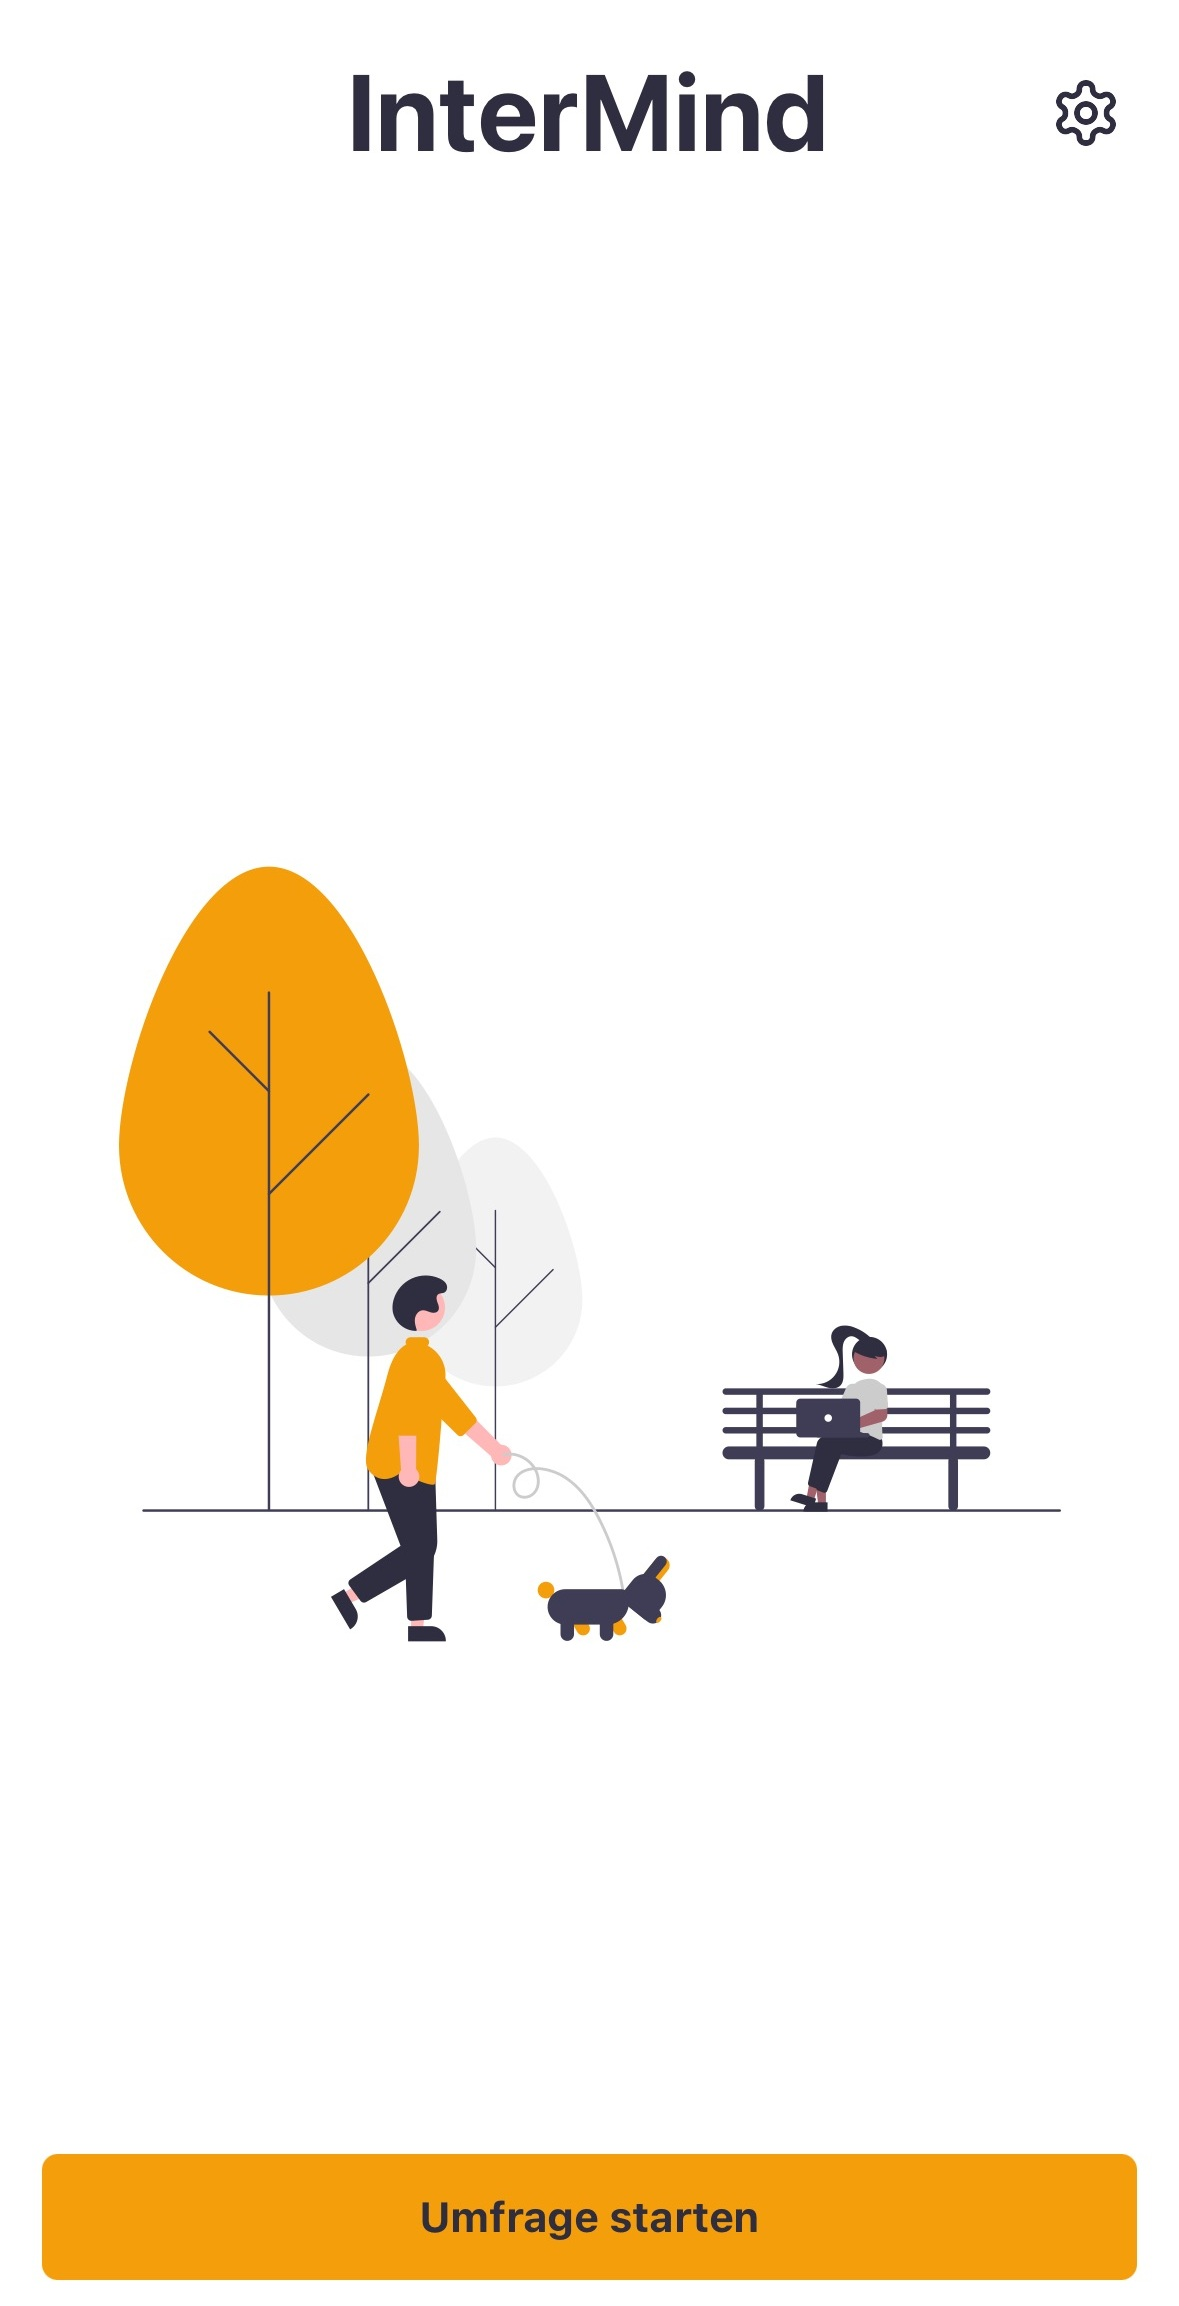
\includegraphics[width=\textwidth]{Arbeit/images/printscreens/startscreen.jpeg}
        \caption{Startbildschirm der App \textit{InterMind}}
        \label{fig:startscreen}
    \end{minipage}
    \hspace{0.1\textwidth}
    \begin{minipage}[t]{0.38\textwidth}
        \centering
        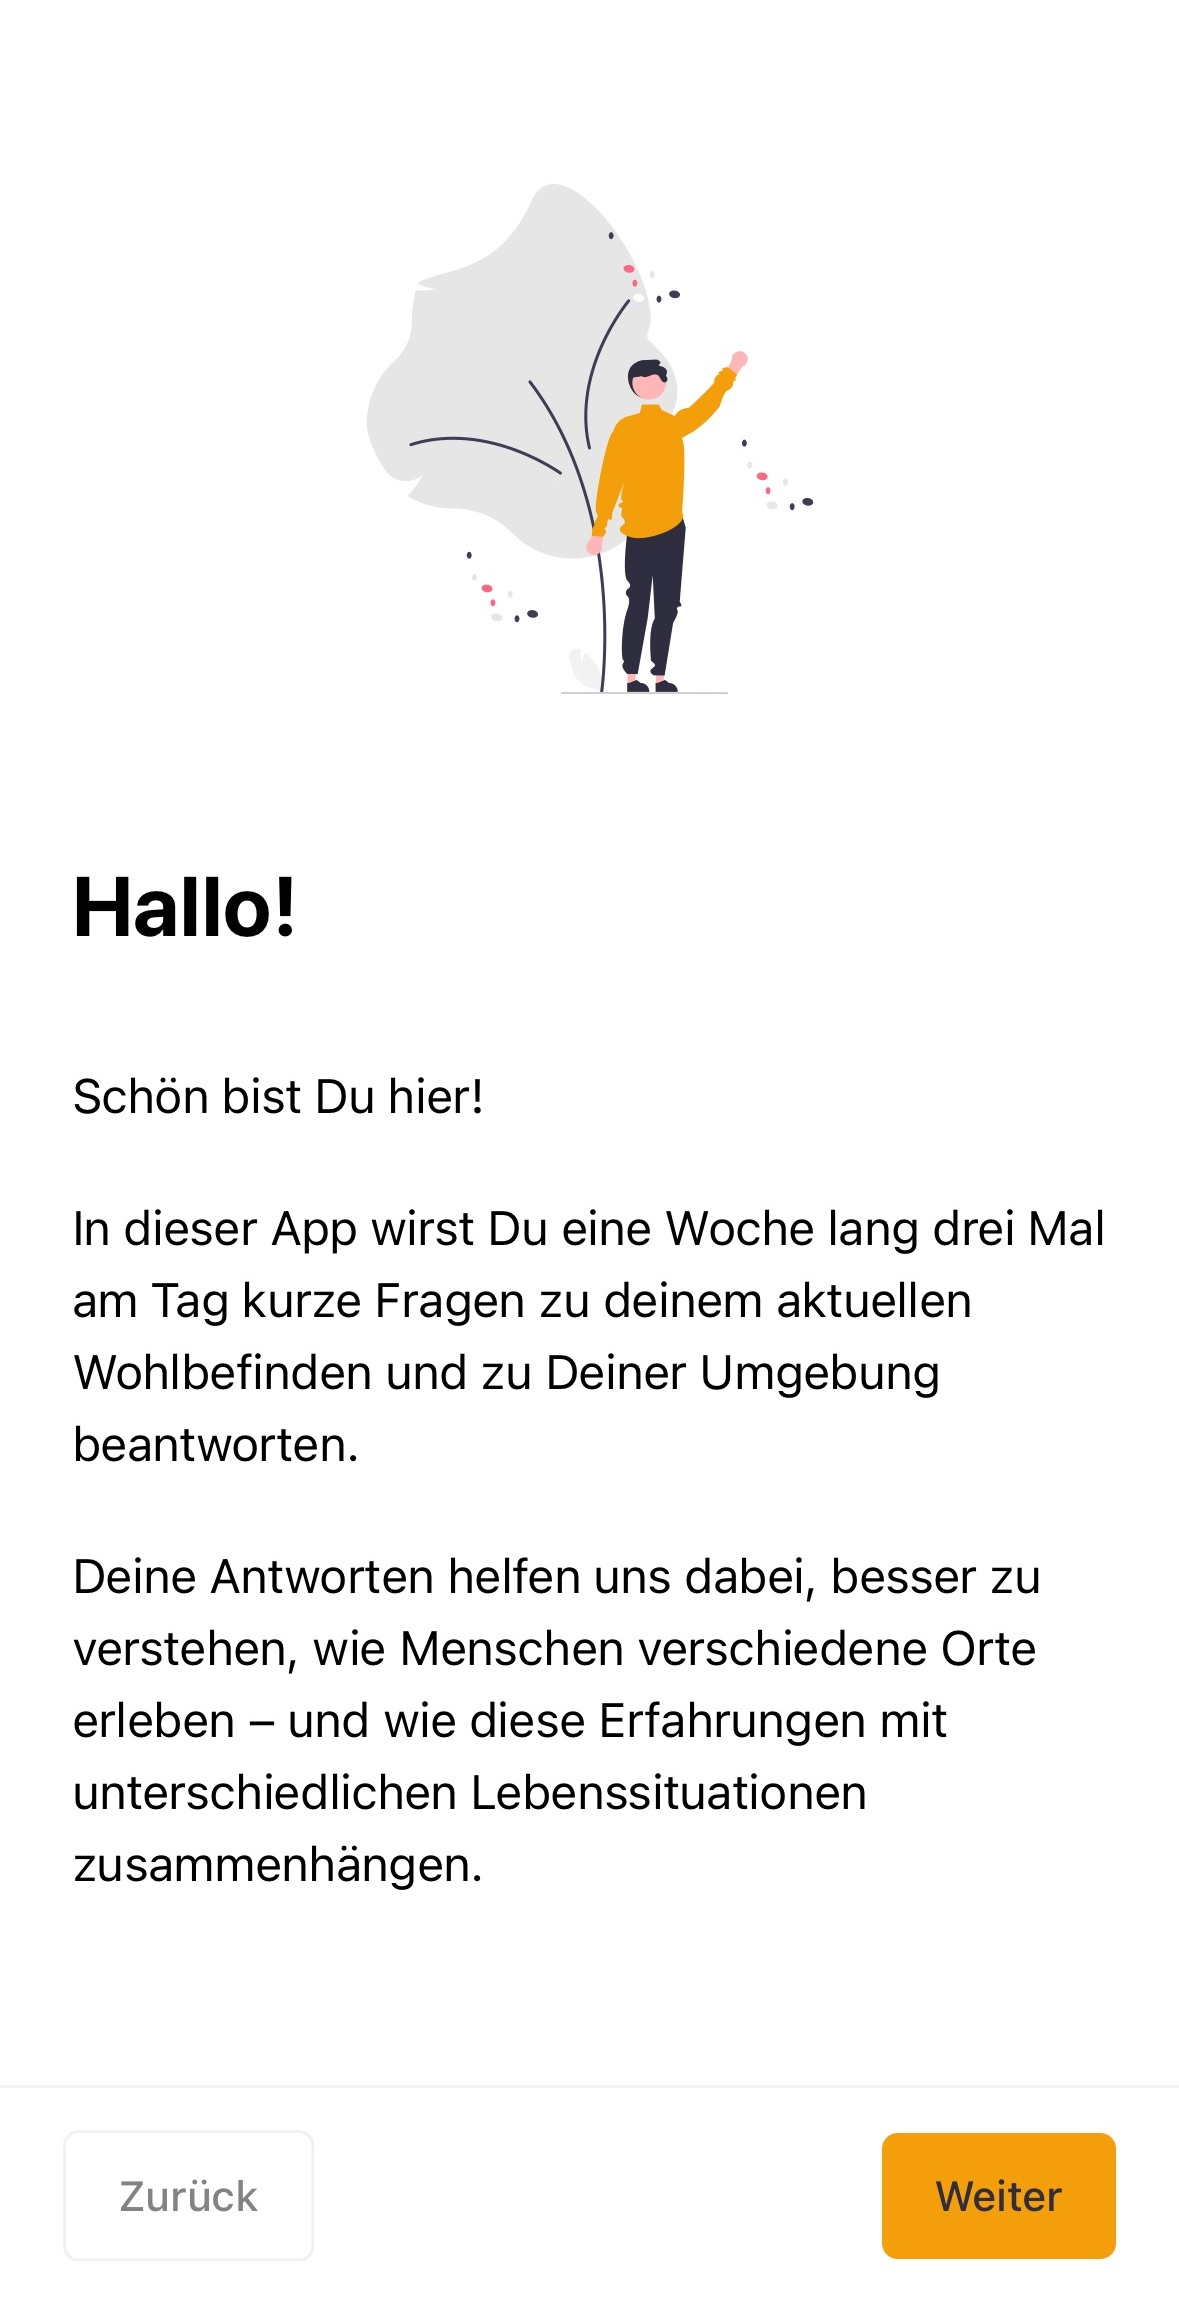
\includegraphics[width=\textwidth]{Arbeit/images/printscreens/welcome.jpeg}
        \caption{Begrüssungstext der App \textit{InterMind}}
        \label{fig:welcome}
    \end{minipage}
\end{figure}


Datenschutz spielte von Beginn an eine zentrale Rolle im Entwicklungsprozess und beeinflusste sowohl die technische Architektur als auch methodische Entscheidungen. Es wird konsequent dem Prinzip \textit{Privacy by Design} gefolgt, das vorsieht, Datenschutzanforderungen bereits bei der Konzeption einer Anwendung mitzudenken und nicht nachträglich zu ergänzen \parencite{cavoukianPrivacyDesign72009}. Ziel ist es, ein hohes Mass an Privatsphäre zu gewährleisten und gleichzeitig volle Transparenz über die Erhebung und Verarbeitung der Daten sicherzustellen.

In der Umsetzung wurde das Prinzip \textit{Privacy by Design} konkret durch technische Massnahmen wie \textit{privacy by architecture} realisiert \parencite{spiekermannEngineeringPrivacy2009}. Die App erfasst keine personenbezogenen Angaben wie Namen, Telefonnummern oder E-Mail-Adressen. Stattdessen wird beim ersten Start automatisch eine gerätegebundene \glsfirst{uuid} generiert, über die alle Daten pseudonymisiert zugeordnet werden. Eine kontinuierliche Ortung findet nicht statt; Standortdaten werden ausschliesslich zum Zeitpunkt einer beantworteten Befragung erhoben.


Die Speicherung der Daten erfolgt auf einem Server in der Schweiz unter Verwendung der Plattform \gls{supabase} und einer \gls{postgresql}-\gls{datenbank}. Eine Zugriffskontrolle auf Zeilenebene (\gls{rls}) stellt sicher, dass jedes Endgerät nur auf die eigenen Daten zugreifen kann. Alle Datenübertragungen zwischen App und Server sind verschlüsselt und erfolgen über authentifizierte Schnittstellen.

Teilnehmende können ihre Datensätze jederzeit direkt über die App löschen. Damit werden sämtliche Einträge, die mit ihrer \gls{uuid} verknüpft sind, dauerhaft entfernt. Die Kontrolle über die eigenen Daten bleibt somit vollständig bei den Nutzer\genderstern innen.

Alle datenschutzrelevanten Aspekte sind in einer eigenen Datenschutzrichtlinie dokumentiert, die über die App sowie auf der Projektwebseite\footnote{\href{https://intermind.ch/privacy-policy.html}{https://intermind.ch/privacy-policy.html}} öffentlich zugänglich ist. Die Richtlinie erläutert zudem die Rechte der Teilnehmenden nach Schweizer Datenschutzgesetz (\gls{dsg}) und der Europäischen Datenschutzgrundverordnung (\gls{dsgvo}).

\vspace{1em}

\begin{figure}[h]
    \centering
    \begin{minipage}[t]{0.38\textwidth}
        \centering
        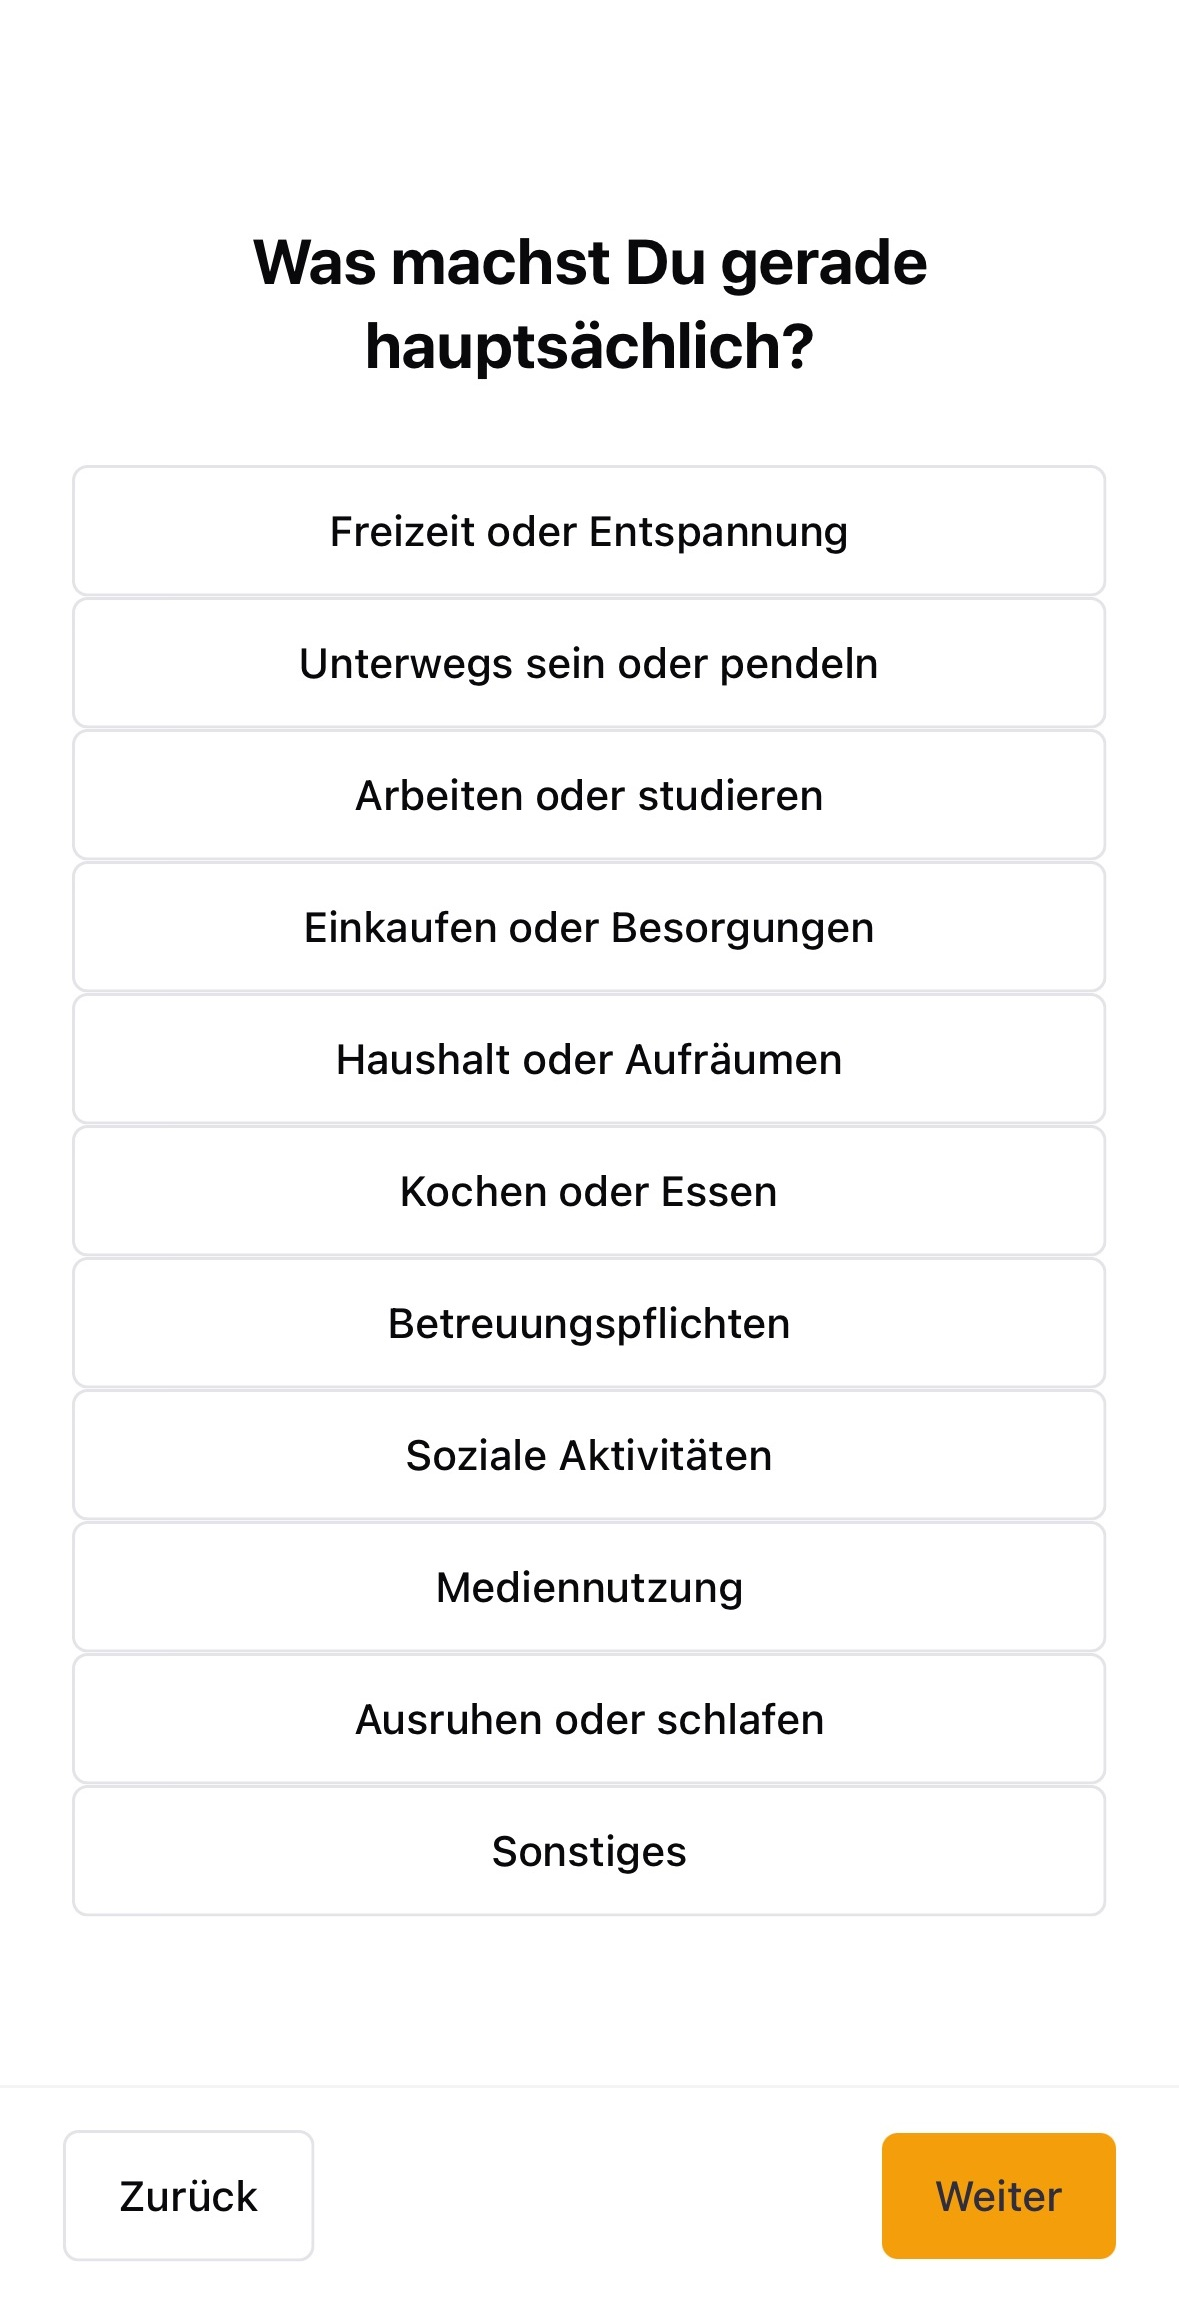
\includegraphics[width=\textwidth]{Arbeit/images/printscreens/beschaeftigung.jpeg}
        \caption{Multiple-Choice-Frage zur aktuellen Beschäftigung}
        \label{fig:beschaeftigung}
    \end{minipage}
    \hspace{0.1\textwidth}
    \begin{minipage}[t]{0.38\textwidth}
        \centering
        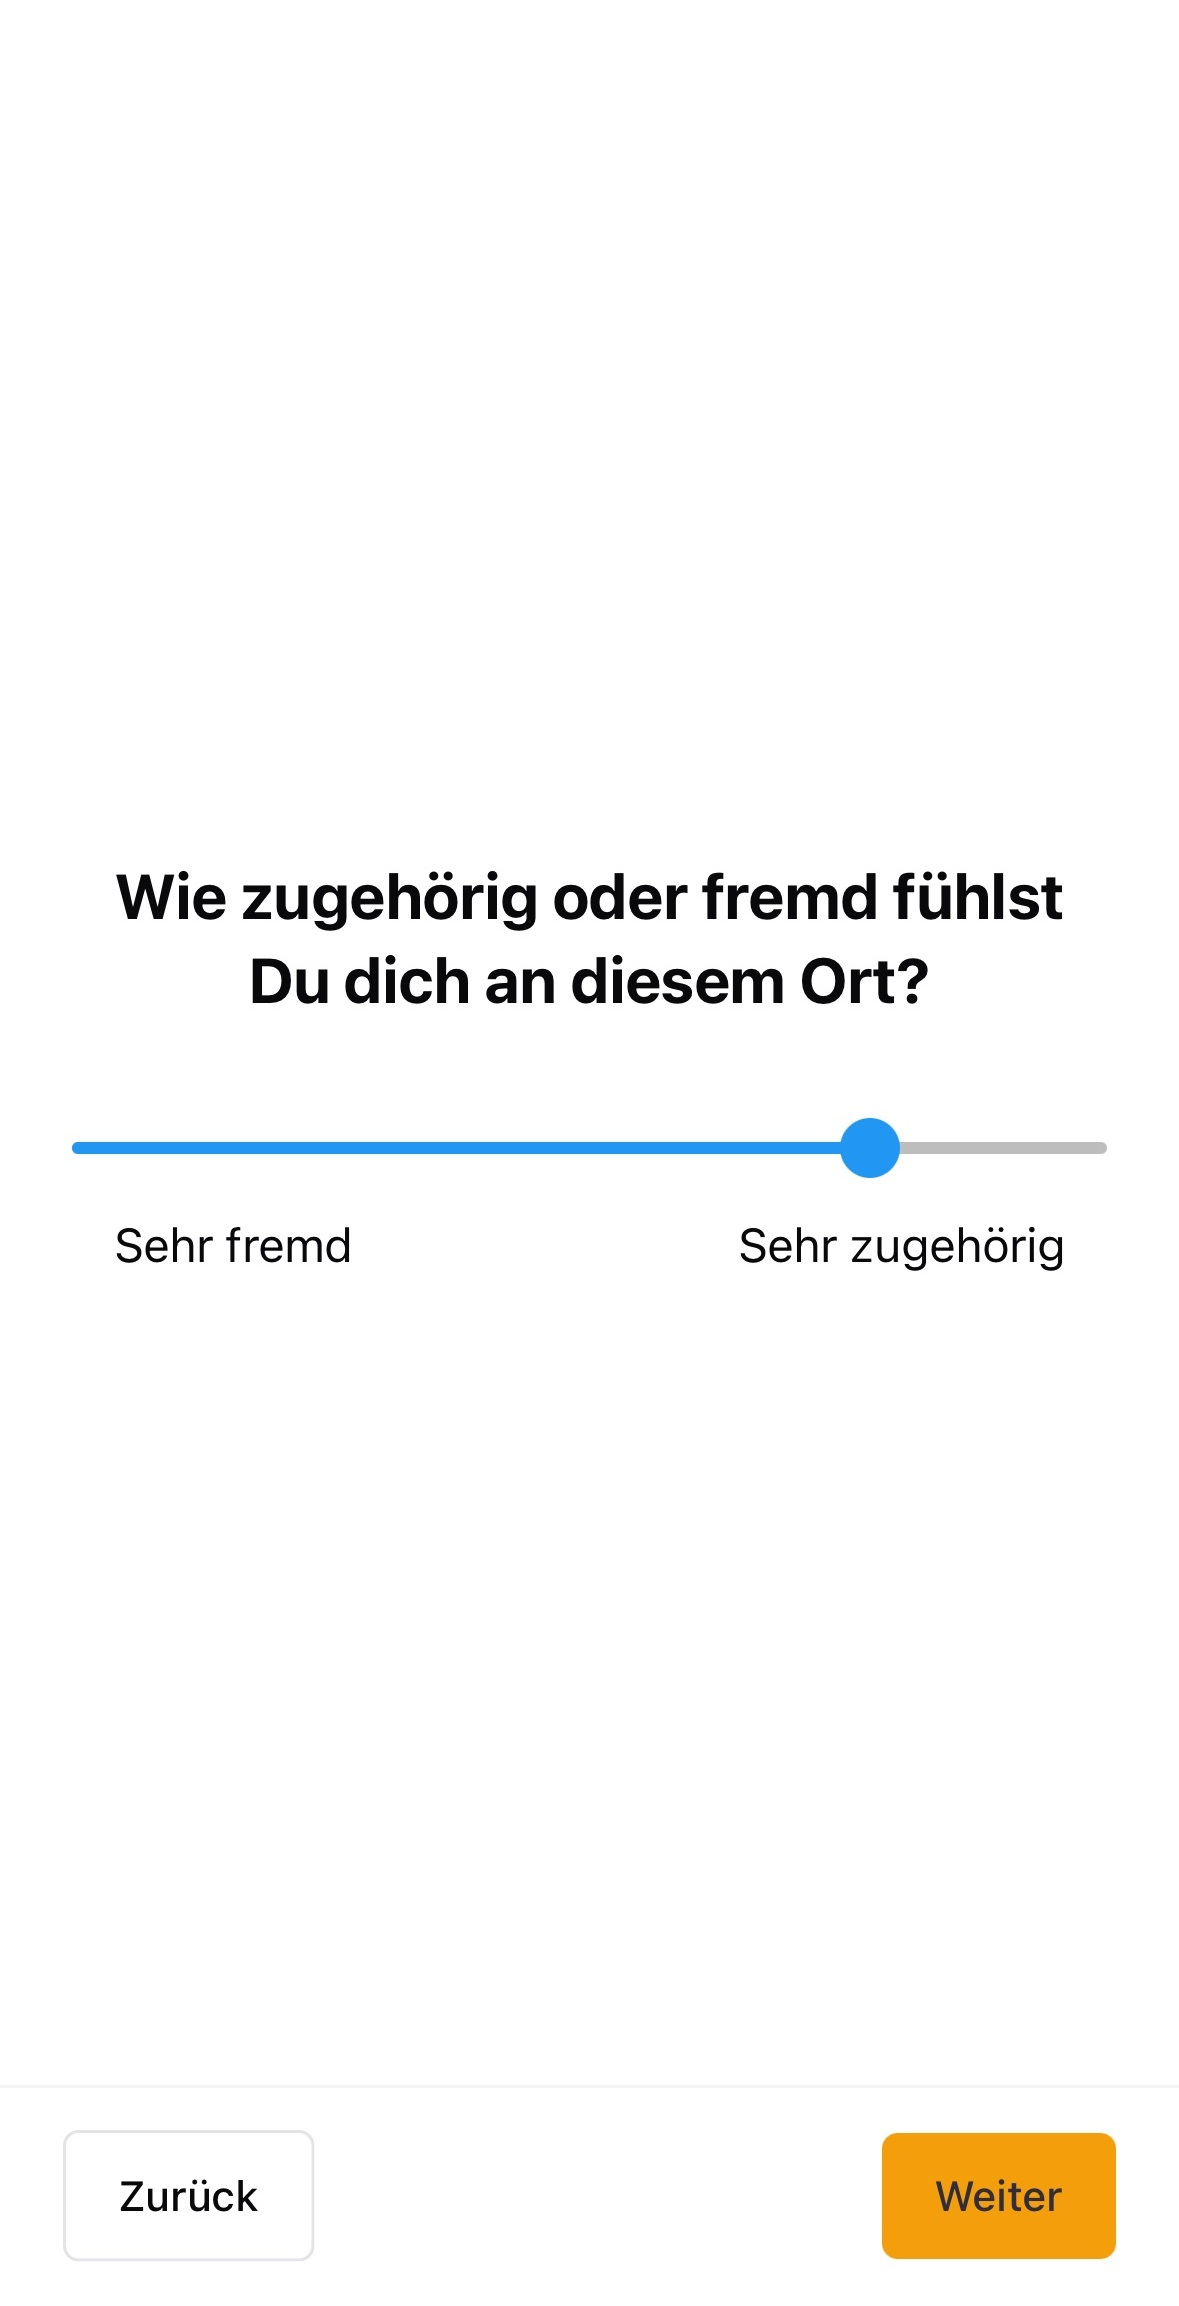
\includegraphics[width=\textwidth]{Arbeit/images/printscreens/zugehoerigkeit.jpeg}
        \caption{Slider-Frage zur sozialen Zugehörigkeit}
        \label{fig:zugehoerigkeit}
    \end{minipage}
\end{figure}


Die technische Umsetzung orientierte sich an etablierten Prinzipien des Software Engineerings \parencite{sommervilleSoftwareEngineering2016} sowie an den zentralen Gestaltungsprinzipien von \gls{solid} \parencite{martinCleanArchitectureCraftsmans2018}. Im Zentrum standen dabei eine saubere Trennung zwischen Anwendungslogik, Datenhaltung und Benutzeroberfläche, eine modulare Struktur der Komponenten sowie eine klare Zuordnung von Verantwortlichkeiten.

Für die Umsetzung wurde das \gls{framework} \gls{reactnative} in Kombination mit der Entwicklungsplattform \gls{expo} gewählt. Diese Entscheidung ermöglichte es, mit einer einheitlichen Codebasis sowohl \gls{ios}- als auch \gls{android}-Geräte zu unterstützen. Dadurch reduzierte sich der Entwicklungsaufwand, während gleichzeitig eine konsistente Benutzererfahrung auf beiden Plattformen sichergestellt werden konnte. Als serverseitige Infrastruktur kam \gls{supabase} zum Einsatz – ein \gls{opensource} \gls{backend}-as-a-Service auf Basis einer relationalen \gls{postgresql}-\gls{datenbank}, das \gls{authentifizierung}, \gls{autorisierung}, Datenspeicherung und sichere Datenübertragung integriert bereitstellt.

Der Fragenkatalog ist nicht im Quellcode verankert, sondern wird dynamisch über eine \gls{json}-Konfigurationsdatei aus der \gls{datenbank} geladen. Dadurch können Inhalte ohne App-Update angepasst werden, was weitestgehend verhindert, dass inkompatible Versionen der App entstehen. Diese Flexibilität erfordert jedoch eine aktive Internetverbindung für das Laden der Befragungsinhalte.

Nach dem erstmaligen Ausfüllen eines Fragebogens berechnet die App automatisch drei individuelle und zufällige Befragungszeitpunkte pro Tag. Diese werden lokal auf dem Gerät gespeichert. Die Zeitpunkte werden täglich zufällig innerhalb von drei Tagesabschnitten (Morgen, Mittag/Nachmittag, Abend) gewählt. Ein Mindestabstand zwischen den einzelnen Befragungen garantiert eine gleichmässige zeitliche Verteilung. Sobald ein Zeitpunkt erreicht ist, erhalten die Teilnehmenden eine Benachrichtigung und haben ab diesem Moment exakt eine Stunde Zeit, um den Fragebogen auszufüllen. Wird der Fragebogen nicht innerhalb dieser Zeitspanne ausgefüllt, verfällt der Slot und die App schickt eine weitere Benachrichtigung beim nächsten geplanten Zeitpunkt.

Das \gls{frontend} wurde minimalistisch und funktional gestaltet, um eine intuitive Nutzung zu ermöglichen und eine möglichst neutrale Darstellung der Fragen sicherzustellen \parencite{rogersInteractionDesignHumancomputer2023}. Die App gliedert sich in drei Hauptbereiche: einen Startbildschirm mit dem nächsten Befragungszeitfenster, den Fragebogenbereich und einen Informations- und Einstellungsbildschirm mit Hinweisen zum Datenschutz. Zur visuellen Unterstützung wurden generische \gls{opensource}-Vektorgrafiken von Katerina Limpitsouni\footnote{\href{https://undraw.co/}{undraw.co/}} verwendet.


\subsection{Von der Simulation zum Alltagstest – Feldtest und Feinschliff}
\label{sec:app_entwicklung_feldtest}

Zur Überprüfung der technischen Funktionsfähigkeit wurde ein zweistufiges Testverfahren durchgeführt, bestehend aus fortlaufenden Tests während der Entwicklung sowie einem abschliessenden internen Pretest. Auf automatisierte Tests wurde verzichtet, da deren Relevanz zu Beginn des Projekts unterschätzt wurde und eine nachträgliche Integration mit erheblichem Aufwand verbunden gewesen wäre. Stattdessen wurde ein manueller, iterativer Testansatz verfolgt. Die App wurde regelmässig mit \glspl{emulator} unterschiedlicher Bildschirmgrössen sowie auf physischen Geräten getestet. Die modulare Struktur der Codebasis sowie die Orientierung an den \gls{solid}-Prinzipien erleichterten dabei die gezielte Überprüfung einzelner Komponenten.

Im Zentrum der technischen Tests standen die dynamische Verarbeitung des Fragenkatalogs, die Datenübertragung an das \gls{supabase}-\gls{backend}, das Verhalten bei instabiler Internetverbindung sowie die lokale Planung von Push-Benachrichtigungen. Letztere erwiesen sich als besonders fehleranfällig, da die ursprüngliche Logik auf Hintergrundprozesse angewiesen war, die von beiden Betriebssystemen aus Effizienzgründen nicht immer zuverlässig gehandhabt werden.

Im Anschluss an die Implementierung wurde ein interner Pretest mit vier Personen durchgeführt. Die Testpersonen erhielten über die offiziellen Plattformen (\gls{testflight} und \gls{googleplayconsole}) Zugang zur App und nutzten diese über einen Zeitraum von zwei Wochen. Ziel war es, zentrale Funktionen unter Alltagsbedingungen zu überprüfen und Rückmeldungen zur allgemeinen Bedienbarkeit zu erhalten. Technische Aspekte wie das Verhalten beim ersten App-Start, die Stabilität der Datenerfassung und die Darstellung auf unterschiedlichen Geräten wurden dabei gezielt beobachtet.

Die Ergebnisse des Tests führten zu mehreren Anpassungen der App. So wurde bspw. die Logik zur Planung der Slots und Benachrichtigungen grundlegend überarbeitet: Anstelle von Hintergrundprozessen werden nun sämtliche Befragungszeitpunkte direkt nach dem Abschluss der ersten Befragung berechnet und lokal gespeichert. So konnten sämtliche Hintergrundprozesse eliminiert werden.

Zusätzlich wurden verschiedene kleinere Anpassungen an der Benutzeroberfläche vorgenommen, insbesondere im Hinblick auf die Darstellung von \gls{ui}-Elementen auf kleineren Bildschirmen sowie die Positionierung und Lesbarkeit von Slider-Beschriftungen. Diese Optimierungen trugen dazu bei, die visuelle Konsistenz der App auf verschiedenen Geräten zu verbessern.

\subsection{App-Veröffentlichung – Prozesse, Plattformen, Abhängigkeiten}

Um die entwickelte App für die eigentliche Datenerhebung nutzen zu können, wurde eine Veröffentlichung über die offiziellen App-Stores von Apple (iOS) und Google (Android) angestrebt. Beide Plattformen stellen dabei unterschiedliche technische, administrative und finanzielle Anforderungen, die den Veröffentlichungsprozess massgeblich beeinflussten.

Die Veröffentlichung im Apple App Store setzte zunächst den Erwerb einer kostenpflichtigen Entwicklerlizenz voraus, für die eine jährliche Gebühr von CHF 100 zu entrichten war. Nach erfolgreicher Einrichtung dieses Entwicklerkontos wurde die App zur Veröffentlichung eingereicht, allerdings von Apple zunächst nicht für eine finale Veröffentlichung im regulären App Store zugelassen. Als Begründung wurde angegeben, die App weise zu wenig inhaltlichen Mehrwert auf – eine Entscheidung, die aus Sicht der Entwicklung nur schwer nachvollziehbar war. Der Prüfprozess bei Apple ist zum Zeitpunkt des Abschlusses dieser Arbeit noch nicht vollständig abgeschlossen. Dennoch konnte die App über Apples eigene Plattform für öffentliche Beta-Tests (\gls{testflight}) bereitgestellt werden, sodass Teilnehmende der Studie über einen Link Zugang zur App erhielten.

Im Gegensatz dazu verlangte Google für eine Veröffentlichung im Android Play Store keine laufenden Lizenzkosten. Allerdings stellte Google die Bedingung, dass vor einer offenen Betaversion zunächst ein geschlossener Test mit mindestens 20 Personen über einen Zeitraum von zwei Wochen durchgeführt werden musste. Da es innerhalb des zeitlichen Rahmens dieser Bachelorarbeit nicht möglich war, eine ausreichende Anzahl Testpersonen mit Android-Geräten zu rekrutieren, wurde hierfür ein externer Dienstleister in Anspruch genommen, welcher diesen erforderlichen Test für eine Gebühr von CHF 30 durchführte. Nach erfolgreichem Abschluss dieses Tests wurde die App im Play Store als offene Beta veröffentlicht und war somit öffentlich verfügbar.

Darüber hinaus verlangten beide Plattformen, dass eine öffentlich zugängliche Datenschutzrichtlinie zur Verfügung steht. Zu diesem Zweck wurde eine Website\footnote{\href{https://intermind.ch/privacy-policy.html?lang=de}{intermind.ch/privacy-policy}} eingerichtet, auf der die vollständige Datenschutzerklärung einsehbar ist. Die Kosten hierfür beliefen sich auf einmalig CHF 10 für die Domainregistrierung; Hosting-Kosten entstanden keine zusätzlichen, da auf bereits bestehende Infrastruktur zurückgegriffen wurde.

\begin{figure}[h]
    \centering
    \begin{minipage}[t]{0.38\textwidth}
        \centering
        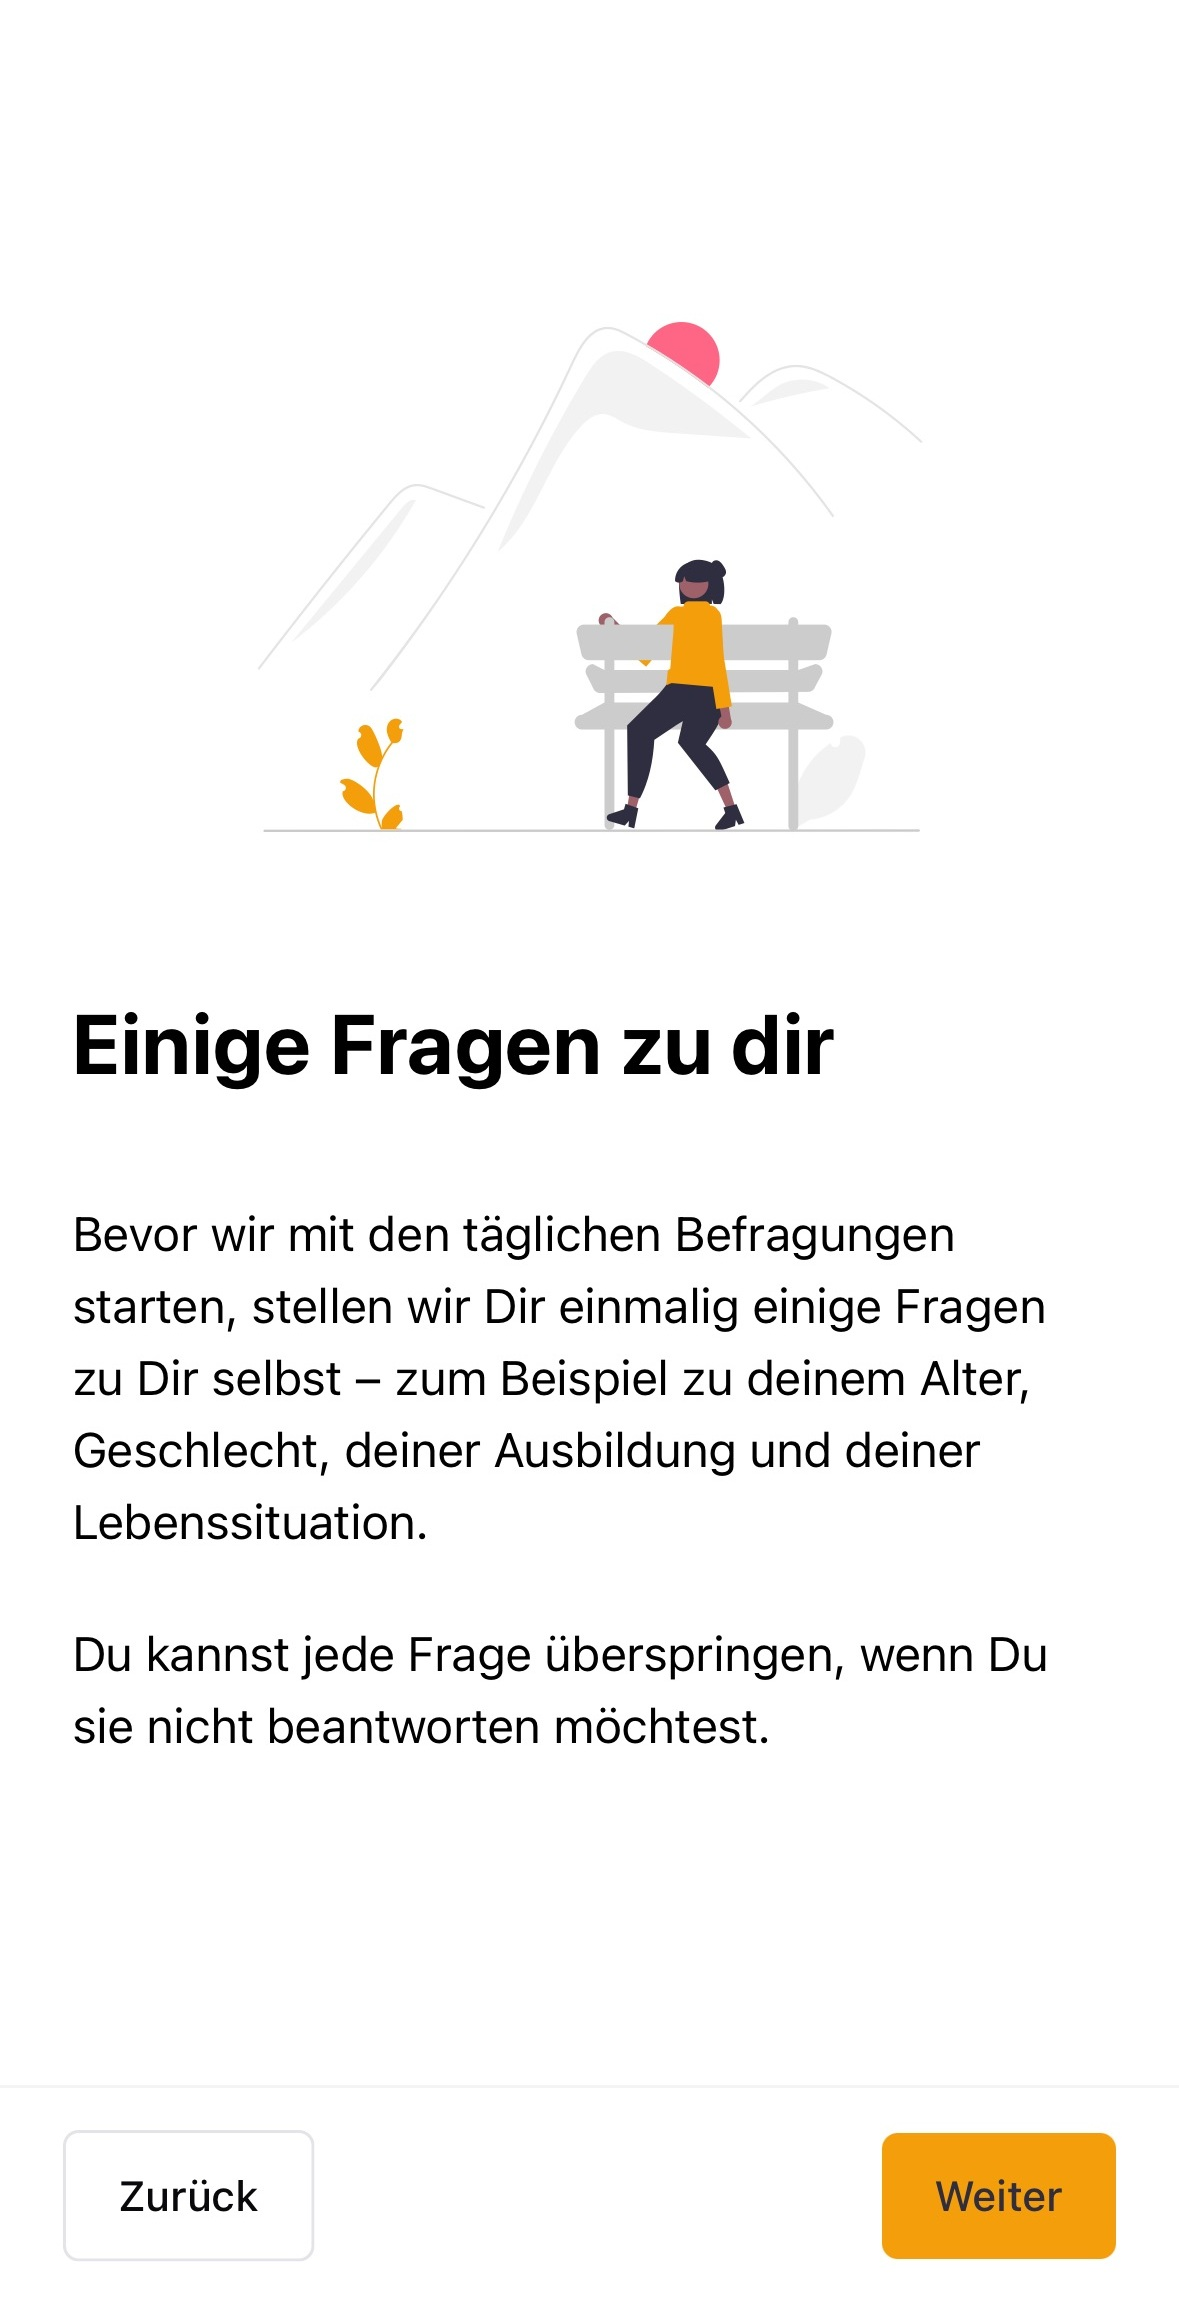
\includegraphics[width=\textwidth]{Arbeit/images/printscreens/fragen_zu_dir.jpeg}
        \caption{Überleitungsbildschirm zu den einmaligen Fragen}
        \label{fig:ueberleitungsbildschirm}
    \end{minipage}
    \hspace{0.1\textwidth}
    \begin{minipage}[t]{0.38\textwidth}
        \centering
        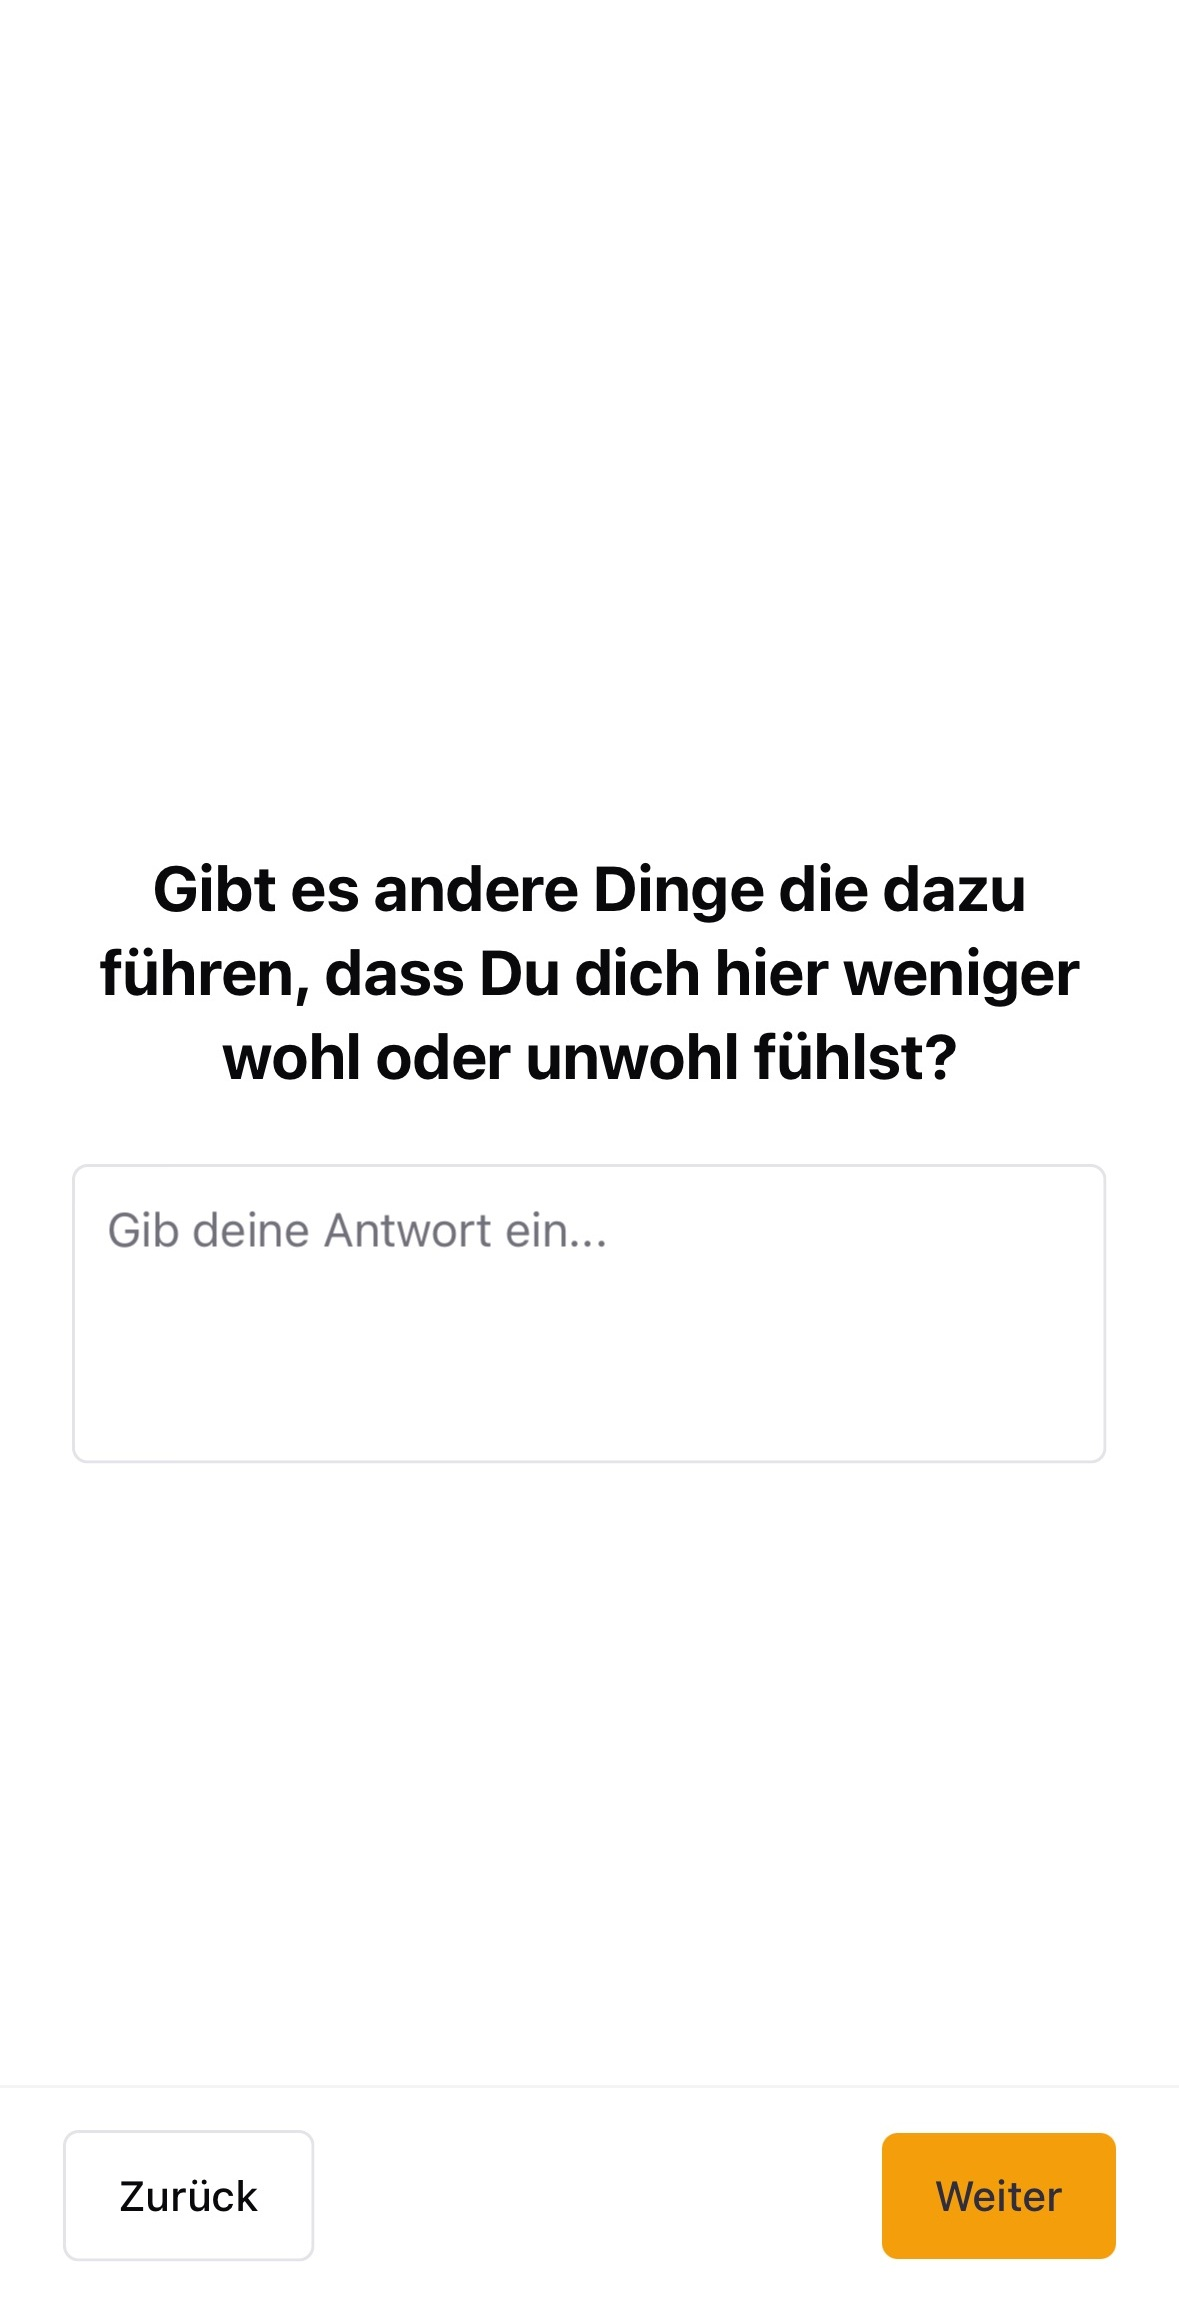
\includegraphics[width=\textwidth]{Arbeit/images/printscreens/offen_unwohl.jpeg}
        \caption{Offene Textfrage zu weiteren Gründen für Unwohlsein an diesem Ort}
        \label{fig:offene_textfrage}
    \end{minipage}
\end{figure}

\subsection{Eigenständig, aber nicht unabhängig – Entwicklung im Plattformzeitalter}

Die Entwicklung von \textit{InterMind} war mein erstes grösseres Projekt in \gls{typescript} und mit \gls{reactnative}. Die Umstellung vom strikt objektorientierten Denken in \gls{java} auf den dynamischeren, komponentenbasierten Ansatz war anspruchsvoll, aber enorm lehrreich. Insbesondere das konsequente Anwenden der \gls{solid}-Prinzipien half dabei, die Struktur der Anwendung nachvollziehbar zu halten – gerade in einem neuen Ökosystem. Die App funktioniert stabil, sieht gut aus, und hat ihren Zweck erfüllt.

Trotz einer bewussten Orientierung an Prinzipien wie \gls{solid} und einem grundlegenden Architekturkonzept zeigte sich im Verlauf der Entwicklung, dass eine noch systematischere Auseinandersetzung mit der Softwarearchitektur hilfreich gewesen wäre. Zwar wurde auf eine modulare Struktur geachtet, viele Designentscheidungen wurden jedoch eher situativ getroffen und nicht im Sinne eines übergeordneten Gesamtdesigns immer wieder überprüft. Gerade im weiteren Projektverlauf wäre es sinnvoll gewesen, gezielt zu früheren architektonischen Überlegungen zurückzukehren und diese zu reflektieren oder anzupassen.

Methoden wie \emph{Test-Driven Development} hätten diesen Prozess zusätzlich stützen können, indem sie klare Schnittstellen und Verantwortlichkeiten frühzeitig erzwingen. Auch der Aufbau automatisierter Tests und eine kontinuierlich integrierte Codeanalyse hätten dazu beigetragen, Fehlerquellen frühzeitig zu identifizieren und die langfristige Wartbarkeit der Anwendung zu verbessern. Viele kleinere Schwächen im Code wurden zwar pragmatisch behoben, ein strukturierteres Qualitätsmanagement hätte jedoch die Notwendigkeit späterer Refactoring-Prozesse deutlich reduziert.

In diesem Sinne reiht sich die App auch in eine typische Dynamik vieler \gls{opensource}-Projekte ein: Sie wurde aus einem konkreten Forschungsbedarf heraus entwickelt, funktioniert zuverlässig, ist öffentlich dokumentiert – aber nicht in jedem Teilbereich optimal strukturiert. Durch die Offenlegung des Quellcodes besteht jedoch die Möglichkeit, dass andere Entwickler\genderstern innen auf dieser Grundlage aufbauen, Verbesserungsvorschläge einbringen oder eigene Erweiterungen umsetzen.

Die Erfahrungen rund um die Veröffentlichung in den App Stores hat zentrale Spannungsfelder digitaler Infrastruktur deutlich gemacht. Obwohl die App funktional einsatzbereit war und über TestFlight bzw. den Play Store zugänglich gemacht werden konnte, blieb die reguläre Veröffentlichung im Apple App Store aufgrund einer intransparenten Ablehnung verwehrt.

Solche Prozesse offenbaren strukturelle Abhängigkeiten, die weit über dieses Projekt hinausgehen: Zwei gigantische multinationale Tech-Konzerne kontrollieren in weiten Teilen den Zugang zu digitaler Infrastruktur. Dabei wirken sie zugleich als Regelsetzer, Infrastrukturbetreiber und ökonomische Gatekeeper. Diese doppelte Rolle ist nicht demokratisch legitimiert, aber mit erheblicher Lenkungsmacht verbunden. Gerade nicht-kommerzielle, experimentelle oder aktivistische Projekte sind von diesen Kontrollmechanismen besonders betroffen, da sie sich nicht ohne Weiteres den geforderten Verwertungslogiken oder Standardprozessen unterwerfen.

Auch wenn Open-Source-Prinzipien allein diese strukturellen Hürden nicht auflösen können, war die Entscheidung zur Veröffentlichung des Quellcodes dennoch zentral: Sie schafft Transparenz, ermöglicht Weiterentwicklung und signalisiert ein bewusstes Gegenmodell zu proprietären, intransparenten Systemen. Gleichzeitig offenbart sich hier ein grundlegendes Spannungsfeld: Die offene, zugängliche und gemeinschaftsorientierte Logik von \gls{opensource}-Software steht in einem scharfen Kontrast zu den geschlossenen, marktkontrollierten Strukturen kommerzieller Distributionsplattformen. Wer eine App entwickeln und öffentlich zugänglich machen will, ist faktisch gezwungen, sich diesen Plattformen zu unterwerfen.

Die Arbeit an der App war dabei nicht nur funktional motiviert, sondern auch von der Erfahrung getragen, ein eigenes digitales Werkzeug gestalten zu können – mit all seinen Herausforderungen, aber auch mit dem unmittelbaren Lernerfolg und der Freude am konkreten Entstehungsprozess. Gerade vor dem Hintergrund einer zunehmend von privatwirtschaftlichen Plattformen dominierten digitalen Infrastruktur bleibt die Fähigkeit, eigene Werkzeuge zu entwickeln, ein wichtiger Akt technischer Aneignung.

\clearpage

\section{Fragebogenentwicklung}
\label{sec:fragebogen}

Die Entwicklung des Fragebogens erfolgte unter Berücksichtigung verschiedener Zielsetzungen, die im Folgenden präzisiert und begründet werden. Anschließend wird der Aufbau des Fragebogens im Detail erläutert.

\subsection{Zielsetzungen}
\label{subsec:zielsetzungen}

\begin{enumerate}[label=(Z\arabic*)]
    \item \textbf{Kürze und Wiederholbarkeit:} 
    Der Fragebogen sollte für die Teilnehmenden in \emph{möglichst kurzer Zeit} beantwortbar sein (circa drei bis fünf Minuten pro Erhebung). Diese Anforderung beruht auf Erfahrungen in der Umfrageforschung, wonach die Abbruchquote bei zunehmender Befragungsdauer stark steigt \parencite{dillman_internet_2014, bradburn_asking_2004}. Gleichzeitig ist eine \emph{regelmäßige Wiederholbarkeit} intendiert, um Längsschnittdaten (bzw.\ Mehrfachmessungen) zu erzeugen. Ein kurzer Fragenkatalog erhöht die Wahrscheinlichkeit, dass Teilnehmende an mehreren Zeitpunkten bereitwillig Auskunft geben \parencite{krosnick_question_2009}.

    \item \textbf{Erfassung intersektionaler Aspekte des Wohlbefindens:}
    Soziale Kategorien wie Geschlecht, Alter, soziale Lage, sexuelle Orientierung oder ethnische Zugehörigkeit interagieren bei der Entstehung von \emph{privilegierten} und \emph{diskriminierten} Positionen \parencite{crenshaw_mapping_1991, collins_black_2002}. Das Ziel ist, verschiedene Dimensionen dieser sozialen Kategorien \emph{gleichzeitig} – im Sinne einer \emph{intersektionalen} Perspektive – abzubilden und zu untersuchen, wie stark sie das subjektive Erleben im Alltag beeinflussen \parencite{rodo-de-zarate_developing_2014}. Werden diese Aspekte konsequent in die Abfrage integriert, lassen sich feiner aufgeschlüsselte Erkenntnisse zu sozial bedingten Disparitäten im Wohlbefinden gewinnen.

    \item \textbf{Echtzeit- bzw.\ kontextnahe Erhebung:}
    Statt einer einmaligen retrospektiven Befragung soll das \emph{Ecological Momentary Assessment} (EMA) genutzt werden, um das Erleben \emph{in Echtzeit} oder zumindest zeitnah zum Geschehen zu erfassen \parencite{shiffman_ecological_2008, stone_ecological_1994}. Auf diese Weise wird das Risiko verzerrter Erinnerungsleistungen (\emph{Recall Bias}) reduziert. Zudem ermöglicht das EMA-Design, den Einfluss situativer Faktoren unmittelbar zu erkennen, was für dynamische Prozesse – etwa Tageszeiten- oder Ortswechsel – von besonderer Bedeutung ist \parencite{bakolis_urban_2018}.

    \item \textbf{Integrierte Geolokalisierung:}
    Da das Wohlbefinden häufig von räumlichen Kontexten abhängt (z.\,B.\ privat vs.\ öffentlich, urban vs.\ ländlich), sollen Standortdaten (GPS) erhoben werden. Dieser Ansatz kann aufzeigen, in welchen Orten sich Diskriminierung, Sicherheit oder (Un-)Wohlbefinden verstärken bzw.\ abschwächen \parencite{rodo-de-zarate_developing_2014}. Die Verknüpfung von sozialer und räumlicher Dimension trägt somit zu einer umfassenderen Analyse bei, welche die räumliche Verteilung von Erfahrungen erfasst \parencite{bakolis_urban_2018}.

    \item \textbf{Wissenschaftliche Güte:}
    Das Instrument sollte hinsichtlich \emph{Validität}, \emph{Reliabilität} und \emph{Objektivität} hinreichend fundiert sein \parencite{dillman_internet_2014}. Hierzu ist vorgesehen, (a) etablierte Kurzskalen (etwa die Short-Version der Warwick-Edinburgh Mental Wellbeing Scale) zu adaptieren, (b) klar formulierte Items zu entwickeln, die sich in Pretests bewähren, und (c) standardisierte Formate zur Datenerhebung (z.\,B.\ einheitliche App-Interface) zu verwenden \parencite{tennant_warwick-edinburgh_2007, krosnick_question_2009}.

    \item \textbf{Minimierung der Teilnehmerbelastung:}
    Um hohe Rücklauf- und Verbleibquoten zu erzielen, wird auf unnötige Redundanz verzichtet. Daher werden z.\,B.\ demografische Basisdaten nur einmalig beim Erststart erhoben, während die kurzen Wohlbefindens- und Intersektionalitäts-Items in \emph{wiederholten} Befragungen fokussiert abgefragt werden. Dieses Vorgehen orientiert sich an Best Practices der EMA-Forschung, die belegen, dass eine zu hohe Itemanzahl pro Erhebung die Teilnahmebereitschaft mindern kann \parencite[vgl.]{shiffman_ecological_2008}.
\end{enumerate}

\noindent
Die genannten Ziele greifen komplementär ineinander: Die \emph{Kürze} und das \emph{wiederholte} Befragungsdesign (Ziel Z1) unterstützen die \emph{Echtzeit}-Perspektive (Z3) und erzeugen hochfrequente Daten, die sich mit dem \emph{intersektionalen} Anliegen (Z2) verknüpfen lassen. Darüber hinaus erlaubt die Einbeziehung von \emph{Geolokalisierung} (Z4) eine standortbezogene Analyse, sodass sowohl soziale als auch räumliche Strukturen sichtbar werden. Schließlich soll das Instrument hohe \emph{wissenschaftliche Güte} (Z5) vorweisen und die Belastung für Teilnehmende (Z6) so gering wie möglich halten.


\subsection{Theoretische und methodische Grundlage}
Im Kern basiert die Fragebogenkonzeption auf zwei Strängen der Forschung. Erstens wird das \emph{Ecological Momentary Assessment} (EMA) zugrunde gelegt, das bereits in verschiedenen Studien – etwa bei \parencite{shiffman_ecological_2008} oder \parencite{bakolis_urban_2018} – erfolgreich eingesetzt wurde, um subjektives Wohlbefinden und kontextuelle Faktoren in Alltagssituationen kontinuierlich zu erheben. EMA ermöglicht eine zeitnahe und kontextbezogene Messung, die sogenannte \emph{Recall Biases} reduziert und Veränderungen im Befinden in nahezu \emph{Echtzeit} abbildet \parencite{stone_ecological_1994}.

Zweitens wird die Konzeption von \emph{Intersektionalität} berücksichtigt, wie sie unter anderem bei \parencite{crenshaw_mapping_1991} und \parencite{collins_black_2002} ausgeführt wird. Die Annahme ist, dass soziale Kategorien (wie Geschlecht, Ethnizität, Klasse oder sexuelle Orientierung) nicht isoliert betrachtet werden können, sondern sich gegenseitig durchdringen. Im Kontext dieser Arbeit wird darauf Bezug genommen, indem die Teilnehmenden \emph{wiederholt} einschätzen, inwieweit unterschiedliche Kategorien ihr aktuelles Wohlbefinden begünstigen oder einschränken. Zur Visualisierung solcher mehrdimensionaler Daten bieten sich Methoden wie die \emph{Relief Maps} an, um variierende Erfahrungen mit Diskriminierung oder Privilegierung in Abhängigkeit vom Ort sichtbar zu machen \parencite{rodo-de-zarate_developing_2014}.

\subsection{Aufbau und Ablauf des Fragebogens}
Der Fragebogen ist in zwei Hauptteile gegliedert:

\begin{enumerate}[label=(\Alph*)]
  \item \textbf{Einmalige Erhebung von Basisdaten:}  
  Bei der ersten Teilnahme werden demografische und kontextuelle Informationen erfragt, die sich im Regelfall nicht kurzfristig ändern. Dazu zählen:
  \begin{itemize}
    \item Alter (als numerische Angabe).
    \item Geschlechtsidentität (bspw.\ weiblich, männlich, divers / trans / inter* sowie Freitextoption).
    \item Sexuelle Orientierung (beispielsweise hetero, schwul/lesbisch, bi/pan, asexuell, keine Angabe).
    \item Ethnische Zugehörigkeit oder Migrationshintergrund.
    \item Sozioökonomische Lage (etwa Ausbildungsstand, Beruf, Selbsteinschätzung bezüglich Klasse).
  \end{itemize}
  Diese Erfassung wird einmalig beim ersten App-Start durchgeführt, um redundante Abfragen in den späteren Kurzbefragungen zu vermeiden \parencite{dillman_internet_2014}. So bleibt der Zeitaufwand bei wiederholten Erhebungen minimal.

  \item \textbf{Wiederholte Kurzbefragung:}  
  Für die eigentliche EMA-Komponente erhalten die Teilnehmenden mehrmals täglich (beispielsweise zwei- bis viermal) eine kurze Push-Benachrichtigung. Pro Erhebung (Dauer: ca.\ 3--5 Minuten) werden die folgenden inhaltlichen Module durchlaufen:
  \begin{itemize}
    \item \emph{Standort und Situation}: Erfassung des Ortes via GPS (mit Einverständnis) und ggf.\ Auswahloptionen (z.\,B.\ ,,Zuhause'', ,,Draußen'', ,,am Arbeitsplatz'').
    \item \emph{Subjektives Wohlbefinden}: Abfrage über zwei bis drei Kurzskalen-Items, angelehnt an etablierte Instrumente wie die \emph{Short Warwick-Edinburgh Mental Wellbeing Scale (WEMWBS)} \parencite{tennant_warwick-edinburgh_2007} oder ähnliche Verfahren. 
    \item \emph{Intersektionale Aspekte}: Einschätzung, inwieweit Kategorien wie Geschlecht, Alter, soziale Lage, ethnische Zugehörigkeit oder sexuelle Orientierung im aktuellen Kontext das persönliche Wohlbefinden fördern bzw.\ behindern \parencite{collins_black_2002, crenshaw_mapping_1991}. 
    \item \emph{Freitext (optional)}: Möglichkeit, Besonderheiten oder subjektive Eindrücke der Situation zu ergänzen.
  \end{itemize}
\end{enumerate}

Dieser Aufbau zielt darauf ab, das \emph{Zeitbudget} der Teilnehmenden zu schonen und zugleich aussagekräftige Daten in \emph{mehrdimensionaler} Hinsicht zu gewinnen. Die Nutzung der ortsbezogenen Informationen erlaubt zudem eine raumbezogene Datenanalyse, um etwa Unterschiede zwischen öffentlichen und privaten Räumen zu untersuchen \parencite{bakolis_urban_2018, rodo-de-zarate_developing_2014}.

\subsection{Auswahl und Ausgestaltung der Items}
\subsubsection{Skalenlänge und Antwortformate}
Zur Messung psychologischer Konstrukte wie Wohlbefinden oder Stress wird häufig eine 5-Punkt-Likert-Skala verwendet \parencite{likert_technique_1932}. Studien zeigen jedoch, dass bei gerader Itemzahl (z.\,B.\ 4 oder 6 Antwortkategorien) die Tendenz zur mittleren Kategorie verringert wird \parencite{bradburn_asking_2004}. Eine \emph{gerade} Anzahl zwingt Teilnehmende eher zu einer leichten Richtungstendenz, während eine \emph{neutrale} Mittelkategorie (also ungerade, z.\,B.\ 5 oder 7 Stufen) als legitime Antwortoption durchaus sinnvoll sein kann \parencite{krosnick_question_2009}.

In der vorliegenden Arbeit wird eine \emph{5-stufige} Likert-Skala gewählt, da sie in vielen Fragebogenstudien als praktikabel gilt und eine \emph{neutrale} Antwort ermöglicht. Zahlreiche Studien zur Wohlbefindensmessung basieren auf diesem Format, wodurch eine Vergleichbarkeit vereinfacht wird \parencite{tennant_warwick-edinburgh_2007}. Um eine ausreichende Differenzierung zu erhalten, wird zusätzlich erwogen, bei den intersektionalen Items auf eine 6- oder 7-Punkt-Skala zu setzen. Die endgültige Entscheidung wird anhand eines Pretests getroffen (siehe Abschnitt \ref{sec:gütekriterien}).

\subsubsection{Wohlbefinden}
Für das \emph{Wohlbefinden} kommen zwei bis drei Items zum Einsatz, die jeweils unterschiedliche Facetten abdecken. Als Beispiel:
\begin{enumerate}[label=\emph{(WB\arabic*)}]
  \item \emph{Stimmung}: ,,Wie ist die eigene Stimmung \textbf{im Moment}?'' (Skala: 1 = sehr schlecht bis 5 = sehr gut)
  \item \emph{Sicherheit/Respekt}: ,,Ich fühle mich an diesem Ort sicher und respektiert.'' (Skala: 1 = stimme überhaupt nicht zu bis 5 = stimme voll zu)
  \item \emph{Allgemeines Befinden}: ,,In diesem Augenblick habe ich das Gefühl, dass meine Bedürfnisse geachtet werden.'' (1--5)
\end{enumerate}
Diese Items sind angelehnt an Formulierungen aus Kurzversionen der WEMWBS oder ähnlichen validierten Wohlbefindensskalen \parencite{tennant_warwick-edinburgh_2007}.

\subsubsection{Intersektionale Einschätzung}
Angelehnt an \parencite{crenshaw_mapping_1991} und \parencite{rodo-de-zarate_developing_2014} erfolgt eine kompakte Abfrage, in welcher Teilnehmende angeben, wie stark sie sich durch spezifische soziale Kategorien in der jeweiligen Situation unterstützt oder benachteiligt fühlen. Übliche Dimensionen (Geschlecht, soziale Lage, ethnische Zugehörigkeit, sexuelle Orientierung, Alter) können in Form einer Mini-Matrix abgefragt werden. Eine mögliche Formulierung lautet:

\begin{quote}
  \emph{,,In welcher Weise beeinflussen die folgenden Aspekte Ihr momentanes Befinden?''} \\
  \textbf{A:} Geschlechtsidentität \quad
  \textbf{B:} Alter \quad
  \textbf{C:} finanzielle / soziale Lage \quad
  \textbf{D:} Ethnische Herkunft \quad
  \textbf{E:} sexuelle Orientierung \\
  \textit{(Antwortskala 1--5: 1 = gar nicht eingeschränkt / eher unterstützt, 3 = neutral, 5 = stark eingeschränkt.)}
\end{quote}

So entsteht eine mehrdimensionale Einschätzung, die im nächsten Schritt visualisiert werden kann (z.\,B.\ mithilfe der \emph{Relief Maps} nach \cite{rodo-de-zarate_developing_2014}) oder durch statistische Analysen mit dem konkreten Ort (GPS-Koordinaten) verknüpft wird.

\subsection{Wissenschaftliche Gütekriterien und Pretest}
\label{sec:gütekriterien}
Die inhaltliche und formale Gestaltung des Fragebogens orientiert sich an etablierten Qualitätsanforderungen:
\begin{itemize}
    \item \textbf{Objektivität}: Die Items und Instruktionen werden in einer einheitlichen App-Oberfläche präsentiert. Die Daten werden automatisiert erfasst, wodurch Interviewerbias minimiert wird \parencite{dillman_internet_2014}.
    \item \textbf{Reliabilität}: Durch mehrfache \emph{repeated measures} und konsistente Skalen lässt sich eine gewisse Messpräzision erreichen. Unklare oder missverständliche Fragen werden vermieden, indem sie in einem Vorabtest identifiziert und überarbeitet werden \parencite{krosnick_question_2009}.
    \item \textbf{Validität}: Die Konstrukte (z.\,B.\ Wohlbefinden) sind in der Literatur verankert. Durch die Verknüpfung mit bewährten Verfahren (z.\,B.\ \emph{WEMWBS}) wird die Inhalts- und Konstruktvalidität gestärkt \parencite{tennant_warwick-edinburgh_2007}. Zudem gewährleistet das EMA-Design eine hohe \emph{ökologische Validität}, da Befragte ihre Angaben unmittelbar in Alltagssituationen machen \parencite{stone_ecological_1994}.
\end{itemize}

Zur finalen Absicherung der Items erfolgt ein \emph{Pretest} mit einer kleineren Gruppe von Probandinnen und Probanden (ca.\ 5--10 Personen), die den Fragebogen über mehrere Tage hinweg ausprobieren. Deren Rückmeldungen werden in Bezug auf Verständlichkeit, Länge und technische Handhabung ausgewertet. Anschließend werden eventuell zu komplexe oder mehrfach missverstandene Items angepasst \parencite{krosnick_question_2009}.

\subsection{Datenschutz und ethische Aspekte}
Alle Teilnehmenden erhalten zu Studienbeginn ausführliche Informationen über die freiwillige Teilnahme, das jederzeitige Widerrufsrecht und die sichere Datenspeicherung. Da \emph{Ortsdaten} (GPS) und potenziell sensible Angaben (etwa sexuelle Orientierung, ethnische Zugehörigkeit) abgefragt werden, wird besonderes Augenmerk auf die Umsetzung der \emph{Datenschutz-Grundverordnung (DSGVO)} gelegt \parencite{noauthor_verordnung_2016}. Sämtliche personenbezogenen Daten werden pseudonymisiert gespeichert und ausschließlich zu Forschungszwecken verwendet.

\subsection{Zusammenfassung und Ausblick}
Der hier entwickelte Fragebogen stellt ein auf \emph{Ecological Momentary Assessment} basierendes Instrument dar, um intersektionales Wohlbefinden an unterschiedlichen Orten und zu verschiedenen Zeitpunkten zu erfassen. Die gewählte Kombination aus kurzen, wiederkehrenden Skalen zur subjektiven Stimmung sowie einer Mini-Matrix für intersektionale Einflussfaktoren ermöglicht eine dynamische Perspektive auf das Erleben. Durch die Einbeziehung der Geolokalisierung lassen sich ortsabhängige Muster sichtbar machen. Zukünftig besteht die Möglichkeit, mithilfe der gesammelten Daten visuelle Auswertungen vorzunehmen (z.\,B.\ Heatmaps oder Relief Maps), die in der Tradition geografisch informierter Intersektionalitätsforschung stehen \parencite{rodo-de-zarate_developing_2014}.


\clearpage

\section{Pilotstudie}
\label{sec:pilotstudie}

\subsubsection{Ablauf und Durchführung der Datenerhebung}

Die Datenerhebung fand im Rahmen der einführenden Exkursion „Recht auf Stadt“ im ersten Studienjahr des Bachelorstudiengangs Geographie an der Universität Bern im Mai 2025 statt. Die teilnehmenden Studierenden wurden zu Beginn der Exkursion über Zielsetzung und Ablauf informiert und konnten anschliessend freiwillig an der Befragung teilnehmen. Die Nutzung der App wurde über den gesamten Exkursionszeitraum von drei Tagen durchgeführt, wobei die Teilnehmenden via Push-Benachrichtigungen mehrfach täglich aufgefordert wurden, die kurzen situativen Befragungen auszufüllen. Die Baseline-Befragung erfolgte einmalig zu Beginn.

Die Durchführung im Exkursionssetting ermöglichte eine kontrollierte Testung der technischen Funktionalität und eine hohe Compliance bei den Teilnehmenden. Gleichzeitig erlaubte dieses Setting, reale räumliche Kontexte, wie unterschiedliche urbane Umgebungen in Zürich, Basel und Bern, unmittelbar in die Datenerhebung einzubeziehen. Insgesamt zeichneten sich die Daten durch eine hohe räumliche und kontextuelle Varianz aus, die zentrale Grundlage für die späteren intersektionalen Analysen bildete.

Die vollständigen Fragebögen (Baseline- und situative Befragungen) sind als ergänzende Dokumentation digital im GitHub-Repository der App hinterlegt. Dies folgt dem Prinzip offener und transparenter Forschung. Eine detaillierte Fragebogenübersicht kann zusätzlich im Anhang dieser Arbeit eingesehen werden, um die inhaltliche Struktur und die Operationalisierung der theoretischen Konstrukte nachvollziehbar zu machen.

Zusammenfassend stellt die entwickelte App somit ein methodisch differenziertes, technisch flexibles Instrument dar, das sowohl situative Dynamiken als auch intersektionale soziale Strukturen systematisch erfassbar macht. Die enge Verknüpfung mit einem explizit intersektional ausgerichteten Fragebogen ermöglicht es, bestehende methodische Ansätze (Urban Mind, Relief Maps+) gezielt zu erweitern und dabei neue Erkenntnisse zur Beziehung von Raum, Wohlbefinden und sozialer Positionierung zu generieren.


\subsection{Limitationen und Herausforderungen der Datenerhebung}

\subsubsection{Geringe Rücklaufquote und mögliche Ursachen}

\subsubsection{Auswirkungen auf die Datenqualität und Analyse}

% LTeX: language=de-CH

\subsection{Ergebnisse} \label{sec:ergebnisse}

\subsubsection*{Beschreibung der Stichprobe}

Die Stichprobe des Probelaufs umfasst insgesamt 24 Personen. Die Mehrheit gehört der Altersgruppe \emph{16–25 Jahre} an (n = 20; 80\,\%). Nur wenige Personen entfallen auf die Gruppen \emph{26–35 Jahre} (n = 3; 12\,\%) und \emph{56–65 Jahre} (n = 1; 4\,\%); eine Person machte keine Altersangabe.

Bezüglich des \emph{sozialen Geschlechts} gaben 15 Personen (60\,\%) an, \emph{Mann} zu sein, 9 Personen (36\,\%) identifizierten sich als \emph{Frau}, und eine Person (4\,\%) als \emph{trans Mann}. Als biologisches Geschlecht gaben 16 Personen (64\,\%) an, \emph{männlich} zu sein, 8 (32\,\%) an, \emph{weiblich} zu sein, eine Person machte keine Angabe.

Die \cref{tab:kreuztabelle_abs} zeigt die Verteilung von sozialem Geschlecht und Altersgruppe (absolute Häufigkeiten).

\begin{table}[H]
    \centering
    \caption{Kreuztabelle: Soziales Geschlecht und Altersgruppe (absolute Häufigkeiten)}
    \label{tab:kreuztabelle_abs}
    \begin{tabular}{lccccc}
    \toprule
    \textbf{Geschlecht} & 16--25 & 26--35 & 56--65 & Keine Angabe & Gesamt \\
    \midrule
    Mann       & 12 & 2 & 0 & 1 & 15 \\
    Trans Mann &  0 & 0 & 1 & 0 & 1  \\
    Frau       &  8 & 1 & 0 & 0 & 9  \\
    \midrule
    \textbf{Gesamt} & 20 & 3 & 1 & 1 & 25 \\
    \bottomrule
    \end{tabular}
\end{table}

Weitere soziodemografische Merkmale der Teilnehmenden umfassen u.\,a. sexuelle Orientierung, Bildungsstand, Erwerbsstatus, Haushaltseinkommen, Haushaltsstruktur und -finanzierung, sowie Erfahrungen mit Diskriminierung. Eine vollständige Übersicht über die Verteilung dieser Merkmale findet sich in \cref{sec:appendix_demographics}.


Im Rahmen der Pilotstudie wurden insgesamt 106 Momentaufnahmen erhoben, verteilt auf die 25 Teilnehmenden. Die Anzahl abgeschlossener Befragungen pro Person variierte dabei erheblich (\textit{M} = 4{,}2; \textit{SD} = 2{,}9; \textit{Min} = 1; \textit{Max} = 12), was auf eine ungleichmässige Nutzung der App innerhalb der Teilnehmendengruppe hinweist (siehe \cref{fig:survey_counts}).

Die Tätigkeiten, die während der Beantwortung der Umfrage durchgeführt wurden, decken ein breites Spektrum ab. Am häufigsten gaben Teilnehmende an, zu arbeiten oder zu studieren (n = 48, 43\,\%), gefolgt von Freizeit- und Entspannungsaktivitäten (n = 19, 22\,\%) und Reisen bzw. Pendeln (n = 9, 10\,\%). Weitere Angaben umfassten etwa Kochen, Medienkonsum, soziale Aktivitäten oder Kombinationen mehrerer Aktivitäten.

Bezüglich des Aufenthaltsortes befanden sich die meisten Personen zum Zeitpunkt der Umfrage entweder an einer Bildungsinstitution (n = 38, 35\,\%) oder zu Hause (n = 28, 27\,\%). Weitere häufig genannte Orte waren unterwegs zu Fuss, per Fahrrad oder im Auto (n = 11, 11\,\%), öffentliche Verkehrsmittel (n = 8, 7\,\%) sowie die Wohnung anderer Personen oder Parks und Grünflächen (vgl. \cref{app:location_table}). Die Aufenthaltsorte verteilten sich dabei nahezu gleichmässig auf Innenräume (n = 54, 51\,\%) und Aussenräume (n = 52, 49\,\%).

Auch die soziale Situation während der Umfrage war sehr unterschiedlich: Ein Drittel der Momentaufnahmen wurde allein durchgeführt (n = 37, 35\,\%), ein weiteres Drittel in Gegenwart von Freund*innen (n = 28, 26\,\%). Weitere häufige Angaben betrafen die Anwesenheit von Fremden (n = 10, 9\,\%), Kolleg*innen (n = 8, 8\,\%) oder verschiedenen Kombinationen dieser Gruppen (vgl. \cref{app:people_table}).

Diese Vielfalt an Tätigkeiten, Kontexten und sozialen Situationen zeigt das Potenzial des Erhebungsinstruments, subjektives Wohlbefinden in unterschiedlichen Alltagssituationen ökologisch valide zu erfassen.



\begin{figure}[htbp]
    \centering
    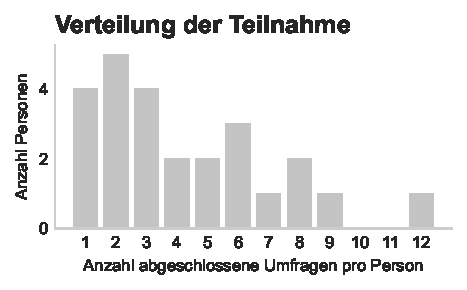
\includegraphics[width=8cm]{analysis/plots/survey_counts.pdf}
    \caption{Aufteilung nach Anzahl abgeschlossener Umfragen pro Person}
    \label{fig:survey_counts}
\end{figure}


\subsubsection*{Exemplarische Analysen mittels MAIHDA}
\label{sec:pilot_maihda}

In einem Probelauf wurde geprüft, ob die vorliegenden Daten eine intersektionale Multilevel-Analyse nach dem \gls{maihda}-Ansatz zulassen. Konkret sollte untersucht werden, ob (a) genügend Beobachtungen je intersektionalem Stratum vorhanden sind und (b) die zwischenstratale Varianz gross genug ist, um stabile Random-Effects-Schätzungen zu erhalten.

\paragraph{Iterative Spezifikation der Strata}
Ausgangspunkt war ein Set über alle erhobenen Achsen: Biologisches Geschlecht, Soziales Geschlecht, Sexuelle Orientierung, Ausbildungsstufe, Gruppiertes Äquivalenz-Einkommen, Anstellungsverhältnis, Geburtsland, Vorhandene Behinderungen.

Die Kombination dieser Merkmale ergab 20 unterschiedliche Strata. Die Zellgrössen (Anzahl Personen pro Stratum) sind allerdings sehr klein (siehe \cref{tab:zellgroessen_alle_achsen}).

\begin{table}[h]
    \centering
    \begin{tabular}{rl}
        count & 20 \\
        mean & 1.25 \\
        std & 0.55 \\
        min & 1 \\
        max & 3 \\
    \end{tabular}
    \caption{Zellgrössen pro Stratum mit allen Achsen}
    \label{tab:zellgroessen_alle_achsen}
\end{table}

Mit diesem Set von Strata ist die Modellierung nicht möglich, da die Zellgrössen zu klein sind und eine gute Schätzung der Varianzanteile nicht möglich ist.

Um die Modellierbarkeit zu erhöhen, wurde das Stratum anschliessend auf zwei theoretisch zentrale Achsen reduziert: Biologisches Geschlecht und Alter.

Dies führte zu insgesamt $6$ Strata, mit folgenden Zellgrössen:

\begin{table}[h]
    \centering
    \begin{tabular}{rl}
        count & 6 \\
        mean & 4.17 \\
        std & 4.7 \\
        min & 1 \\
        max & 12 \\
    \end{tabular}
    \caption{Zellgrössen pro Stratum mit reduzierten Achsen}
    \label{tab:zellgroessen_reduzierte_achsen}
\end{table}

Auch hier gibt es noch einzelne Strata mit weniger als 3 Beobachtungen.

\begin{table}[h]
    \centering
    \begin{tabular}{lll}
        Gender & Altersgruppe & Anzahl \\
        \hline
        man & 16 – 25 & 2 \\
        trans man & 56 – 65 & 1 \\
        man & missing & 1 \\
        woman & 26 – 35 & 1 \\
    \end{tabular}
    \caption{Strata mit weniger als 3 Beobachtungen}
    \label{tab:zellgroessen_reduzierte_achsen}
\end{table}

Trotzdem wurde versucht, mit diesem Set von Strata eine MAIHDA-Analyse durchzuführen.

Für jedes kontinuierliche Outcome (\texttt{sense\_of\_belonging}, \texttt{environmen\_pleasure}, \texttt{environment\_lively}, \texttt{environment\_nature}, \texttt{environment\_noise}) wurde ein zweistufiges MAIHDA-Setting geschätzt:
\begin{description}
    \item[Modell~1A (Nullmodell):] Zufallsinterzept auf Stratum-Ebene, keine festen Effekte der Achsen.
    \item[Modell~1B (Additives Modell):] Zusätzlich feste Haupteffekte von \texttt{age\_group} und \texttt{gender}; der verbleibende Stratum-Random-Effect wird als Interaktionsanteil interpretiert.
\end{description}
Aufgrund der geringen Zellgrössen wurde kein zusätzlicher Random-Intercept auf Personenebene modelliert. Die Schätzung erfolgte mittels \texttt{statsmodels.mixedlm} (MLE, Optimierer \texttt{lbfgs}).


Die geschätzten Varianzanteile zwischen Strata (Variance Partition Coefficient, VPC) waren durchgängig extrem klein. Beispielhaft:

\begin{center}
\begin{tabular}{lrrrr}
\toprule
Outcome & VPC$_{\text{Null}}$ & VPC$_{\text{add}}$ & PCV & $n$ (Zeilen) \\
\midrule
\texttt{sense\_of\_belonging}      & $1.24\times 10^{-5}$ & $1.15\times 10^{-6}$ & 90.7\% & 106 \\
\texttt{environmen\_pleasure}      & $\approx 0$          & $4.40\times 10^{-7}$ & --      & 106 \\
\texttt{environment\_lively}       & $2.95\times 10^{-4}$ & $3.43\times 10^{-5}$ & 88.2\%  & 106 \\
\texttt{environment\_nature}       & $1.03\times 10^{-2}$ & $1.12\times 10^{-6}$ & 99.99\% & 106 \\
\texttt{environment\_noise}        & $1.95\times 10^{-2}$ & $2.98\times 10^{-5}$ & 99.85\% & 106 \\
\bottomrule
\end{tabular}
\end{center}

Die nahezu Null liegenden VPCs belegen, dass (a) die Outcomes sich zwischen den Strata kaum unterscheiden und (b) die Stratum-Varianz im Modell auf Null \emph{geschrumpft} wird. PCV-Werte sind bei einem praktisch Null-VPC im Nullmodell numerisch instabil (z.\,B.\ negative oder extrem grosse Werte) und daher nicht interpretierbar.

\subsection{Schlussfolgerung}
Die Pilotanalyse zeigt, dass mit den vorliegenden Daten keine sinnvolle MAIHDA-Varianzzerlegung durchführbar ist. Gründe:
\begin{enumerate}
    \item \textbf{Zu kleine Strata-Zellgrössen}: Die meisten Strata enthalten nur eine Person bzw.\ sehr wenige Beobachtungen.
    \item \textbf{Geringe zwischenstratale Varianz}: Die betrachteten Outcomes variieren kaum zwischen den (reduzierten) Strata.
    \item \textbf{Numerische Instabilität}: Die Random-Effects-Kovarianzmatrix wird singular; die Schätzung kollabiert auf Randlösungen.
\end{enumerate}

\paragraph{Implikation für die weitere Analyse.}
Für die Beantwortung der Forschungsfrage (Einfluss situativer Umweltfaktoren auf affektives Wohlbefinden) bietet es sich an, die Umweltvariablen als Level-1-Prädiktoren in einem vereinfachten Modell (z.\,B.\ lineares Modell mit cluster-robusten Standardfehlern nach Person oder ein Mixed Model nur mit Personen-Random-Intercept) zu analysieren. Intersectionale Unterschiede können vorerst über feste Effekte (z.\,B.\ \texttt{C(age\_group)}, \texttt{C(gender)}) kontrolliert werden. Eine vollwertige MAIHDA-Anwendung ist erst mit grösserer Stichprobe und ausreichenden Zellgrössen pro Stratum sinnvoll.





\clearpage

% LTeX: language=de-CH

\chapter{Diskussion} \label{sec:diskussion}

\section{Potential und Grenzen des entwickelten Erhebungsinstruments}

Die Entwicklung von \textit{InterMind} war im Rahmen dieser Arbeit nicht nur ein technisches, sondern auch ein methodisches Experiment. Ziel war es, mit begrenzten Ressourcen ein Werkzeug zu schaffen, das situative, geolokalisierte Erhebungen zuverlässig durchführen kann -- und dabei die Grundprinzipien von Transparenz, Datenschutz und Anpassungsfähigkeit wahrt. Die im Kapitel skizzierten technischen Entscheidungen waren dabei stets auch methodische Abwägungen: Sie bestimmten nicht nur, wie die App funktioniert, sondern auch, welche Formen der Datenerhebung und -auswertung überhaupt möglich waren.

Besonders prägend war die Wahl eines bewusst reduzierten, clientseitig gesteuerten Systemdesigns. Diese Architektur minimierte Abhängigkeiten von externer Infrastruktur, reduzierte potenzielle Datenschutzrisiken und erlaubte eine transparente, vollständig nachvollziehbare Funktionsweise. Gleichzeitig bedeutete sie den Verzicht auf Funktionen, wie sie in komplexeren GEMA-Implementierungen üblich sind -- etwa geofence-basierte Trigger oder serverseitige Kontextlogiken. Dadurch blieb die App methodisch auf feste, vordefinierte Erhebungszeitpunkte beschränkt und konnte nicht adaptiv auf räumliche oder kontextuelle Veränderungen reagieren. Für explorative Pilotstudien wie die vorliegende war dies ausreichend, in längerfristigen oder gross angelegten Projekten wäre jedoch eine dynamischere, kontextsensitivere Architektur wünschenswert.

Die Entscheidung zur Open-Source-Veröffentlichung stellt einen zentralen Bestandteil des Projekts dar. Sie ermöglicht anderen Forschenden nicht nur die Nachnutzung des Codes, sondern schafft auch die Grundlage für kollaborative Weiterentwicklungen. Gleichzeitig machte die Erfahrung mit den App-Store-Gatekeeping-Prozessen deutlich, dass Offenheit allein keine Garantie für breite Zugänglichkeit ist: Die Distribution über zentrale Plattformen bleibt an kommerzielle und intransparente Strukturen gebunden, die auch nicht-kommerzielle, wissenschaftliche Projekte einschränken können. Hier zeigt sich ein strukturelles Spannungsfeld zwischen der offenen, gemeinschaftsorientierten Logik von Open-Source-Software und den geschlossenen, marktkontrollierten Ökosystemen der grossen Plattformanbieter.

Im Rückblick wird deutlich, dass die App-Entwicklung in dieser Form einerseits ein funktionierendes, forschungsnahes Werkzeug hervorgebracht hat, andererseits aber auch klare Grenzen aufweist. Diese liegen weniger in der Stabilität oder Bedienbarkeit, sondern vielmehr in der eingeschränkten Kontextanpassung, der fehlenden Echtzeitauswertung und der aufwändigen Anpassbarkeit für andere Forschungssettings. Zukünftige Iterationen könnten hier ansetzen -- etwa durch die Ergänzung serverseitiger Module, die Entwicklung eines webbasierten Dashboards für Monitoring und Feedback, oder die modularisierte Integration zusätzlicher Erhebungsmethoden.

Damit verdeutlicht \textit{InterMind} sowohl die Chancen als auch die Grenzen einer eigenständigen Entwicklung im Rahmen einer Abschlussarbeit: Sie eröffnet Handlungsspielräume, schafft technologische Unabhängigkeit im Entwicklungsprozess und macht Forschungsinfrastruktur transparent -- bleibt aber eingebettet in grössere, teils restriktive Strukturen, die den Handlungsspielraum letztlich mitbestimmen.

\section{Reflexion und Weiterentwicklungspotenzial des Fragebogens}

Der entwickelte Fragebogen erwies sich im Feld als grundsätzlich funktional und gut in den Ablauf der Studie integrierbar. Er erfüllte die Anforderung, situative Erhebungen in kurzer Zeit und mit geringer Belastung für die Teilnehmenden durchführen zu können. Gleichzeitig zeigte sich jedoch, dass diese Stärken teilweise mit methodischen Einbussen erkauft wurden, die den wissenschaftlichen Anspruch der Erhebung begrenzen.

Besonders deutlich wird dies bei der Auswahl der Items zur Erfassung situativen affektiven Wohlbefindens. Die gewählten Dimensionen -- darunter „generelles Wohlbefinden“, Zufriedenheit, Anspannung, Energie und Zugehörigkeit -- erlaubten zwar eine kompakte Erfassung, entstanden jedoch nicht aus einer stringenten theoretischen Modellierung heraus. Diese pragmatische Herangehensweise erleichterte zwar die Umsetzung im Rahmen einer Mehrfacherhebung, führte aber zu einer geringeren konzeptuellen Schärfe und erschwerte den direkten Vergleich mit bestehenden Studien.

Auch der Verzicht auf etablierte standardisierte Skalen hatte ambivalente Folgen. Er trug dazu bei, den Fragebogen schlank zu halten und die Akzeptanz bei den Teilnehmenden zu erhöhen, schränkte jedoch die Vergleichbarkeit der Daten und ihre Anschlussfähigkeit an bestehende Forschungsinstrumente ein. Eine gekürzte, modulare Integration validierter Skalen hätte hier einen Ausgleich zwischen Praktikabilität und methodischer Robustheit schaffen können.

Die mehrsprachige Umsetzung des Instruments war ein wichtiger Schritt in Richtung Zugänglichkeit, blieb jedoch ohne formalisierte Validierung durch muttersprachliche Expert:innen. Dadurch ist nicht auszuschliessen, dass inhaltliche Nuancen, insbesondere bei affektiven Zustandsbeschreibungen, zwischen den Sprachversionen leicht variierten. Diese Unsicherheiten verstärkten sich bei sensiblen Konzepten wie \gls[noindex]{race}, für das im deutschsprachigen Kontext keine etablierten, diskriminierungssensiblen Kategorien verfügbar sind. Die gewählte Operationalisierung über Geburts- und Aufenthaltsland senkte zwar die Erhebungsbarrieren, konnte die Komplexität rassifizierter Erfahrungen jedoch nur unvollständig erfassen.

Schliesslich war der Entwicklungsprozess des Fragebogens zwar iterativ angelegt und von kontinuierlichem Feedback begleitet, basierte jedoch nicht auf einem formalen Pretest mit einer breiten und divers zusammengesetzten Testgruppe. Dadurch wurden potenzielle Verständnisschwierigkeiten oder kulturelle Unschärfen nur in begrenztem Umfang sichtbar.

Insgesamt bleibt festzuhalten, dass der Fragebogen in seiner vorliegenden Form eine praktikable, aber methodisch eingeschränkte Lösung darstellt. Für zukünftige Studien bieten sich mehrere Ansatzpunkte zur Weiterentwicklung: eine engere theoretische Anbindung der Items, die gezielte Integration gekürzter validierter Skalen, ein systematischeres Übersetzungs- und Validierungsverfahren sowie umfassendere Pretests. Auf diese Weise liesse sich die inhaltliche Aussagekraft der Erhebung stärken, ohne die für hochfrequente Befragungen notwendige Niedrigschwelligkeit aufzugeben.

\section{Empfehlungen für weiterführende Forschung}

\subsection{Verbesserungsvorschläge zur Erhöhung der Teilnahmequote}

\subsection{Optimierung der intersektionalen Datenerhebung und Analyse}

\subsection{Integration qualitativer Verfahren}

% Standorterhebung nicht verwendet


% ohne technische details mal hier rüberkopiert:

% \section{Eigenständig, aber nicht unabhängig -- Entwicklung im Plattformzeitalter}

% Die Entwicklung von \gls{intermind} war mein erstes grösseres Projekt in \gls{typescript} und mit \gls{reactnative}. Die Umstellung vom strikt objektorientierten Denken in \gls{java} auf den dynamischeren, komponentenbasierten Ansatz war anspruchsvoll, aber enorm lehrreich. Insbesondere das konsequente Anwenden der \gls{solid}-Prinzipien half dabei, die Struktur der Anwendung nachvollziehbar zu halten -- gerade in einem neuen Ökosystem. Die App funktioniert stabil, sieht gut aus, und hat ihren Zweck erfüllt.

% Trotz einer bewussten Orientierung an Prinzipien wie \gls{solid} und einem grundlegenden Architekturkonzept zeigte sich im Verlauf der Entwicklung, dass eine noch systematischere Auseinandersetzung mit der Softwarearchitektur hilfreich gewesen wäre. Zwar wurde auf eine modulare Struktur geachtet, viele Designentscheidungen wurden jedoch eher situativ getroffen und nicht im Sinne eines übergeordneten Gesamtdesigns immer wieder überprüft. Gerade im weiteren Projektverlauf wäre es sinnvoll gewesen, gezielt zu früheren architektonischen Überlegungen zurückzukehren und diese zu reflektieren oder anzupassen.

% Methoden wie \emph{Test-Driven Development} hätten diesen Prozess zusätzlich stützen können, indem sie klare Schnittstellen und Verantwortlichkeiten frühzeitig erzwingen. Auch der Aufbau automatisierter Tests und eine kontinuierlich integrierte Codeanalyse hätten dazu beigetragen, Fehlerquellen frühzeitig zu identifizieren und die langfristige Wartbarkeit der Anwendung zu verbessern. Viele kleinere Schwächen im Code wurden zwar pragmatisch behoben, ein strukturierteres Qualitätsmanagement hätte jedoch die Notwendigkeit späterer Refactoring-Prozesse deutlich reduziert.

% In diesem Sinne reiht sich die App auch in eine typische Dynamik vieler \gls{opensource}-Projekte ein: Sie wurde aus einem konkreten Forschungsbedarf heraus entwickelt, funktioniert zuverlässig, ist öffentlich dokumentiert -- aber nicht in jedem Teilbereich optimal strukturiert. Durch die Offenlegung des Quellcodes besteht jedoch die Möglichkeit, dass andere Entwickler\genderstern innen auf dieser Grundlage aufbauen, Verbesserungsvorschläge einbringen oder eigene Erweiterungen umsetzen.

% \vspace{1em}

% Trotz stabiler Funktionalität und durchdachter Grundstruktur weist das entwickelte System klare Begrenzungen auf -- insbesondere im Hinblick auf die situative Reaktionsfähigkeit und Kontextanpassung. So verzichtet \gls{intermind} bewusst auf kontinuierliches Geotracking, automatisierte Trigger oder serverseitige Kontextlogiken, wie sie in anderen \acrshort{gema}-Systemen Anwendung finden.

% Ein Beispiel dafür bietet das im Rahmen einer kanadischen Studie zu Nationalparks entwickelte \acrshort{health}-Plattform \parencite{wrayHealthyEnvironmentsActive2025}. Die Dokumentation zu diesem Tool ist erst während der Entstehung dieser Arbeit als Preprint veröffentlicht worden. Die App wird derzeit exklusiv im Rahmen des \textit{ParkSeek}-Projekts\footnote{\href{https://parkseek.ca/}{parkseek.ca}} eingesetzt und ist nicht öffentlich zugänglich. Ihre zugrundeliegende Systemarchitektur erlaubt eine kontinuierliche Standorterfassung und serverseitige Kontextverarbeitung, wodurch komplexe Logiken wie geofence-basierte Trigger umgesetzt werden können. So lassen sich etwa Benachrichtigungen auslösen, wenn sich Teilnehmende über längere Zeit in spezifischen Umwelten aufhalten. Diese technisch anspruchsvolle Lösung erlaubt eine besonders enge Verzahnung zwischen räumlichem Verhalten und situativer Befragung, geht jedoch mit einem hohen Aufwand sowie erheblichen Anforderungen an Datenschutz, Datenmanagement und Infrastruktur einher.

% Im Rahmen eines Bachelorprojekts wäre die Implementierung eines derart umfassenden Systems weder zeitlich noch organisatorisch realistisch gewesen. Stattdessen wurde ein datensparsamer, clientseitig gesteuerter Ansatz gewählt, der mit begrenzten Mitteln eine funktionale, transparente und reflektierte Umsetzung ermöglicht. Die Entscheidung für ein reduziertes Systemdesign war damit nicht nur eine Frage des Aufwands, sondern auch ein bewusster Kompromiss zugunsten von Kontrollierbarkeit und Datenschutz.

% Eine weitere Limitation des aktuellen Systemdesigns liegt im Fehlen eines serverseitigen Dashboards oder einer integrierten Auswertungsoberfläche. Es besteht keine Möglichkeit, Rückmeldungen in Echtzeit zu visualisieren, aggregierte Antworten einzusehen oder Monitoring-Funktionen während der Erhebung zu nutzen. Solche Features wären insbesondere für die Steuerung längerer Erhebungsphasen, die Qualitätssicherung oder für Feedbackschleifen mit den Teilnehmenden von Vorteil gewesen. Ihre Umsetzung hätte jedoch zusätzliche Entwicklungsressourcen sowie eine komplexere Backend-Architektur vorausgesetzt. Gleichwohl bleibt die Möglichkeit bestehen, entsprechende Funktionen in zukünftigen Iterationen oder auf Basis der veröffentlichten Codebasis nachzurüsten.

% \vspace{1em}

% Die Erfahrungen rund um die Veröffentlichung in den App Stores hat zentrale Spannungsfelder digitaler Infrastruktur deutlich gemacht. Obwohl die App funktional einsatzbereit war und über TestFlight bzw. den Play Store zugänglich gemacht werden konnte, blieb die reguläre Veröffentlichung im Apple App Store aufgrund einer intransparenten Ablehnung verwehrt.

% Solche Prozesse offenbaren strukturelle Abhängigkeiten, die weit über dieses Projekt hinausgehen: Zwei gigantische multinationale Tech-Konzerne kontrollieren in weiten Teilen den Zugang zu digitaler Infrastruktur. Dabei wirken sie zugleich als Regelsetzer, Infrastrukturbetreiber und ökonomische Gatekeeper. Diese doppelte Rolle ist nicht demokratisch legitimiert, aber mit erheblicher Lenkungsmacht verbunden. Gerade nicht-kommerzielle, experimentelle oder aktivistische Projekte sind von diesen Kontrollmechanismen besonders betroffen, da sie sich nicht ohne Weiteres den geforderten Verwertungslogiken oder Standardprozessen unterwerfen.

% Auch wenn Open-Source-Prinzipien allein diese strukturellen Hürden nicht auflösen können, war die Entscheidung zur Veröffentlichung des Quellcodes dennoch zentral: Sie schafft Transparenz, ermöglicht Weiterentwicklung und signalisiert ein bewusstes Gegenmodell zu proprietären, intransparenten Systemen. Gleichzeitig offenbart sich hier ein grundlegendes Spannungsfeld: Die offene, zugängliche und gemeinschaftsorientierte Logik von \gls{opensource}-Software steht in einem scharfen Kontrast zu den geschlossenen, marktkontrollierten Strukturen kommerzieller Distributionsplattformen. Wer eine App entwickeln und öffentlich zugänglich machen will, ist faktisch gezwungen, sich diesen Plattformen zu unterwerfen.

% Die Arbeit an der App war dabei nicht nur funktional motiviert, sondern auch von der Erfahrung getragen, ein eigenes digitales Werkzeug gestalten zu können -- mit all seinen Herausforderungen, aber auch mit dem unmittelbaren Lernerfolg und der Freude am konkreten Entstehungsprozess. Gerade vor dem Hintergrund einer zunehmend von privatwirtschaftlichen Plattformen dominierten digitalen Infrastruktur bleibt die Fähigkeit, eigene Werkzeuge zu entwickeln, ein wichtiger Akt technischer Aneignung.

% auch hier nicht nochmal entwickelnd erklären, je nachdem acuh ganz sein lassen

% \section{Klar, verständlich, iterativ -- Der Weg zum finalen Fragebogen}

% Die sprachliche Gestaltung der Fragebogen-Items stellte im Entwicklungsprozess eine zentrale methodische Herausforderung dar. Ziel war es, die Befragung möglichst zugänglich, verständlich und gleichzeitig inhaltlich präzise zu gestalten. Da die Befragung explizit auf eine intersektionale Analyse abzielt, wurde besonderer Wert darauf gelegt, die sprachliche Zugänglichkeit möglichst breit zu gewährleisten. Folglich wurde der Fragebogen bewusst mehrsprachig konzipiert und auf Deutsch, Englisch sowie Französisch umgesetzt. Weitere Sprachversionen wären zwar aus Sicht der intersektionalen Zugänglichkeit wünschenswert gewesen, scheiterten jedoch am hohen Aufwand für qualitativ hochwertige und inhaltlich konsistente Übersetzungen.

% Ein grundsätzliches Anliegen war eine möglichst direkte, adressierende Sprache in der \enquote{Du}-Form, um einen niederschwelligen Zugang zur Befragung zu fördern und hierarchische Distanz zwischen Forschenden und Teilnehmenden zu reduzieren. Gleichzeitig mussten die Formulierungen prägnant, alltagsnah und schnell erfassbar sein, da insbesondere die situativen Erhebungen kurz gehalten werden sollten. Hier ergab sich ein methodischer Balanceakt: Einerseits sollte die Befragung leicht verständlich bleiben, andererseits mussten komplexe Konzepte in zugänglicher Sprache operationalisiert werden. So wurde \gls{bspw} das Konzept der \gls{intersektionalitaet} im Einführungsteil des Fragebogens erläutert, danach jedoch bewusst vermieden, um unnötige Barrieren zu reduzieren. Stattdessen wurden alternative Formulierungen wie \enquote{persönliche Merkmale} verwendet, die jedoch teilweise inhaltliche Unschärfen mit sich brachten. 

% Besonders deutlich wurde diese Herausforderung im Umgang mit dem Konzept \gls[noindex]{race}. Gerade im deutschsprachigen Kontext existieren hier nur schwer geeignete Begrifflichkeiten: Formulierungen wie \enquote{Rasse} oder \enquote{Ethnizität} sind entweder sprachlich ungebräuchlich, problematisch oder stark mit kolonialen und biologistischen Zuschreibungen assoziiert \parencite[\gls{vgl}][]{roigIntersectionalityEuropeDepoliticized2018}. Alternativ verwendete Begriffe wie \enquote{Herkunft} oder \enquote{Aussehen} sind wiederum unpräzise und greifen die Dimension rassifizierter Diskriminierung nur unvollständig auf.

% Die Übersetzung der Items erfolgte nicht wörtlich, sondern sinngemäss, wobei insbesondere bei affektiven Zustandsbeschreibungen semantische Abstimmungen zwischen den Sprachversionen vorgenommen wurden. Dabei wurden auch kulturelle Unterschiede in der Alltagsverwendung bestimmter Begriffe berücksichtigt. Dieser Kompromiss ermöglichte trotz beschränkter Ressourcen eine hinreichend konsistente Mehrsprachigkeit, brachte jedoch gewisse methodische Limitierungen hinsichtlich der Vergleichbarkeit der Sprachversionen mit sich.

% Der beschriebene Sprach- und Übersetzungsprozess war eingebettet in einen breiteren, iterativen Entwicklungsprozess, der sowohl auf der Analyse bestehender Literatur als auch auf kontinuierlichem Feedback basierte. Ausgangspunkt bildeten Studien wie die Urban-Mind-Studie \parencite{bakolisUrbanMindUsing2018}, deren methodische Ansätze zur Erhebung situativen Wohlbefindens und räumlicher Wahrnehmung als Orientierung dienten. Diese Ansätze wurden jedoch um eigene Überlegungen zur intersektionalen Erhebung sozialer Positionierung ergänzt und in mehreren Durchläufen kritisch reflektiert.

% Während der Testphase der App Entwicklung (Siehe \cref{sec:app_entwicklung_feldtest}) sind ebenfalls zahlreiche kleinere Rückmeldungen zu Formulierungen und sprachlichen Feinheiten eingegangen. Diese wurden laufend eingearbeitet. Ebenfalls wurde der Fragebogen mit der betreuenden Dozentin durchgegangen und danach ebenfalls nochmals entsprechend überarbeitet.
% Ein wiederkehrendes methodisches Kriterium bei diesen Diskussionen war stets, die Belastung für Teilnehmende so gering wie möglich zu halten, ohne zentrale Aspekte der Forschungsfrage zu vernachlässigen. Durch den iterativen Ansatz konnte die Perspektive potenzieller Befragter frühzeitig einbezogen werden, was zu einer praxisnahen Optimierung der Items und des Fragebogenaufbaus führte.

% Im Rückblick lassen sich einige Punkte identifizieren, die bei einer erneuten Durchführung anders gestaltet werden könnten. Die Auswahl der Wohlbefindensdimensionen erfolgte nicht vollständig theoriegeleitet; insbesondere das Item „generelles Wohlbefinden“ wirkt im Nachhinein wenig trennscharf. Eine stärkere konzeptuelle Fundierung der Items wäre sinnvoll, um die Aussagekraft einzelner Skalen zu erhöhen.

% Der Verzicht auf standardisierte Skalen ermöglichte eine kompakte Erhebung, schränkt jedoch Vergleichbarkeit und Validität ein. Eine modularisierte Integration validierter Instrumente -- etwa in gekürzter Form -- könnte eine tragfähige Alternative darstellen.

% Die mehrsprachige Umsetzung war aus methodischer Sicht wichtig, konnte jedoch mangels Ressourcen nicht vollständig abgesichert werden. Eine zusätzliche Validierung durch muttersprachliche Expert:innen wäre wünschenswert gewesen, um semantische Konsistenz über Sprachversionen hinweg besser zu gewährleisten.

% Insgesamt zeigen sich an mehreren Stellen Stellschrauben für eine künftige Weiterentwicklung -- etwa durch eine engere theoretische Anbindung, gezielte Pretests oder eine systematischere Überprüfung von Übersetzungen und Antwortformaten. Gleichzeitig hat sich der gewählte Zugang als praktikabel und kontextsensibel erwiesen, insbesondere im Hinblick auf Zugänglichkeit und situative Anschlussfähigkeit.

% Besonders herausfordernd war die Erfassung von \gls[noindex]{race}. Im europäischen Kontext existieren kaum etablierte Kategorien, die rassifizierte Zugehörigkeiten erfassen, ohne problematische koloniale oder biologistische Zuschreibungen zu reproduzieren \parencite[\gls{vgl}][]{roigIntersectionalityEuropeDepoliticized2018}. Anders als in der US-amerikanischen Tradition, in der standardisierte Selbstkategorisierungen weit verbreitet sind, fehlen im hiesigen Kontext praktikable, breit akzeptierte Formate für quantitative Erhebungen. 

% Vor diesem Hintergrund wurde aus pragmatischen Gründen lediglich erfasst, ob Teilnehmende aktuell in einem anderen Land leben als in jenem, in dem sie geboren wurden. Diese Lösung reduzierte die Erhebungsbarrieren, blieb jedoch analytisch begrenzt: Sie kann nur indirekt auf rassifizierte Erfahrungen hinweisen und wird der Komplexität intersektionaler Ungleichheiten nicht gerecht. Rückblickend wäre eine offene, selbstbezeichnungsbasierte Erhebung vorzuziehen gewesen, um dieser sozialen Dimension angemessen Sichtbarkeit zu verleihen.

% Vor diesem Hintergrund wurde ein eigener, stark reduzierter Item-Satz entwickelt, um zentrale Dimensionen des Wohlbefindens situativ abbilden zu können. Ausgewählt wurden fünf Dimensionen: generelles Wohlbefinden, Zufriedenheit, Anspannung, Energie und Zugehörigkeit. Die Antworten wurden über lineare Slider-Skalen erfasst, um eine schnelle und intuitive Bearbeitung zu ermöglichen. 

% Diese Lösung stellt jedoch einen methodischen Kompromiss dar. Die Auswahl der Dimensionen erfolgte nicht auf Basis eines validierten theoretischen Modells, sondern primär pragmatisch und unter der Prämisse minimaler Befragungsdauer. Entsprechend ist die Validität und Vergleichbarkeit der erhobenen Werte eingeschränkt. Rückblickend erweist sich dies als Schwachpunkt der Studie: Die Messung bleibt inhaltlich und konzeptuell weniger trennscharf als wünschenswert, und es fehlt an einer etablierten Referenz, um die Ergebnisse eindeutig einzuordnen. Eine künftige Weiterentwicklung sollte daher auf einer systematischeren Konzeptualisierung beruhen und -- sofern möglich -- gekürzte, validierte Instrumente integrieren, die auf die Anforderungen situativer Mehrfacherhebungen angepasst sind.


RQ-M4 (Kontextintegration ohne „Big GPS“): Wie lassen sich situative Kontextvariablen der Umgebung sinnvoll integrieren, wenn Standortdaten bewusst sparsam genutzt werden (z. B. punktuelle Location, selbstberichtete Kontexte), ohne die intersektionale Logik zu verwässern?

\clearpage


% ------------------ Glossar

\newpage
\printglossary


%TC:ignore
% ----------------- Bibliographie ------------------
\newpage
\phantomsection
\printbibliography[heading=bibintoc]

\newpage

\phantomsection
\section*{Hinweis für den Einsatz von künstlicher Intelligenz (KI)}

Dieses Dokument wurde mithilfe von KI-basierten Tools überarbeitet. LanguageTool, ein KI-gestütztes Grammatik- und Stilprüfungswerkzeug, wurde verwendet, um Formulierungen zu verbessern und die Grammatik zu korrigieren. Chat-GPT von Open-AI wurde verwendet, um Feedback zur Klarheit und Strukturierung des Textes zu erhalten. Es wurde keine KI zur Erstellung von Originalinhalten verwendet.


\newpage

\phantomsection
\section*{Selbstständigkeitserklärung}
\addcontentsline{toc}{chapter}{Selbstständigkeitserklärung}

Ich erkläre hiermit, dass ich diese Arbeit selbstständig verfasst und keine anderen als die angegebenen Quellen benutzt habe. Alle Stellen, die wörtlich oder sinngemäss aus Quellen entnommen wurden, habe ich als solche gekennzeichnet. Mir ist bekannt, dass andernfalls der Senat gemäss Artikel 36 Absatz 1 Buchstabe r des Gesetzes vom 5. September 1996 über die Universität zum Entzug des aufgrund dieser Arbeit verliehenen Titels berechtigt ist.

Für die Zwecke der Begutachtung und der Überprüfung der Einhaltung der Selbständigkeitserklärung bzw. der Reglemente betreffend Plagiate erteile ich der Universität Bern das Recht, die dazu erforderlichen Personendaten zu bearbeiten und Nutzungshandlungen vorzunehmen, insbesondere die schriftliche Arbeit zu vervielfältigen und dauerhaft in einer Datenbank zu speichern sowie diese zur Überprüfung von Arbeiten Dritter zu verwenden oder hierzu zur Verfügung zu stellen.

\vspace{8cm}

\noindent Bern, \today

\vspace{2cm}

\noindent\rule{6cm}{0.4pt} \\
\noindent Lukas Batschelet




\clearpage
\pagenumbering{alph}
   
   \phantomsection
\appendix
\addcontentsline{toc}{section}{Anhang}

\begin{appendices}
\addtocontents{toc}{\protect\setcounter{tocdepth}{0}}


\section{Stichprobe}
\subsection{Soziodemografische Merkmale der Stichprobe}
\label{sec:appendix_demographics}

\begin{longtable}{p{5.5cm}p{5.5cm}rr}
    \caption{Übersicht über die Verteilung zentraler soziodemografischer Merkmale und Erfahrungen}
    \label{tab:soziodemografie_gesamt}\\
    \toprule
    Frage & Kategorie & Anzahl & Prozent \\
    \midrule
    \endfirsthead

    \multicolumn{4}{c}{{\bfseries Tabelle \thetable{} -- Fortsetzung}} \\
    \toprule
    Frage & Kategorie & Anzahl & Prozent \\
    \midrule
    \endhead
    
    \midrule
    \multicolumn{4}{r}{Fortsetzung auf der nächsten Seite}\\
    \endfoot
    
    \bottomrule
    \endlastfoot

    In welcher Altersgruppe befindest Du dich? & 16 – 25 & 20 & 80.0 \\*
     & 26 – 35 & 3 & 12.0 \\*
     & 56 – 65 & 1 & 4.0 \\*
     & Keine Angabe & 1 & 4.0 \\
    \midrule
    \addlinespace
    Welches Geschlecht wurde Dir bei der Geburt zugewiesen? & Männlich & 16 & 64.0 \\*
     & Weiblich & 8 & 32.0 \\*
     & Keine Angabe & 1 & 4.0 \\
    \midrule
    \addlinespace
    Mit welcher Geschlechtsidentität identifizierst Du dich? & Mann & 15 & 60.0 \\*
     & Frau & 9 & 36.0 \\*
     & Trans Mann & 1 & 4.0 \\
    \midrule
    \addlinespace
    Mit welchen Begriffen würdest du Deine sexuelle Orientierung beschreiben? & Heterosexuell & 17 & 68.0 \\*
     & Bisexuell & 3 & 12.0 \\*
     & Homosexual & 3 & 12.0 \\*
     & Queer & 1 & 4.0 \\*
     & Asexuell & 1 & 4.0 \\
    \midrule
    \addlinespace
    Was ist Dein höchster Bildungsabschluss? & Matura / Äquivalent & 23 & 92.0 \\*
     & Universitätsabschluss & 2 & 8.0 \\
    \midrule
    \addlinespace
    Wie ist Deine derzeitige berufliche oder schulische Situation? & Student\genderstern in / Schüler\genderstern in & 22 & 88.0 \\*
    & Angestellt & 3 & 12.0 \\
    \midrule
    \addlinespace
    Wie hoch ist ungefähr Euer gemeinsames monatliches Haushaltseinkommen (nach Abzug von Steuern)? & < CHF 1 500 & 7 & 28.0 \\*
     & CHF 1 500 – 3 000 & 2 & 8.0 \\*
     & CHF 3 000 – 4 500 & 2 & 8.0 \\*
     & CHF 6 000 – 7 500 & 2 & 8.0 \\*
     & CHF 7 500 – 10 000 & 1 & 4.0 \\*
     & > CHF 10 000 & 5 & 20.0 \\*
     & Nicht bekannt / bevorzugt nicht anzugeben & 6 & 24.0 \\
    \midrule
    \addlinespace
    Wie viele Personen leben in Deinem Haushalt (einschliesslich Dir selbst)? & 1 & 2 & 8.0 \\*
     & 2 & 3 & 12.0 \\*
     & 3 & 10 & 40.0 \\*
     & 4 & 6 & 24.0 \\*
     & 5 & 1 & 4.0 \\*
     & 6 & 2 & 8.0 \\*
     & 9 & 1 & 4.0 \\
    \midrule
    \addlinespace
    Wie viele Personen in Deinem Haushalt tragen (einschliesslich dir selbst) zum gemeinsamen Einkommen bei? & 1 & 6 & 24.0 \\*
     & 2 & 13 & 52.0 \\*
     & 3 & 4 & 16.0 \\*
     & 5 & 1 & 4.0 \\*
     & 6 & 1 & 4.0 \\
     \midrule
    \addlinespace
    Berechnetes Äquivalenz-Einkommen \parencite[nach][]{bundesamtfuerstatistikVerteilungVerfuegbarenAequivalenzeinkommens2025} & Armutsgefährdet & 8 & 32.0 \\*
     & Tief & 4 & 16.0 \\*
     & Mittel & 5 & 20.0 \\*
     & Hoch & 2 & 8.0 \\*
     & Unbekannt & 6 & 24.0 \\
     \midrule
    \addlinespace
    Hast Du eine körperliche oder psychische Beeinträchtigung, chronische Erkrankung oder andere gesundheitliche Einschränkung, die Deinen Alltag beeinflusst? & Nein & 25 & 100.0 \\
    \midrule
    \addlinespace
    Lebst Du in einem anderen Land, als in welchem du geboren wurdest? & Nein & 17 & 68.0 \\*
     & Ja & 7 & 28.0 \\*
     & Keine Angabe & 1 & 4.0 \\
     \midrule
    \addlinespace
    Hast Du im Alltag schon Diskriminierung aufgrund persönlicher Merkmale erlebt? & Ja, wegen meines Geschlechts & 4 & 16.0 \\*
     & Ja, wegen meiner Sprache oder meines Akzents & 4 & 16.0 \\*
     & Ja, wegen meiner Herkunft & 4 & 16.0 \\*
     & Ja, wegen meiner sexuellen Orientierung & 3 & 12.0 \\*
     & Ja, wegen meiner Kleidung oder meines Stils & 2 & 8.0 \\*
     & Ja, wegen meiner sozialen oder finanziellen Situation & 1 & 4.0 \\*
     & Ja, wegen meiner Hautfarbe oder meines Aussehens & 1 & 4.0 \\*
     & Ja, wegen meines Alters & 0 & 0.0 \\*
     & Ja, wegen meines Gesundheitszustands oder einer Behinderung & 0 & 0.0 \\*
     & Ja, aus einem anderen Grund & 0 & 0.0 \\*
     & Nein & 12 & 48.0 \\*
     & Keine Angabe & 0 & 0.0 \\
     \midrule
    \addlinespace
    Anzahl unterschiedlicher erlebter Diskriminierungsarten pro Person & 0 & 12 & 48.0 \\*
     & 1 & 8 & 32.0 \\*
     & 2 & 4 & 16.0 \\*
     & 3 & 1 & 4.0 \\
     \bottomrule
\end{longtable}

\clearpage
\subsection{Beschreibung der erfassten Momentaufnahmen}
\label{sec:appendix_moments}

\begin{longtable}{p{5.5cm}p{5.5cm}rr}
    \caption{Antworten auf die Fragen zu den Momentaufnahmen}
    \label{tab:moments}\\
    \toprule
    Frage & Kategorie & Anzahl & Prozent \\
    \midrule
    \endfirsthead

    \multicolumn{4}{c}{{\bfseries Tabelle \thetable{} -- Fortsetzung}} \\
    \toprule
    Frage & Kategorie & Anzahl & Prozent \\
    \midrule
    \endhead
    
    \midrule
    \multicolumn{4}{r}{Fortsetzung auf der nächsten Seite}\\
    \endfoot
    
    \bottomrule
    \endlastfoot

    Was machst Du gerade hauptsächlich? & Arbeiten oder studieren & 53 & 50.0 \\*
     & Freizeit oder Entspannung & 27 & 25.5 \\*
     & Unterwegs sein oder pendeln & 12 & 11.3 \\*
     & Kochen oder Essen & 8 & 7.5 \\*
     & Mediennutzung & 8 & 7.5 \\*
     & Soziale Aktivitäten & 7 & 6.6 \\*
     & Haushalt oder Aufräumen & 2 & 1.9 \\*
     & Ruhen / Schlafen & 2 & 1.9 \\*
     & Einkaufen oder Besorgungen & 2 & 1.9 \\*
     & Betreuungspflichten & 0 & 0.0 \\*
     & Sonstiges & 1 & 0.9 \\
    \midrule
    \addlinespace
    Bist Du drinnen oder draussen? & Drinnen & 54 & 50.9 \\*
     & Draussen & 52 & 49.1 \\
    \midrule
    \addlinespace
    Wo genau befindest Du dich? & Schule oder Universität & 38 & 35.8 \\*
     & Zuhause & 29 & 27.4 \\*
     & Unterwegs (zu Fuss, Fahrrad, Auto) & 12 & 11.3 \\*
     & Öffentlicher Verkehr & 8 & 7.5 \\*
     & Bei jemand anderem zuhause & 6 & 5.7 \\*
     & Arbeitsplatz & 5 & 4.7 \\*
     & Park oder Grünfläche & 5 & 4.7 \\*
     & Einkaufen oder Dienstleistungen & 2 & 1.9 \\*
     & Freizeit- oder Sporteinrichtung & 1 & 0.9 \\*
     & Café / Restaurant / Bar & 0 & 0.0 \\*
     & Kultureller oder religiöser Ort & 0 & 0.0 \\*
     & Gesundheitseinrichtung / Therapie & 0 & 0.0 \\*
     & Anderer Ort & 2 & 1.9 \\
     \midrule
    \addlinespace
    Mit wem bist Du gerade zusammen? & Freund\genderstern innen & 40 & 37.7 \\*
     & Allein & 38 & 35.8 \\*
     & Arbeitskolleg\genderstern innen & 17 & 16.0 \\*
     & Fremde & 17 & 16.0 \\*
     & Familie & 4 & 3.8 \\*
     & Bekannte & 3 & 2.8 \\*
     & Partner\genderstern in & 2 & 1.9 \\*
     & Tiere und Haustiere & 0 & 0.0 \\*
     & Kinder & 0 & 0.0 \\*
     & Andere & 2 & 1.9 \\
     \midrule
     \addlinespace
     Glaubst Du, dass dein Gefühl von Zugehörigkeit oder Fremdheit an diesem Ort damit zu tun hat, wie du als Person wahrgenommen wirst? & Nein & 58 & 54.7 \\*
     & Ja, wegen meines Alters & 17 & 16.0 \\*
     & Ja, wegen meiner Sprache oder meines Akzents & 17 & 16.0 \\*
     & Ja, wegen meiner sozialen oder finanziellen Situation & 15 & 14.2 \\*
     & Ja, wegen meiner Kleidung oder meines Stils & 13 & 12.3 \\*
     & Ja, wegen meiner Herkunft & 12 & 11.3 \\*
     & Ja, aus einem anderen Grund & 10 & 9.4 \\*
     & Ja, wegen meiner Hautfarbe oder meines Aussehens & 10 & 9.4 \\*
     & Ja, wegen meines Geschlechts & 9 & 8.5 \\*
     & Ja, wegen meines Gesundheitszustands oder einer Behinderung & 7 & 6.6 \\*
     & Ja, wegen meiner sexuellen Orientierung & 2 & 1.9 \\
     \midrule
     \addlinespace
     Verglichen mit den anderen Personen hier: Bei welchen Merkmalen fühlst Du dich der Mehrheit zugehörig? & In meinem Alter & 50 & 47.2 \\*
     & In meiner Sprache oder meines Akzents & 49 & 46.2 \\*
     & In meiner Hautfarbe oder meines Aussehens & 48 & 45.3 \\*
     & In meinem Gesundheitszustand oder einer Behinderung & 41 & 38.7 \\*
     & In meiner Herkunft & 37 & 34.9 \\*
     & In meiner sozialen oder finanziellen Situation & 37 & 34.9 \\*
     & In meiner Kleidung oder meines Stils & 34 & 32.1 \\*
     & In meinem Geschlecht & 27 & 25.5 \\*
     & In meiner sexuellen Orientierung & 22 & 20.8 \\*
     & Ich bin alleine hier & 22 & 20.8 \\
     \bottomrule
\end{longtable}


\begin{figure}[htbp]
    \centering
    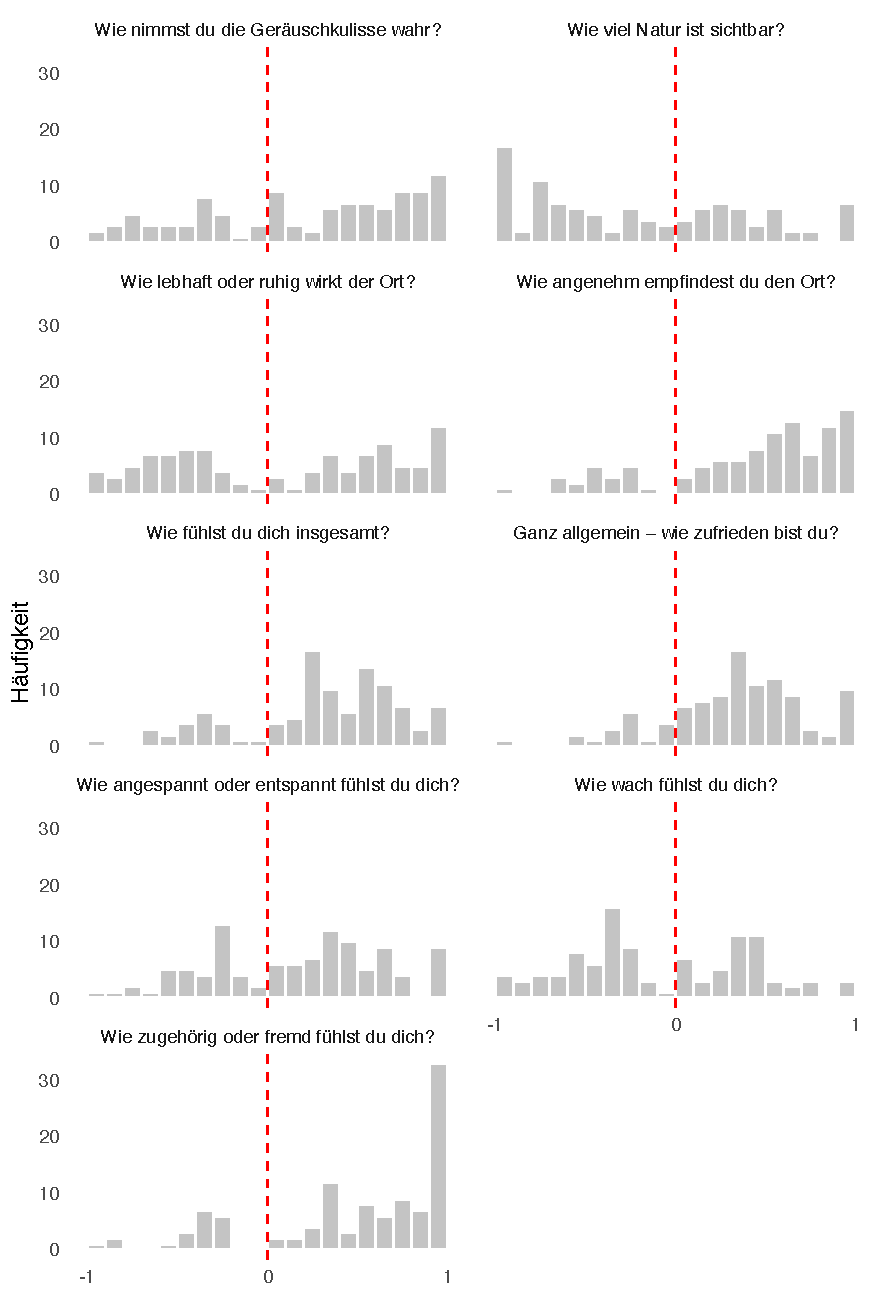
\includegraphics[width=\textwidth]{analysis/plots/slider_hists.pdf}
    \caption{Histogramme der Slider-Items}
    \label{fig:slider_hists}
\end{figure}

\begin{longtable}{p{5.5cm}p{9.5cm}}
    \caption{Antworten auf Freitextfragen}
    \label{tab:freitext}\\
    \toprule
    Frage & Antwort \\
    \midrule
    \endfirsthead

    \multicolumn{2}{c}{{\bfseries Tabelle \thetable{} -- Fortsetzung}} \\
    \toprule
    Frage & Antwort \\
    \midrule
    \endhead
    
    \midrule
    \multicolumn{2}{r}{Fortsetzung auf der nächsten Seite}\\
    \endfoot
    
    \bottomrule
    \endlastfoot

    Gibt es andere Dinge die dazu führen, dass Du dich hier weniger wohl oder unwohl fühlst? & heat \\*
     & Everyone is doing the same, so it kind of feels like being at the right place \\*
     & The contact with strangers \\*
     & Bed \\*
     & health issues \\*
     & no natural sunlight room without windows no fresh air \\*
     & a lot of people - personal space \\*
     & No \\*
     & / \\*
     & no \\*
     & Not really \\
    \midrule
    \addlinespace
    Gibt es andere Dinge die dazu führen, dass Du dich hier wohler fühlst? & place i know and is mine i have control over it \\*
     & know this place and can do what i want \\*
     & my room and cozy for the night \\*
     & pets \\*
     & spending time with family pets \\*
     & I am not by myself \\*
     & Less noise from construction works \\
    \bottomrule
\end{longtable}


\addtocontents{toc}{\protect\setcounter{tocdepth}{2}}

\end{appendices}
%TC:endignore
\end{document}